\documentclass[
  % Replace twoside with oneside if you are printing your thesis on a single side
  % of the paper, or for viewing on screen.
  oneside,
  %twoside,
  11pt, a4paper,
  footinclude=true,
  headinclude=true,
  cleardoublepage=empty
]{scrbook}

\usepackage{dissertation}
\usepackage[T1]{fontenc}
\usepackage{textcomp}
\usepackage[titles]{tocloft}
\usepackage{xcolor}

\setlength{\cftbeforechapskip}{2ex}
\setlength{\cftbeforesecskip}{0.5ex}

\renewcommand{\cftpartfont}{%
  \fontsize{12}{14}\usefont{OT1}{phv}{bc}{n}\selectfont
}
\renewcommand{\cftchapfont}{%
  \fontsize{11}{13}\usefont{OT1}{phv}{bc}{n}\selectfont
}
\renewcommand{\cftsecfont}{%
  \fontsize{10}{11}\usefont{OT1}{phv}{}{n}\selectfont
}
\renewcommand{\cftsubsecfont}{%
  \fontsize{9}{10}\usefont{OT1}{phv}{}{n}\selectfont
}
\renewcommand{\cftfigfont}{%
  \fontsize{9}{10}\usefont{OT1}{phv}{}{n}\selectfont
}
\renewcommand{\cfttabfont}{%
  \fontsize{9}{10}\usefont{OT1}{phv}{}{n}\selectfont
}

\usepackage[all]{xy}
\usepackage{circuitikz}

\titleA{Automated and Intelligent Hacking Detection System}
\author{Bruno Alves Martins Carvalho}
\supervisor{José Bacelar Almeida}
\cosupervisor{Luís Sobral Silva}
\date{\myear}

\makeglossaries
\newacronym{gps}{GPS}{Global Positioning System}
\newacronym{lte}{LTE}{Long-Term Evolution}
\newacronym{ids}{IDS}{Intrusion Detection System}
\newacronym{can}{CAN}{Controller Area Network}
\newacronym{iot}{IoT}{Internet of Things}
\newacronym{adas}{ADAS}{Advanced Driver-Assistance Systems}
\newacronym{ecu}{ECU}{Electronic Control Unit}
\newacronym{sdk}{SDK}{Software Developer Kit}
\newacronym{lin}{LIN}{Local Interconnect Network}
\newacronym{most}{MOST}{Media Oriented Systems Transport}
\newacronym{tpms}{TPMS}{Tire Pressure Monitoring System}
\newacronym{vanet}{VANET}{Vehicular Ad Hoc Network}
\newacronym{obd}{OBD}{On-Board Diagnostics}
\newacronym{iso}{ISO}{International Organization for Standardization}
\newacronym{csma}{CSMA}{Carrier-Sense Multiple-Access}
\newacronym{cdamp}{CP+AMP}{Collision Detection and Arbitration on Message Priority}
\newacronym{rnn}{RNN}{Recurrent Neural Network}
\newacronym{ann}{ANN}{Artificial Neural Network}
\newacronym{lstm}{LSTM}{Long Short-Term Memory}
\newacronym{gru}{GRU}{Gated Recurrent Unit}
\newacronym{dnn}{DNN}{Deep Neural Network}
\newacronym{dbn}{DBN}{Deep Belief Network}
\newacronym{cnn}{CNN}{Convolutional Neural Network}
\newacronym{rbm}{RBM}{Restricted Boltzmann Machines}
\newacronym{ocsvm}{OCSVM}{One Class Support Vector Machine}
\newacronym{dos}{DoS}{Denial of Service}
\newacronym{hmm}{HMM}{Hidden Markov Model}
\newacronym{htm}{HTM}{Hierarchical Temporal Model}
\newacronym{gmm}{GMM}{Gaussian Mixture Model}
\newacronym{svm}{SVM}{Support Vector Machine}
\newacronym{csv}{CSV}{Comma Separated Values}
\newacronym{ip}{IP}{Internet Protocol}
\newacronym{autosar}{AUTOSAR}{Automotive Open System Architecture}
\newacronym{swc}{SWC}{Software Components}
\newacronym{bsw}{BSW}{Basic Software}
\newacronym{vfb}{VFB}{Virtual Function Bus}
\newacronym{rte}{RTE}{Runtime Environment}
\newacronym{io}{IO}{Input-Output}
\newacronym{ota}{OTA}{Over-the-Air}
\newacronym{v2d}{V2D}{Vehicle-to-Device}
\newacronym{v2v}{V2V}{Vehicle-to-Vehicle}
\newacronym{v2i}{V2I}{Vehicle-to-Infrastructure}
\newacronym{v2n}{V2N}{Vehicle-to-Network}
\newacronym{v2x}{V2X}{Vehicle-to-Everything}
\newacronym{dsrc}{DSRC}{Dedicated Short Range Communication}
\newacronym{its}{ITS-5G}{Intelligent Transport Systems operating in the 5 GHz frequency range}

\begin{document}\fontfamily{phv}\fontseries{mc}\selectfont

%!TEX root = dissertation.tex

\makeatletter

% UM_ENg Logo
\def\UMEng#1#2{\begin{tikzpicture}[
	% bars styling,
	logone/.style={rectangle,fill=white,rounded corners=0.08cm,minimum width=0.16cm,inner sep=0pt},
	bigone/.style={minimum height=0.74cm},
	smaone/.style={minimum height=0.48cm},
	engone/.style={minimum height=0.86cm},
	pos1/.style={xshift=1.3cm,yshift=1.3cm},
	pos2/.style={xshift=3.9cm,yshift=1.3cm}]
	
% Uminho logo
	\fill[fill=#1] (0,0) -- (2.6,0) -- (2.6,2.6) -- (0,2.6) -- cycle;
	\foreach \i in {1,...,3}{
		\node at (\i*120+30:0.45)[logone,bigone,pos1,rotate=\i*120-60]{};
		\node at (\i*120+90:0.60)[logone,smaone,pos1,rotate=\i*120]{};
	}

% EngUminho logo
	\fill[fill=#2] (2.6,0) -- (5.2,0) -- (5.2,2.6) -- (2.6,2.6) -- cycle;
	\foreach \i in {1,...,5}
		\node at (\i*72-90:0.74)[engone,logone,pos2,rotate=\i*72-90]{};
\end{tikzpicture}}

\def\yyy#1{\fontfamily{phv}\fontseries{mc}\selectfont {\ifnum\hide=1\relax\else#1\fi}}
\def\xxx#1{\fontfamily{phv}\fontseries{mc}\selectfont #1}
\def\zzz#1{\fontfamily{phv}\fontseries{mc}\fontseries{b}\selectfont #1}
\def\kkk#1{\fontfamily{phv}\fontseries{mc}\fontseries{b}\selectfont {\ifnum\hide=1\relax\else#1\fi}}

\long\def\coverEtc{
%Logo
~\vskip-4.1cm\rule{4cm}{0pt}\begin{tabular}{l}
\UMEng\umc{eng}
\\\zzz{Universidade do Minho}\rule{0pt}{1cm}
\\\xxx{}{Escola de Engenharia}
\\\xxx{Departamento de  Informática}
\\\rule{0pt}{4cm}
\\\xxx{{\Large\@author}}
\\\rule{0pt}{1em}
\\\zzz{\Large\@titleA}
\\\zzz{\Large\@titleB}
\\\zzz{\Large\@titleC}
\\\rule{0pt}{5cm}
\\\yyy{\large Master dissertation}
\\\yyy{\large Integrated Master’s in Informatics Engineering}
\\\rule{0pt}{6mm}
\\\yyy{\large Dissertation supervised by}
\\\kkk{\@supervisor}\rule{0pt}{4mm}
\\\kkk{\@cosupervisor}
\\\rule{0pt}{4.2cm}
\\\xxx{{\small\@date}}
\end{tabular}
}


\begin{frontcover}
\gdef\umc{um}\gdef\hide{1}
\thispagestyle{empty} \pagecolor{white} \textcolor{black} \coverEtc
\end{frontcover}

\begin{titlepage}
\gdef\umc{um}
\gdef\hide{0}
\thispagestyle{empty} \pagecolor{white}\textcolor{grey} \coverEtc
\end{titlepage}

\makeatother


\cleardoublepage

\pagenumbering{alph}
\setcounter{page}{0}

\chapter*{Copyright and Terms of Use for Third Party Work}

This dissertation reports on academic work that can be used by third parties as long as the internationally accepted standards and good practices are respected concerning copyright and related rights.
\vskip 1em
\noindent This work can thereafter be used under the terms established in the license below.
\vskip 1em
\noindent Readers needing authorisation conditions not provided for in the indicated licensing should contact the author through the RepositóriUM of the University of Minho.

\section*{License granted to users of this work:}

\CCBY

\chapter*{Acknowledgements}

% Em primeiro lugar, agradecer ao meu orientador que semore me orientou e me motivou com os seus belos ocmentarios, nomeadamente "está muito catita" \par
% Ao luís, bla bla bla\par
% E por fim, o mais importante, agradeço à minha namorada, Dra. Sílvia Azevedo Costa cédula profissional 74166, pelo seu apoio constante desde o primeiro dia da construçºao desta tese, quando ainda nem sabia o tema e o estava a discutir numa esplanada na sé. Linda, és o meu suporte, inspiraste-me a escrever sobre carros, apesar de seres um helicoptero. 
\cleardoublepage

\chapter*{Statement of Integrity}

I hereby declare having conducted this academic work with integrity.
\vskip 1em\noindent
I confirm that I have not used plagiarism or any form of undue use of information or falsification of results along the process leading to its elaboration. 
\vskip 1em\noindent
I further declare that I have fully acknowledged the Code of Ethical Conduct of the University of Minho.

\chapter{Abstract}

% The first vehicles had very few, if any, electronic components. This has been changing gradually, primarily driven by the consumer's expectations of more features and comfort in their vehicles, and by ever-stricter government regulations on efficiency and emissions. Today, practically every function of the vehicle is controlled electronically via \glspl{ecu} connected by various bus technologies such as the \gls{can}, \gls{lin}, and the emerging Automotive Ethernet. Such technology raises the risk of attacks, especially now that vehicles are connected to the exterior via Bluetooth, Wi-Fi, and cellular, and hold sensitive information about the driver. Traditional networks, such as IP, typically have an \gls{ids} analysing traffic and signalling when an attack occurs. The system here proposed is an adaptation of the traditional IDS into the CAN bus, since CAN is the primary bus connecting most nodes, and its protocol does not have any security functionality such as encryption or message authentication. The proposed IDS uses a \gls{ocsvm} trained with features extracted from live, attack-free traffic, to reliably detect a variety of attacks, both known and unknown, without needing to understand the syntax of the packet's payload, which is largely proprietary. This allows the system to be installed in any vehicle in a plug-and-play fashion while maintaining a large degree of accuracy with very few false positives.

The \gls{can} in the backbone of automotive networking, connecting many \glspl{ecu} that control virtually every vehicle function from fuel injection to parking sensors. It possesses, however, no security functionality such as message encryption or authentication by default. Attackers can easily inject or modify packets in the network, causing vehicle malfunction and endangering the driver and passengers. There is an increasing number of \glspl{ecu} in modern vehicles, primarily driven by the consumer's expectation of more features and comfort in their vehicles as well as ever-stricter government regulations on efficiency and emissions. Combined with vehicle connectivity to the exterior via Bluetooth, Wi-Fi, or cellular, this raises the risk of attacks. Traditional networks, such as \gls{ip}, typically have an \gls{ids} analysing traffic and signalling when an attack occurs. The system here proposed is an adaptation of the traditional \gls{ids} into the \gls{can} bus using a \gls{ocsvm} trained with live, attack-free traffic. The system is capable of reliably detecting a variety of attacks, both known and unknown, without needing to understand payload syntax, which is largely proprietary and vehicle/model dependent. This allows it to be installed in any vehicle in a plug-and-play fashion while maintaining a large degree of accuracy with very few false positives.

\paragraph{Keywords} intrusion detection system, machine learning, controller area network, connected vehicles
\cleardoublepage
\chapter*{Resumo}

% Os primeiros veículos possuíam muito poucos componentes eletrónicos. Isto tem vindo a mudar gradualmente, impulsionado principalmente pelas expectativas dos consumidores quanto ao aumento de conforto nos seus veículos, e pelos cada vez mais exigentes regulamentos de eficiência e emissões. Hoje, praticamente todas as funções do veículo são controladas eletrónicamente via Unidades de Controlo Eletrónico (UCEs) ligadas através várias tecnologias de transmissão tais como a Controller Area Network (CAN), a Local Interconnect Network (LIN), e a emergente Automotive Ethernet. Tais tecnologias aumentam o risco de ataques, especialmente agora que os veículos estão ligados ao exterior via Bluetooth, Wi-Fi, e rede móvel, e possuem informação sensível acerca do condutor. Redes tradicionais, como o IP, possuem tipicamente um Sistema de Deteção de Intrusão (SDI) que analiza o tráfego e sinaliza quando ocorre um ataque. O sistema aqui proposto é uma adaptação do SDI tradicional à CAN, uma vez que a CAN é a principal tecnologia de comunicação que liga a maior parte dos nodos, e não possui qualquer funcionalidade direcionada à segurança, como cifragem ou autenticação das mensagens. O SDI proposto utiliza uma One Class Support Vector Machine (OCSVM) treinada com dados extraídos de tráfego real, livre de ataques, para detetar com viabilidade uma variedade de ataques, tanto conhecidos como desconhecidos, sem a necessidade de entender a sintaxe do campo de dados das mensagens, que é maioritariamente proprietária. Isto permite ao sistema ser instalado em qualquer veículo num modo \textit{plug-and-play} enquanto mantém um elevado nível de desempenho com muito poucos falsos positivos.

A \gls{can} é a principal tecnologia de comunicação interna automóvel, ligando muitas \glspl{ecu} que controlam virtualmente todas as funções do veículo desde injeção de combustível até aos sensores de estacionamento. No entanto, não possui por defeito funcionalidades de segurança como cifragem ou autenticação. É possível aos atacantes facilmente injetarem ou modificarem pacotes na rede causando estragos e colocando em perigo tanto o condutor como os passageiros. Existe um número cada vez maior de \glspl{ecu} nos veículos modernos, impulsionado principalmente pelas expectativas do consumidores quanto ao aumento do conforto nos seus veículos, e pelos cada vez mais exigentes regulamentos de eficiência e emissões. Isto, associada à conexão ao exterior através de tecnologias como o Bluetooth, Wi-Fi, ou redes móveis, aumenta o risco de ataques. Redes tradicionais, como a rede \gls{ip}, tipicamente possuem um \glspl{ids} que analiza o tráfego e assinala a presença de um ataque. O sistema aqui proposto é uma adaptação do \gls{ids} tradicional à rede \gls{can} utilizando uma \gls{ocsvm} treinada com tráfego real e livre de ataques. O sistema é capaz de detetar com fiabilidade uma variedade de ataques, tanto conhecidos como desconhecidos, sem a necessidade de entender a sintaxe do campo de dados das mensagens, que é maioritariamente proprietária. Isto permite ao sistema ser instalado em qualquer veículo num modo \textit{plug-and-play} enquanto mantém um elevado nível de desempenho com muito poucos falsos positivos.

\paragraph{Palavras-chave} sistema de deteção de intrusão, aprendizagem máquina, controller area network, veículos conectados
\cleardoublepage
\pagenumbering{roman}
\setcounter{page}{3}

\cleardoublepage
\phantomsection
\addcontentsline{toc}{chapter}{Contents}
\tableofcontents

\cleardoublepage
\listoffigures

\cleardoublepage
\listoftables

\cleardoublepage
\pagenumbering{arabic}
\setcounter{page}{8}

\part{Introductory material}
\chapter{Introduction}
\label{c:intro}

Computation and networking were first introduced in the 1970s out of the manufacturer's necessity to meet new and stringent emissions regulations \citep{pelkmans2003trends}. Then, the concept of connected cars appeared in Formula 1 in 1980, with the vehicle being able to transmit data to the pitlane \citep{bmwConnectedCar}. In 1996, General Motors introduced its OnStar roadside assistance program, where the vehicle could register an accident and automatically call the nearest emergency centre \citep{sspiConnectedCar}. The use of \gls{gps} by civillians was allowed in May of 2000, which not only improved navigation but also allowed stolen vehicles to be tracked \citep{bmwConnectedCar}. Remote diagnostics were introduced in 2001 and, since then, we saw the inclusion of vehicle health reports and 4G \gls{lte} networking. Manufacturers are currently working on adding 5G connectivity to their vehicles. This networking ability makes the modern vehicle a part of the \gls{iot}. Not only are vehicles more connected than ever, but they also have much more computing power. Many modern vehicles offer at least some driving assistance functionality and make decisions to avoid accidents.\par

This increase in functionality means that a modern car contains about 100 million lines of software code, and is expected to have around 300 million lines of code by 2030. For comparison, a passenger plane has around 15 million \citep{yahooCarSecurity}. This leaves a lot of room for vulnerabilities to appear, and many attacks have been successfully demonstrated. These include not only locking and unlocking the vehicle, and information theft, but also disruption of safety-critical components such as sensors and brakes \citep{Kim2021}. Manufacturers have, however, failed to keep up with the cybersecurity needs of the vehicles they produce. The two main reasons for this issue are that first, automakers specialised in the manufacturing of vehicles and not in software engineering, and second, there is an increased cost to making secure software \citep{forbesSecurityCost}.\par

Here, a prototype of an \gls{ids} for \gls{can}, which is currently the dominant networking protocol in the automotive industry, is presented. \glspl{ids} are common in traditional IP networks, but their implementation in \gls{can} is still being explored. Most proposed IDS methodologies are very resource heavy, with complex deep learning models often being implemented \citep{ahmad2021network}. This results in lower energy efficiency, which is of major importance to both the manufacturers and the customer. The system here presented performs blind traffic analysis, meaning that it does not need to understand packet syntax. Since this is non-standardised and highly proprietary information, it allows the system to be installed in a variety of vehicles. It is also design to work in an embedded environment, constrained by the limited computing resources that are present in a vehicle as well as its efficiency goals.\par

This dissertation is organised as follows. In Chapter \ref{c:background}, an overview of relevant concepts is first conducted. This includes modern vehicle software architectures, followed by automotive security standards, common attacks, and proposed solutions. Automotive in-vehicle networks are then detailed, before an in-depth look at the \acrlong{can} is taken. Relevant machine-learning concepts are then introduced.\par
A look into the state-of-the-art of \glspl{ids} is performed in Chapter \ref{c:sota}. It details modern detection approaches, along with evasion techniques, and goes over recent literature on the adaptation of the \gls{ids} concept into the \acrlong{can}. Automotive-specific challenges are also explored, followed by an approach to incident response.\par
% Chapter \ref{c:contribution} begins the dissertation's core content. It describes how this application is relevant and how it contributes to progress in the field of automotive cybersecurity.\par
Datasets used to develop and test the application are listed in Chapter \ref{c:datasets}. These vary from publicly available datasets to ones gathered from a real vehicle cluster for the purposes of this dissertation.\par
The proposed application is detailed in Chapter \ref{c:application}. The general architecture is first explained, followed by the training process and the features extracted from network traffic. The application's execution in an embedded environment, along with its options, concludes this chapter.\par
Test results are presented in Chapter \ref{c:results}, with Chapter \ref{c:limitations} presenting the application's limitations and detailing future work.\par
Chapter \ref{c:conclusion} concludes the dissertation.
\chapter{Background}
\label{c:background}

\section{Modern vehicles}

In recent years, vehicles have become ever smarter, providing functionality that goes beyond simple transportation of passengers and goods. They can guide us through \gls{gps}, make calls, receive over-the-air updates, inform other vehicles of their position, and even drive themselves. Having this computational capacity, being identifiable, able to transfer data over a network and connected to each other makes modern vehicles a part of the \acrlong{iot} \citep{Lombardi2021}.\par

\subsection{Applications}

A significant part of automotive innovation has been driven by software applications. These take advantage not only of the data generated by internal sensors to perform complex tasks but allow for better multimedia functionality and communication with external entities. In \cite{Le2018}, the authors classify automotive applications based on the following criteria: functional domain, influence on safety, driver involvement, connectivity, and time constraint.\par

The functional domain encompasses powertrain, chassis, body, passive safety, telematics and \gls{adas}. Influence on safety describes how a misbehaving application potencially affects safety, and can go from \emph{not safety-related}, to \emph{safety-related}, and finally \emph{safety-critical}. The degree of the driver's involvement determines how much attention the driver must devote to the alerts that an application generates. The sort of connectivity needed by an application is defined by connectivity. In certain applications, only the vehicle's ECUs are used. V2D, V2V, V2I, or V2N connections could be necessary for some other applications. Time constraint is degree to which an application must adhere to a given response time. If sometimes missing deadlines has no significant consequences, the program is considered \emph{soft real-time}. It is \emph{hard real-time} if an application must constantly stick to a predetermined response time and missing a deadline might result in major issues. Otherwise, a program is \emph{non real-time} if there are no restrictions on response time.\par

The main application domains for a modern vehicle are shown in Figure \ref{fig:Car_Domains}. These are powertrain, chassis, body control, infotainment, and telematics and communications. Powertrain and chassis control vehicle dynamics, with applications like engine and transmission control being a part of the powertrain domain, and driving assistance and safety being a part of the chassis domain. The body control domain is responsible for non-dynamic vehicle applications, such as climate control, dashboard, lights, windows, mirrors, seats, etc. Radio, CD/DVD player, \gls{gps}, among others, are part of the infotainment domain. Diagnostic applications, for example, are located in the telematics and communications domain. Emerging \gls{adas} applications are, however, breaking this separation as their complexity requires data and computation from multiple different domains in order to safely assist the driver in controlling the vehicle. These include adaptive cruise control, lane-assist, and automatic emergency braking.

\begin{figure}
    \centering
    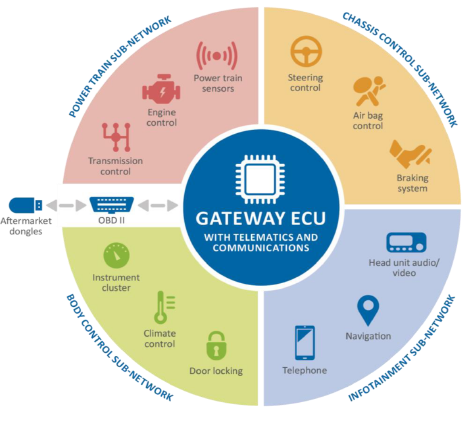
\includegraphics[width = .7\textwidth]{img/parts/introduction/Vehicle Architecture.png}
    \caption{Main domains of a modern car \citep{ENISA}}
    \label{fig:Car_Domains}
\end{figure}

Such an increase in computational complexity allows for the introduction of vulnerabilities in the software and, with applications extending multiple domains and interacting with other applications, there is an increased concern about their security. Until recently, applications were developed by the manufacturers to run directly on the embedded hardware. The usual approach was to add a new \gls{ecu} for every new function to be implemented. However, this method has made the vehicle’s internal network too complex for safe and efficient handling. Therefore, a platform-based approach has become of interest to both manufacturers and developers as it provides developers with an abstraction of the underlying hardware as well as making it possible to write reusable applications to run on the same standardised platform, but different hardware. This simplifies both the application development as well as its deployment. Besides, the authors in \cite{Holle} suggest that an approach like that of the mobile platforms could be taken. In this case, an open \gls{sdk} is provided to third-party developers to create and distribute their applications similarly to mobile app stores.\par

This increase in application diversity and functionality means that the vehicle handles much more sensitive information, especially when considering its connectivity to devices as personal as one’s smartphone. This includes information like common routes and schedules, call history, or even conversations recorded with the internal microphones (otherwise used for phone conversations on virtual assistances). As such, modern vehicles are becoming a major target for attackers who seek to obtain information on the user, not only because they contain sensitive information, but also because of the lack of security elements present in the vehicle design and architecture. This is because manufacturers have always designed their vehicles with safety, but no security in mind \citep{Siegel2018}.

\subsection{Architecture}

In all of these domains, \glspl{ecu} are responsible for controlling their components, such as precise fuel combustion in the powertrain domain or air conditioning in the body control domain. These controllers are often based on the ARM platform, with an automotive-grade product line generally being used due to unique constraints in the automotive environment. Together, they can be tought as the vehicle's distributed computer.\par

In 2003, the \gls{autosar} was established as a "worldwide development partnership of vehicle manufacturers, suppliers, service providers and companies from the automotive electronics, semiconductor and software industry" with the objective of creating an open and standardised software architecture for \gls{ecu} \citep{autosar}. The use of such a manufacturer independent standard allows for a reduction in development effort and improved software quality, as software modules can be used in vehicles of different manufacturers and component suppliers, thereby reducing complexity and expense. \gls{autosar} maintains five standards: the \gls{autosar} Classic Platform, the \gls{autosar} Adaptive Platform, the Foundation, \gls{autosar} Acceptance Tests, and \gls{autosar} Application Interfaces.\par

The \gls{autosar} Classic architecture is shown in Figure \ref{fig:autosar_arch}. It is composed of three software layers which run on a microcontroller: the Application Layer, \gls{rte}, and \gls{bsw}. The \gls{rte} handles communication between the application layer, which is mostly hardware independent, and the \gls{bsw}. The \gls{bsw} is then divided intro three layers, along with complex drivers: services, \gls{ecu} abstraction, and microcontroller abstraction. Services are further divided into functional groups representing the infrastructure for system, memory and communication services.

\begin{figure}
    \centering
    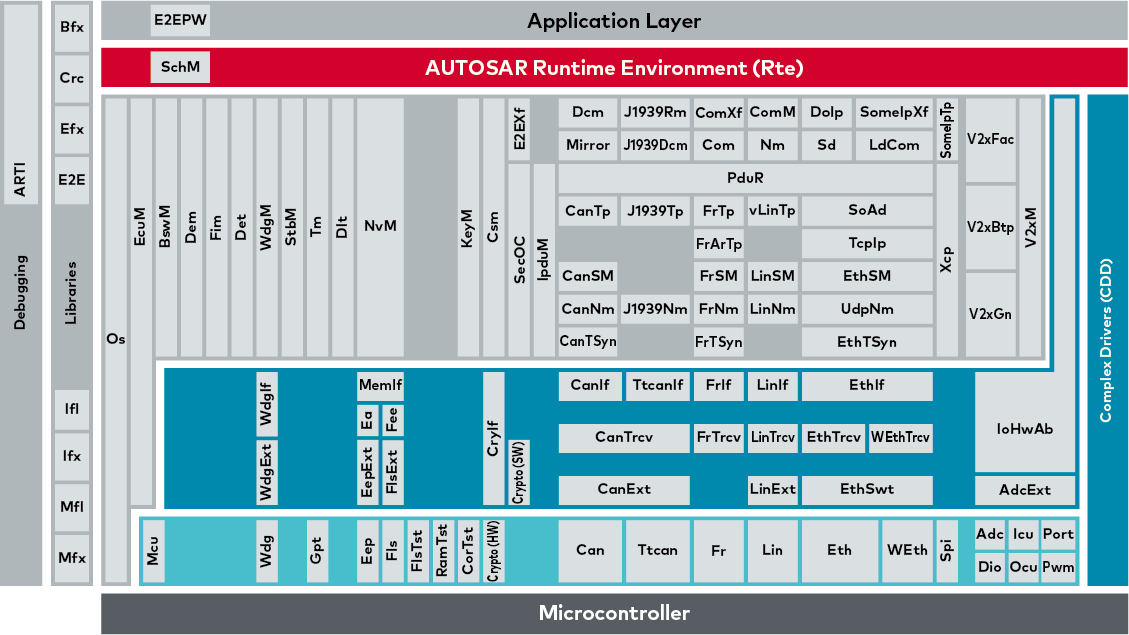
\includegraphics[width = \linewidth]{img/parts/introduction/AUTOSAR.png}
    \caption{The \gls{autosar} architecture \citep{autosar_arch}}
    \label{fig:autosar_arch}
\end{figure}

The \gls{vfb} allows for communication between different applications (\glspl{swc}) and the use of \gls{bsw} services, both within the individual \gls{ecu} and between \glspl{ecu}. Because the development of \glspl{swc} is based on the \gls{vfb}, \glspl{swc} are independent of the underlying hardware, making them easier to reuse and integrate into different projects on different platforms as well as to flexibly relocate existing \glspl{swc} to \glspl{ecu} during development.\par

New use cases, such as autonomous driving, communication with traffic infrastructure, multimedia applications, and smartphone integration, led to the creation of the \gls{autosar} Adaptive Platform. This standard aims to provide support for the deployment of customer applications and an environment for applications that require a high amount of computing power (\textit{e.g.} computer vision). It implements the \gls{autosar} Runtime for Adaptive Applications, with a POSIX-based operating system at its core running \citep{autosar_adaptive_os} on virtualized hardware. In contrast to the \gls{autosar} Classic Platform, the \gls{autosar} Runtime Environment for the Adaptive Platform dynamically links services and clients during runtime. This allows applications to be developed, tested and distributed or updated independently of one another.

\begin{figure}
    \centering
    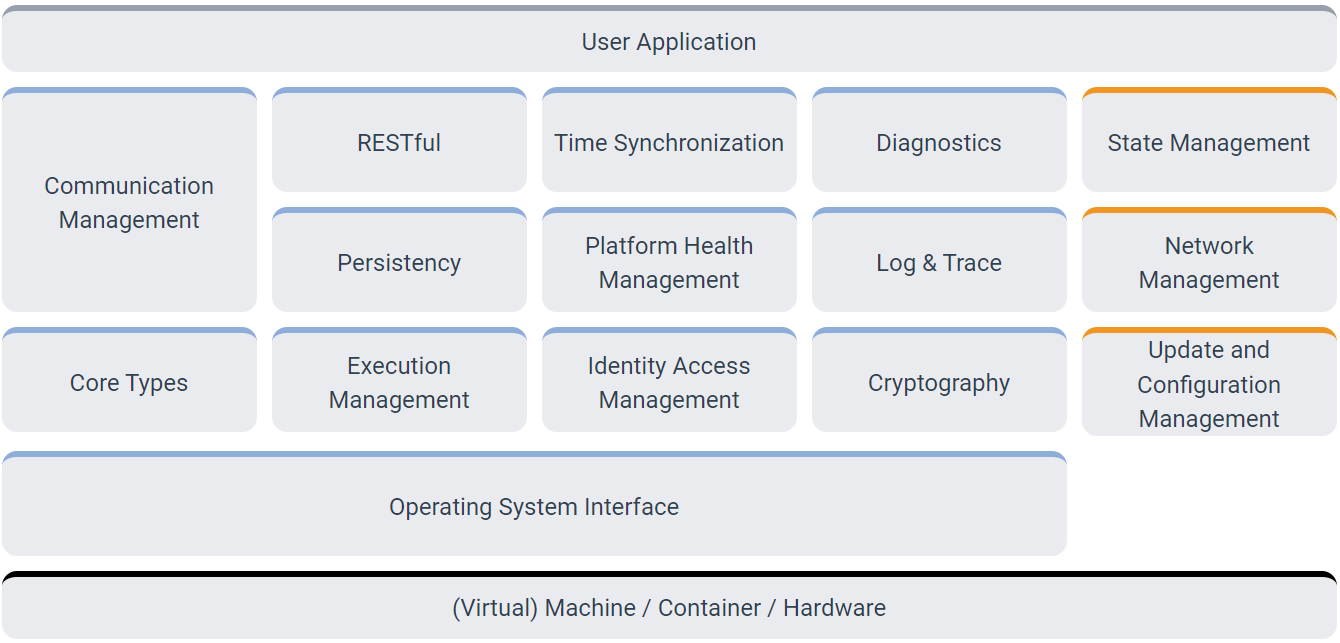
\includegraphics[width = \linewidth]{img/parts/introduction/AUTOSAR Adaptive Platform.png}
    \caption{The AUTOSAR Adaptive Platform architecture \citep{autosar_adaptive_arch}}
    \label{fig:autosar_adaptive_arch}
\end{figure}

The Foundation standard enforces interoperability between the \gls{autosar} platforms by the means of common requirements and technical specifications shared between them, \textit{e.g} bus protocols and common aspects of the methodology.\par

Acceptance Tests for Classic Platform are system tests that validate \gls{autosar} stack behaviour at the bus and application level. \gls{autosar} provides tests that cover \gls{rte} requirements, \gls{bsw} services, and bus protocols and behaviour. It also allows for the addition of tests by the user to certify specific features not covered in the standard set.\par

The Application Interfaces standard covers syntax and semantics for the body and confort, powertrain engine, powertrain transmission, chassis control, ocupant and pedestrian safety, and human-machine interface, multimedia and telematics domains. The deployment of standardised application interfaces assures software reusability independently of specific hardware and/or \glspl{ecu}, which is one of the main requirements of \gls{autosar}.

\subsection{External communication}

Modern vehicles have a variety of ways of communicating with the exterior. Use cases include communicating with wireless keys, sensors, other vehicles, smartphones, and road infrastructure. It is common to classify these types of vehicle communication according to the following categories:

\begin{itemize}
    \item \acrfull{v2d}: Communication with a device inside the vehicle.
    \item \acrfull{v2v}: Communication with another vehicle.
    \item \acrfull{v2i}: Communication with road infrastructure.
    \item \acrfull{v2n}: Communication with IT or cellular infrastructure.
\end{itemize}

The term \acrlong{v2x} is used to refer to general vehicle communication.\par

Either the head unit or the telematics control unit conducts communication. A head unit often includes a screen, telephone, navigation, and interfaces for connecting to other consumer electronics. An exclusive \gls{ecu} that offers wireless communication is a telematics control unit. Based on access range, interfaces may be divided into three major groups: physical access, short-range wireless access, and long-range wireless access \cite{Le2018}.

\subsubsection{Physical access}

The interface that needs physical access the most is the one for diagnosis. Regulations for \gls{obd} (such as OBD-II in the United States, EOBD in the European Union, or JOBD in Japan) demand the monitoring and detection of deterioration, dysfunction, and electrical failures in emission systems. This port allows for the requesting of stored data about faults, real-time data from sensors and \glspl{ecu}, reading and setting fault codes, and controlling actuators. It also alows access to vehicle data in non-diagnostic mode.\par
Other physical access interfaces include CD/DVD players and USB ports.

\subsubsection{Short-range wireless access}

One use for these interfaces is to link sensors and actuators to the in-vehicle network, such as tire pressure monitoring systems and keyless entry (TPMS).\par
Bluetooth and WiFi are dominant in the telematics domain. Bluetooth is commonly used for hands-free phone calls and music playback, while WiFi can be used for \gls{ota} updates and Internet tethering between vehicles.\par
Other protocols exist for ad-hoc \gls{v2v} and \gls{v2i} communication, such as \gls{its} in Europe, and \gls{dsrc} in the United States. They are both based on the IEEE 802.11p standard at the physical layer. \gls{its} has four channels for separate purposes: safety applications, non-safety applications, wireless local area networks, and a channel reserved for future applications. Although \gls{dsrc} primarily focuses on safety applications, it is also utilized in toll collection, navigational aid, and garage door openers.

\subsubsection{Long-range wireless access}

Communication at distances over 1 km is considered long-range and can be classified into wither broadcast or adressable channels. Signals can be sent to multiple vehicles, whose address is unknown, using a broadcast channel. Services like \gls{gps} or digital radio are examples of this type of communication. On the other hand, addressable channels are used to send messages to specific devices. These channels are provided by cellular networks and can be used for Internet access or voice transmission.

\section{Security Standards}

Functional safety is already an integral part of road vehicle engineering, with the functional safety norm \cite{ISO26262} being well established. The industry's pursuit to design and build safer connected vehicles is leading to the development of several secure software development standards for the automotive sector. One such standard is the \cite{ISO21434} Road Vehicles - Cybersecurity Engineering. It's predecessor, \cite{SAEJ3061}, already established some high-level guiding principles such as defining a complete lifecycle process framework, and it also recommends an initial assessment of potential threats and risks that may be considered relevant.\par

An overview of the ISO/SAE 21434:2021 can be found on Figure \ref{fig:iso21434toc}. Clause 4 offers some general considerations and contextualises the approach to vehicle cybersecurity taken in the standard. Clause 5 concerns the organisational structure, and describes the organisation's security objectives and how to achieve those objectives as well as responsibility and authority assignment. Clause 6 discusses cybersecurity management at the project level, detailing, among others, the proposed approach for tailoring and incorporating off-the-shelf components. Clause 7 describes cybersecurity responsibility distribution between customer and supplier. Clause 8 details the continuous development activities, such as risk assessment and vulnerability management, until the end of cybersecurity support. Clause 9 concerns the concept phase, which involves considerations of vehicle functionality as well as the cybersecurity goals for each item. Clauses 10 and 11 discuss the product development phase, including the specification of cybersecurity requirements and architectural design, as well as integration and verification activities and the validation of cybersecurity goals and claims. Clauses 12 to 14 describe the components of the post-development phase, such as production (manufacturing and assembly of an item or component), operations and maintenance (including cybersecurity incident response), and end of support and decommissioning. Finally, Clause 15 discusses threat analysis and cybersecurity risk assessment.

\begin{figure}
    \centering
    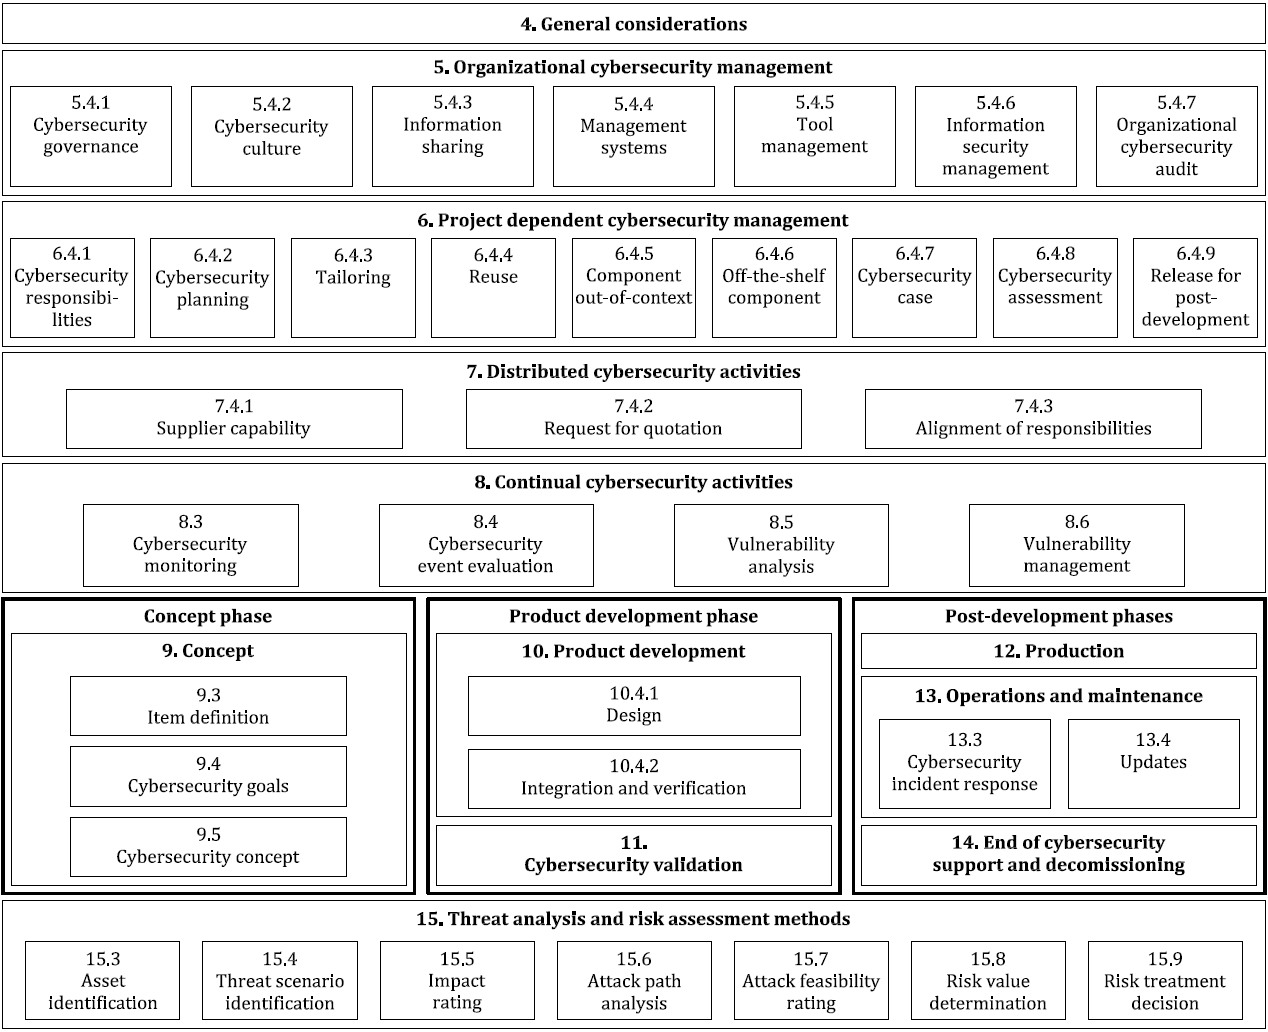
\includegraphics[width = \textwidth]{img/parts/introduction/ISO 21434 ToC.png}
    \caption{Content overview of the \cite{ISO21434}}
    \label{fig:iso21434toc}
\end{figure}

\section{Automotive cybersecurity}

\subsection{Objectives}

The CIA triad is a common way of refering to the fundamental elements of information security. The three key terms are:

\begin{itemize}
    \item \textbf{Confientiality}, meaning that information is accessible only to those with proper authorisation. This first became important when manufacturers were conserned with \gls{ecu} firmware, which contains intelectual property. More recently, it became a more general concern due to the personal information that the vehicle stores, such as adress book and location history.
    \item \textbf{Integrity}, requiring that information is modified only in an authorised manner. Integrity includes authentication, which calls for the ability of the recipient of a communication to confirm the message's provenance. Information that causes a vehicle to react, \textit{e.g.} automated braking, must be authentic both in terms of its source and its content.
    \item \textbf{Availability}, requiring that services are fully available to authorised users.
\end{itemize}

As security concerns grow due to the connecivity of complex applications these aim to fullfil these common security requirements. Moreover, privacy is also a concern, as \gls{v2v} and \gls{v2i} applications could share messages containing personally identifiable information, such as location and the identity of the vehicle's occupants.

\subsection{Common attack patterns}

The authors of \cite{Kim2021} surveyed previously published research on attacks against autonomous vehicles, although some attacks are also effective against non-autonomous vehicles. They classify attack research into three categories: attacks on the automotive control system, attacks on the autonomous driving system components, more specifically through mobile apps, and attacks on Vehicle-to-Everything (V2X) communication technologies.

\subsubsection{Automotive control systems}

One type of automotive control system attack targets the vehicle’s \glspl{ecu}. Taking advantage of network vulnerabilities, research shows that it is possible to load firmware into \glspl{ecu} that control components such as the door-lock and telematics, primarily through fuzzing \citep{Koscher2010}. The vulnerabilities described by \cite{rouf2010security} showed that it is possible for an attacker to remotely display a false tire pressure warning or disable the \gls{tpms} \gls{ecu}, as well as vehicle tracking from 10-40 metres. More recently, it was shown that \glspl{ecu} present in Tesla vehicles could be controlled remotely by sending arbitrary \gls{can} packets, which led Tesla to introduce code-signing protection in an Over-The-Air (OTA) update \citep{Nie2017}. \cite{miller2015remote} showed that, even remotely, and attacker can reprogram \glspl{ecu}, control display and sound systems, the instrument cluster, body components, interfere with the engine operation, lock and disable brakes, prevent the car from turning on or off, etc. They showed that, even from telematics \glspl{ecu}, this type of attack has the same effects as directly injecting messages into \gls{can} buses.\par

In-vehicle network attacks aim to disrupt communication between vehicle components. In \citep{Palanca2017}, the authors showed that the \gls{can} bus is vulnerable to selective \gls{dos} attacks, which cannot be detected at the frame level. Sniffing and replay attacks have also been demonstrated, as per \cite{hoppe2009applying}. \cite{nilsson2009first} also explored possible attacks on the FlexRay protocol. They showed that, because there is no encryption, it is possible to read all data sent to the bus, as well as insert unauthenticated messages. A successful attack causes serious disruption of the vehicle control system and may harm drivers and passengers.\par

Passive key-less entry and start systems used in modern cars are a major attack target. It has been shown that some systems are vulnerable to relay attacks by duplicating the existing signal \citep{francillon2011relay}. Through the analysis of cryptographic vulnerabilities, \cite{verdult2012gone} demonstrated how private keys could be recovered from the Hitag2 transponder in order to bypass the key's cryptographic authentication in as little as 6 minutes. \cite{garcia2016lock} also showed how to recover cryptographic keys and clone a VW group remote via eavesdropping on a single signal, as well as another Hitag2 attack able to clone the remote in just a few minutes.\par

\subsubsection{External communication technologies}

A comprehensive survey of attacks on \glspl{vanet} \cite{Hasrouny2017} showed that these are vulnerable to the same attacks as a regular network, such as \gls{dos}, man in the middle, message suppression, or spoofing.\par

The integration of Bluetooth has become standard, and it brings with it a new set of vulnerabilities. In \cite{Cheah2017}, it was shown that manufacturers still include the ability to use legacy pairing, which led the authors to identify vulnerabilities. Other research has shown the execution of attacks using Bluetooth as a vulnerable component, as shown in \cite{Cai2019} with BMW cars.

\subsubsection{Mobile apps}

The increase in connectivity between the driver’s vehicle and his smartphone led to an expansion in the vehicle’s attack surface. A malicious smartphone app could be used to gain unauthorised access to a vehicle without needing to be in its proximity (i.e., using long-range wireless networks). The authors of \cite{Woo2015} exploited \gls{can} vulnerabilities in the process of demonstrating this scenario. Vulnerabilities in the MirrorLink protocol have also allowed attackers to send \gls{can} packets through a smartphone, opening the possibility for a variety of exploits. The attack method present in \cite{mazloom2016security} took advantage of a heap overflow. A vulnerability in Blue Link, a vehicle control application from Hyundai Motors, allowed the recovery of the driver's username, password, and PIN. An attacker could also exploit this vulnerability to remotely unlock the vehicle \citep{toddbluelink}. With the smartphone being relatively vulnerable to attacks, and with manufacturers providing more functionality to it's connection to the vehicle, it is expected that these type of applications become a major target \citep{Kim2021}.

\subsection{Proposed solutions}

The development of protection mechanisms faces multiple constraints resulting from the limited computing resources available to each \gls{ecu} as well as the time-sensitive nature of their operations. There is also a need to assert retro-compatibility with currently used embedded technologies, and, when considering external entities, interoperability between their security mechanisms. Two distinct vehicles, for example, should not be prevented from communicating because their protocols are incompatible \citep{Studnia2013}.\par

There is an effort by European projects such as Secure Vehicular Communication (SeVeCom) \citep{Kargl2008}, Preparing Secure Vehicle-to-X Communication Systems (PRESERVE) \citep{PRESERVE}, or E-safety Vehicle Intrusion Protected Applications (EVITA) \citep{EVITA}, to design secure vehicle communication architectures.\par

For \glspl{vanet}, the usage of public-key infrastructure has also been proposed, to assert the authenticity of the messages, as well as the use of pseudo-anonymity to preserve privacy. For preventing \gls{dos} attacks, some routing protocols have also been studied \citep{Hasrouny2017}.\par

Regarding internal protection, there have been several attempts to leverage cryptography in securing the \gls{ecu} and the \gls{can} bus. An authentication protocol, such as the one proposed in \citep{Herrewege2011} or \citep{Groza2018}, would prevent most injection attacks. Another approach, taken by the EVITA project, consists in the implementation of a dedicated hardware module for cryptographic operations \citep{Wolf2011}.\par

\gls{ids} has traditionally been used in network security, more specifically in desktop IT. \citep{hoppe2009applying} is one of the first to mention its usage in automotive IT as a “promising supplemental measure”. They also discuss a way to optimally communicate a warning to the driver.

\section{In-vehicle networks}

For a long time, the only electronic component in a vehicle was the radio. However, pushes for more environmentally friendly vehicles, as well as increased comfort, led to the addition of many more electronic modules. These can be a part of several subsystems, such as the powertrain, chassis, body, and infotainment system, each with its own set of requirements. These requirements may be an assurance of message delivery and minimum delivery times for safety-critical applications, or high bandwidth for infotainment purposes. Longevity must also be considered. In \cite{AvgCarAge}, it was shown that the average car age in the European Union is 11.5 years. For comparison, the average smartphone lifespan for consumers in the United States has been documented to be around 2.75 years \citep{AvgPhoneAge}. Network boot-time is relevant as well, as automotive boot-time should remain under 100ms, while some smartphones take over 1 minute to boot \citep{AutomotiveNetworks}. Power consumption must not be forgotten, as it impacts the vehicle's range. The manufacturer's desire to reduce the vehicle's complexity, weight, and cost, led to the use of a heterogeneous set of networks with different characteristics.\par

\cite{AutomotiveNetworks} lists some roles that a network might serve. These are safe/time-critical data, control data, backbone, infotainment, multi-gig data, and low cost/speed data. Below is an introduction to some of the dominant automotive network protocols, and a general overview of these networks can be seen in Table \ref{fig:auto_networks}.

\begin{table}
    \centering
    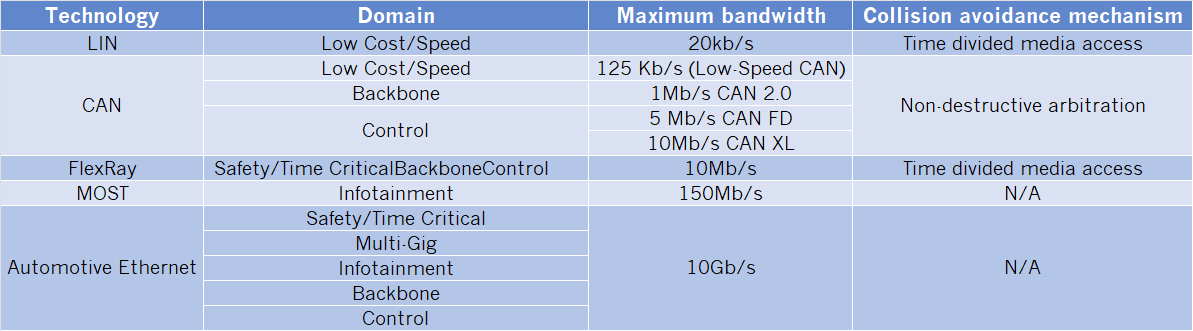
\includegraphics[width = \textwidth]{img/parts/introduction/Network Table.png}
    \caption{Characteristics of dominant automotive networks}
    \label{fig:auto_networks}
\end{table}

\subsection{Controller Area Network}
\label{subsec:can}

The development of the \gls{can} standard was started in 1983 by Uwe Kiencke. It was first introduced in February of 1986 at the Society of Automotive Engineers Congress by Robert Bosch GmbH \citep{can}. Following the publication of \gls{can} 2.0 by Bosch in 1991, the \gls{iso} released the \gls{can} standard ISO 11898. The Mercedes W140, first available in 1991, was the first vehicle with a \gls{can}-based in-vehicle network \citep{CAN_Merc}.\par

\gls{can} messages are sent in broadcast mode, which means that all \glspl{ecu} in a network receive all transmissions. Devices that receive a message acknowledge their reception. Each \gls{ecu} listens for messages from a subset of IDs, and each message ID must be sent by no more than one \gls{ecu} \citep{kulandaivel2019canvas}. It was designed with the objective of building a low-cost, and reliable network, and is therefore used mainly used for powertrain, chassis and body electronics. Its limited bandwidth of 1Mb/s does not allow for its use in other domains, such as the infotainment system \citep{Huang2019}.\par

A deeper look into \gls{can} is conducted in Section \ref{s:can}.

\subsection{Local Interconnect Network}

\gls{lin} is a supplement to the \gls{can} bus, offering lower performance and reliability, but also a much lower cost. It is a product of the \gls{lin} Consortium, founded by BMW, Volkswagen Group, Audi, Volvo Cars Mercedes-Benz, Volcano Automotive Group, and Motorola, and provides cost-efficient communication in applications where the bandwidth and versatility of \gls{can} are not required. This typically includes mechatronic nodes like the vehicle’s windows, wipers, side mirrors, or seat controllers \citep{LIN}.\par

The first version of the specification was released in 1999, with updates soon following. \gls{lin} 2.0 was released in 2003 and the protocol was standardised in ISO 17987:2016.\par

Unlike \gls{can}, a typical \gls{lin} cluster consists of a single commander node and up to 16 responders connected by a single copper wire, with communication speeds up to 20kbit/s \citep{Takahashi2017}. It is usually deployed as a \gls{can} sub-network, with only the \gls{lin} master node being connected to the \gls{can}-bus. All communications are initiated by the commander node, with one responder replying to a given message identifier (the commander node can also act as a responder, replying to its own messages). There is, therefore, no need to implement collision detection \citep{LIN_CSS}.\par

This protocol also implements a sleep and wake-up mechanism, allowing it to potentially save power. Responders can enter sleep via a command issued by the commander node or are forced into that state after more than 4 seconds of \gls{lin} inactivity. The wake-up command can be issued by any node \citep{LIN}.
We can see in Figure \ref{fig:auto_nodes} that the number of \gls{lin} nodes has recently surpassed the number of \gls{can} nodes.

\begin{figure}
    \centering
    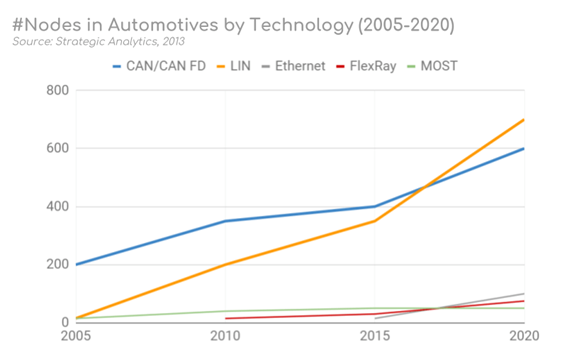
\includegraphics[width = \linewidth]{img/parts/introduction/LIN Nodes.png}
    \caption{Number of nodes in automotive by technology \citep{LIN_CSS}}
    \label{fig:auto_nodes}
\end{figure}

There have been recent efforts to study the security aspects of \gls{lin}, such as the one detailed in \citep{Takahashi2017}, and it is noted that due to its link with \gls{can}, the latter’s vulnerabilities are also a cause for concern for the former. \citep{Ernst2018} showed that a compromised \gls{lin} node can destroy as well as create "erroneous, but valid packets". The authors also suggested that the effect of an intrusion can be minimised by the use of appropriate firewalls. However, since \gls{lin} is usually used for non-safety-critical purposes, compromising the bus would most likely not be life-threatening.

\subsection{FlexRay}

The continuous search for improved safety, performance, and comfort of vehicles means that the speed and reliability of data communicated between \glspl{ecu} must increase. FlexRay was developed by the FlexRay Consortium, founded in 2000 by Daimler Chrysler and BMW along with Motorola and Phillips, and disbanded in 2009. The Consortium had the goal of creating a bus protocol capable of delivering achieving high data rate, deterministic and fault-tolerant communications \citep{FlexRayFreescale} as a way of overcoming \gls{can}'s limitations in these aspects. Features that require a higher throughput for safety/time-critical data like active cruise control, anti-lock braking system, or break-by-wire, thus use FlexRay as the preferred communication protocol, as it satisfies the reliability requirements for these safety-critical systems.\par

The FlexRay bus consists of a single twisted-pair copper cable, with \glspl{ecu} connected using multi-drop technology. Its clock synchronisation is deterministic and uses time divided media access as a collision avoidance mechanism, in contrast to the arbitration mechanism used by \gls{can}. This makes it suitable for safety/time-critical applications. It is also used for backbone and control data, similarly to \gls{can}. However, it provides much higher bandwidth: 10Mb/s, compared to \gls{can}'s maximum of 1Mb/s, and is more expensive \citep{Huang2019}.\par

The protocol is defined in \gls{iso} 17458-1 to 17458-5.

\subsection{Media Oriented Systems Transport}

As the name suggests, \gls{most} is primarily used for high-speed multimedia. It can use either a single twisted pair of copper cables, or plastic optical fibre (which has the advantage of being completely immune to electromagnetic disturbance), and supports 25, 50, and 150 Mb/s data transfer speeds \citep{MOSTMicrochip}. The \gls{most} network is capable of managing up to 64 devices, usually configured in a ring topology. Star or double ring configurations are also possible \citep{MOSTVector}, with the latter being relevant for safety-critical applications \citep{Huang2019}.\par

The \gls{most} specification, described in ISO 21806, defines the physical and data link layers, as well as all the seven layers of the \gls{iso}/OSI model.

\subsection{Automotive Ethernet}

Automotive Ethernet is an adaptation of standard Ethernet that fulfils the requirements of the automotive environment, such as the use of a single twisted-pair wiring, which provides lower cost and better electromagnetic compatibility.\par

The motivation behind this adaptation is primarily the amount of full-duplex bandwidth it provides. In 2020, IEEE published the IEEE 802.3ch-2020 standard, detailing the specification for automotive Ethernet with data transfer speeds of up to 10Gb/s (10GBASE-T1). This allows fields like \gls{adas} to grow and develop without much concern for bandwidth restrictions. Another important factor is that Ethernet is already an established technology outside of the automotive industry. This means that there is a large knowledge base to support it, especially when compared to the other protocols discussed here. Its use of the IP stack is a point in its favour as well. It is also a scalable technology, with adding new nodes to the network being a relatively easy task \citep{Bello2011}.\par

As for the network topology, Ethernet is, by nature, a point-to-point network. This means that connecting more than two nodes requires an Ethernet switch.\par

This technology does not aim, however, to only replace other high-bandwidth networks like \gls{most}. The 10BASE-T1s version of the automotive Ethernet protocol is a direct competitor to \gls{can} and FlexRay, as it describes a multi-drop bus topology network over a single twisted pair of copper wires with speeds up to 10Mb/s and time divided media access for collision avoidance \citep{AutomotiveNetworks}. This would allow for a vehicle using only IP based technologies, simplifying the overall design of the network.

\section{Controller Area Network}
\label{s:can}

\gls{can} is currently the dominant network protocol in automotive. As laid out in \ref{subsec:can}, it is a broadcast network with no central bus master, which allows for data consistency across the entire system. The two lowest layers of the ISO/OSI model for \gls{can} are defined in the ISO 11898 \citep{Richards2002} and the implementation can be seen in Figure \ref{fig:CAN_ISO}. Protocols such as the CANopen protocol, supported by the \emph{CAN in Automation} group (CiA), establish the link between the physical and data link layers and those above \citep{Corrigan2002}.

\begin{figure}
    \centering
    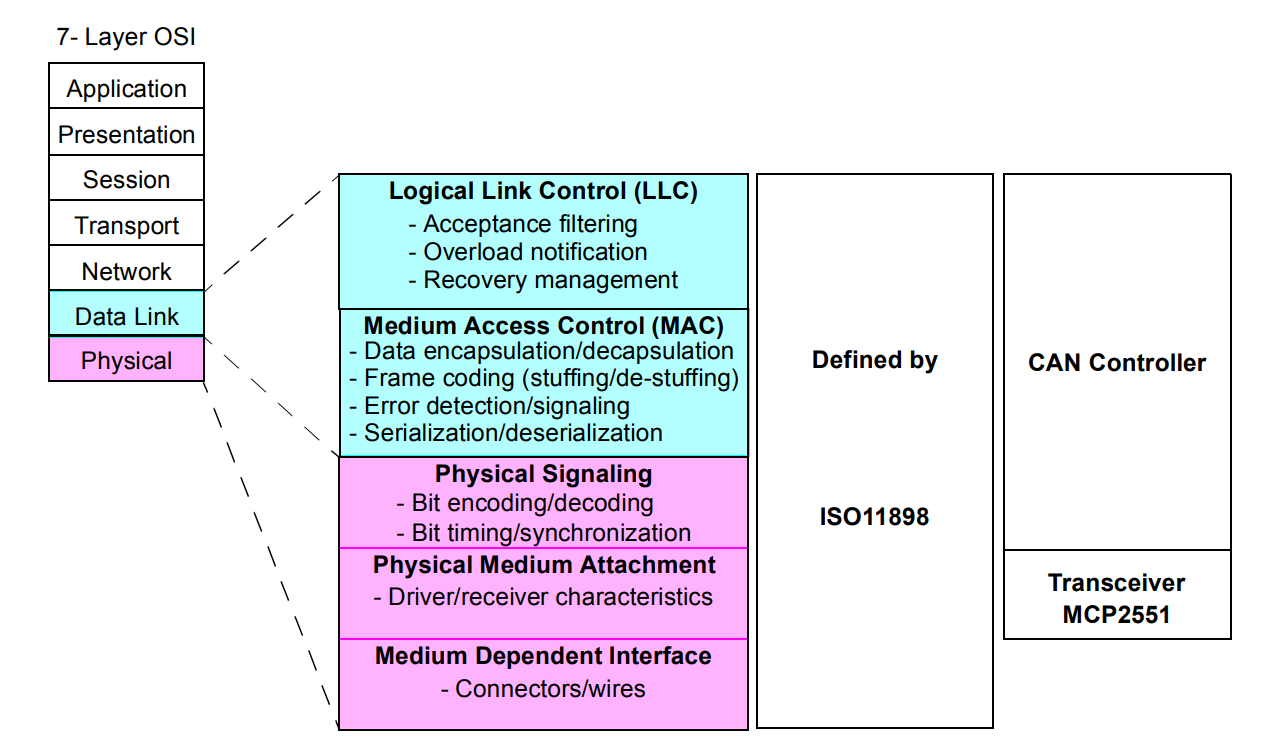
\includegraphics[width = \textwidth]{img/parts/introduction/CAN ISO.png}
    \caption{\gls{can} and the OSI model \citep{Richards2002}}
    \label{fig:CAN_ISO}
\end{figure}

The \gls{can} bus differs from a conventional bus because it inverts the logic state between the bus, driver input and receiver output. In \gls{can}, a logic high is associated with a 0 (the dominant bit), and a logic low with a 1 (the recessive bit) \citep{Corrigan2002}. An illustration of this mechanism can be seen in Figure \ref{fig:CAN_Bus_Logic}.

\begin{figure}
    \centering
    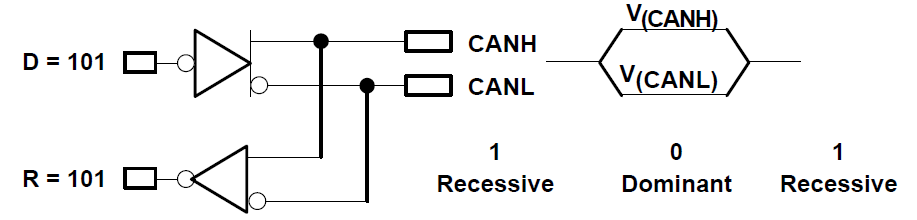
\includegraphics[width = \textwidth]{img/parts/introduction/CAN Bus Logic.png}
    \caption{The inverted logic of a \gls{can} bus \citep{Corrigan2002}}
    \label{fig:CAN_Bus_Logic}
\end{figure}

\gls{can} uses \gls{csma}, meaning that each node must wait for bus inactivity before transmitting, with \gls{cdamp}, meaning that collisions are resolved through bit-wise arbitration using the message's ID field. Messages with lower ID have a higher priority, as a smaller identifier will hold the dominant state on the bus for longer \citep{Corrigan2002}. The bus can, therefore, be thought of as acting as an AND gate, as explained by \cite{Cook2008}.\par

There are four message types in \gls{can}: the data frame, the remote frame, the error frame, and the overload frame. Error-free messages have the last bit of the EOF set as recessive, and a dominant bit in this field causes the message to be re-transmitted.\par

The data frame is the most common message type and is composed of seven fields: SOF, arbitration, control, data, CRC, ACK, and EOF. The SOF field consists of a single dominant bit, and the arbitration decides which of the nodes attempting to transmit is allowed to do so. The RTR field distinguished between data (dominant bit) and remote (recessive bit) frames. The control field indicates the amount of data being sent in the data field. The remote frame is used to request a data frame from another node. If a node broadcasts a remote frame containing a particular identifier, the node responsible for this identifier immediately generates a data frame as a response. The error frame is used to notify errors in frame transmission, and the overload frame signals that the controller has not finished processing the current message, and delays the start of the next message \citep{lee2017otids}.
\gls{can} is available in three generations: Classical \gls{can}, \gls{can} FD, and \gls{can} XL. These are described below.

\subsection{Classical CAN}

There are three versions of what can be called "classical" \gls{can}: low-speed \gls{can}, \gls{can} 2.0A, and \gls{can} 2.0B. As the name suggests, low-speed \gls{can} has limited bandwidth, at 125Kb/s. However, it is fault-tolerant, as it can operate even when one of the two wires fails. This version of the protocol is standardised in ISO 11898-3. \gls{can} 2.0 versions A and B allow for speeds up to 1Mb/s, with the main difference between the two versions being that the former uses an 11-bit identifier (standard), and the latter a 29-bit identifier (extended). The bit fields for standard (low-speed \gls{can} and \gls{can} 2.0A) and extended (\gls{can} 2.0B) versions can be seen of Figures \ref{fig:standard_can} and \ref{fig:extended_can}, respectively. The meaning of the bit fields are:

\begin{itemize}
    \item \textbf{SOF (Start Of Frame)}: Single dominant bit that marks the start of a message.
    \item \textbf{Identifier}: Establishes the priority of a message (lower ID means higher priority).
    \item \textbf{RTR (Remote Transmission Request)}: When this bit is dominant, information is required from the node specified in the identifier.
    \item \textbf{SRR (Substitute Remote Request)}: Replaces the RTR bit as a placeholder in the extended format.
    \item \textbf{IDE (Identifier Extension)}: When this bit is dominant, a standard \gls{can} identifier is being transmitted.
    \item \textbf{r0}: Reserved bit.
    \item \textbf{r1}: Reserved bit.
    \item \textbf{DLC (Data Length Code)}: 4-bit field that contains the number of bytes of data being transmitted.
    \item \textbf{Data}: Up to 64 bits may be transmitted.
    \item \textbf{CRC (Cyclic Redundancy Check)}: 16-bit field containing the checksum of the transmitted data for error detection.
    \item \textbf{ACK (Acknowledge)}: Every accurate message received has this recessive bit overwritten by a dominant bit.
    \item \textbf{EOF (End-Of-Frame)}: 7-bit field that signals the end of a \gls{can} frame, while also disabling bit-stuffing.
    \item \textbf{IFS (Inter-Frame Space)}: 7-bit field that allows the controller enough time to move the received frame into the message buffer.
\end{itemize}

\begin{figure}
    \centering
    \begin{subfigure}{\textwidth}
        \centering
        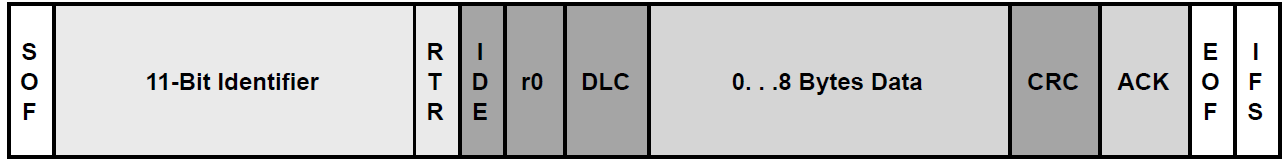
\includegraphics[width=\textwidth]{img/parts/introduction/Standard CAN.png}
        \caption{Standard \gls{can}: 11-bit identifier}
        \label{fig:standard_can}
    \end{subfigure}
    \begin{subfigure}{\textwidth}
        \centering
        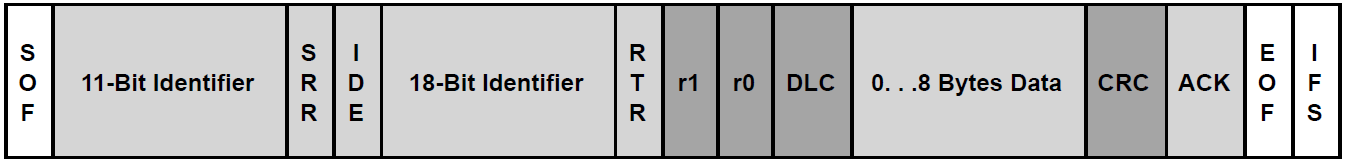
\includegraphics[width=\textwidth]{img/parts/introduction/Extended CAN.png}
        \caption{Extended \gls{can}: 29-bit identifier}
        \label{fig:extended_can}
    \end{subfigure}
    \caption{Classical \gls{can} frame structure \citep{Corrigan2002}}
\end{figure}

\subsection{CAN FD}

Increasing demand for more bandwidth led to the development of \gls{can} FD (standing for Flexible Data-Rate), which was started in 2011 by Robert Bosch GmbH. The fact that this design is based on \gls{can} 2.0 provides several advantages. Costs are similar, and it has a small impact on current software and applications. The physical layer and topologies can also be maintained \citep{Woo2016}. It is primarily used in high-performance vehicle \glspl{ecu} and is established as an international standard in ISO 11898-2:2015.\par

The main difference between \gls{can} 2.0 and \gls{can} FD is the flexible data rate that \gls{can} FD offers. This means that it allows for the data frame to be transmitted at different speeds, depending on the characteristics of the network. Development was faced with two main challenges: avoiding increased message delays caused by placing more bytes of data in a single frame, and maintaining \gls{can}'s practical wiring \citep{CANFD}. The solution to this was the introduction of a new frame structure, which can be seen in Figure \ref{fig:CANFD_Frame}.

\begin{figure}
    \centering
    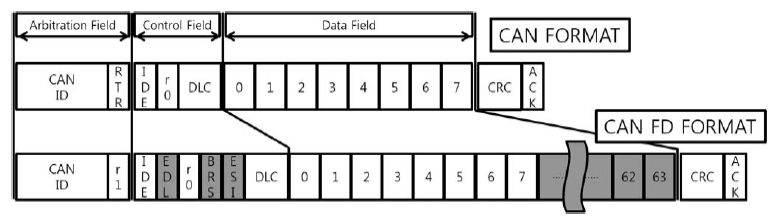
\includegraphics[width = \textwidth]{img/parts/introduction/CAN FD.png}
    \caption{Comparison of \gls{can} and \gls{can} FD data frames \citep{Woo2016}}
    \label{fig:CANFD_Frame}
\end{figure}

In the arbitration field, we can see that the RTR bit is not present in the \gls{can} FD frame. This is because there are no remote frames in \gls{can} FD.\par

Three new bits were added to the control field: extended data length (EDL), bit rate switch (BRS), and error state indicator (ESI). The EDL bit is used to distinguish between the classical \gls{can} (bit is dominant) and the \gls{can} FD (bit is recessive) frame formats. If the BRS bit is dominant, it signals that the data frame is sent at the arbitration rate (i.e. up to 1Mb/s). Otherwise, the remaining part of the data frame is sent at a higher speed (around 5Mb/s). The ESI bit is used for identifying an error in the \gls{can} FD node.\par

The CRC has also been updated from 15 bits in classical \gls{can} to 17 or 21 bits in \gls{can} FD. Lastly, the payload portion of the frame stops at the ACK bit, which means that this is the end of the potentially higher bit rate. An illustration of this can be seen in Figure \ref{fig:CANFD_BitRates}.

\begin{figure}
    \centering
    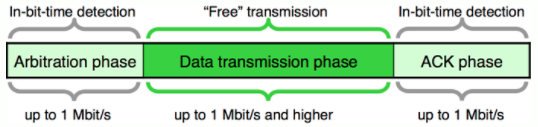
\includegraphics[width = \textwidth]{img/parts/introduction/CAN FD Bit Rates.png}
    \caption{Illustration of the \gls{can} FD flexible data-rate mechanism \citep{CANFD}}
    \label{fig:CANFD_BitRates}
\end{figure}

There exists also an extended version of \gls{can} FD, shown in Figure \ref{fig:CANFD_Extended}. It functions much like the classical extended \gls{can}, allowing for more IDs to be used.

\begin{figure}
    \centering
    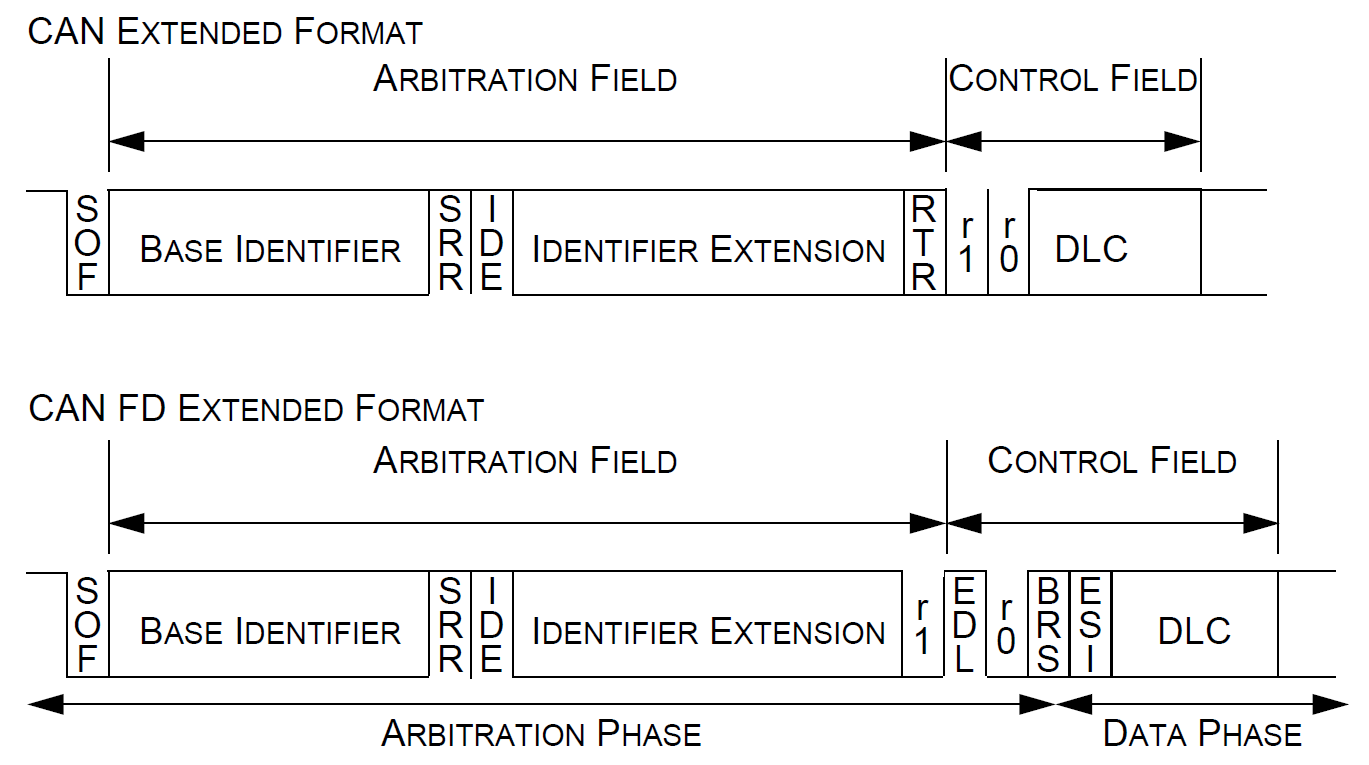
\includegraphics[width = \textwidth]{img/parts/introduction/CAN FD Extended.png}
    \caption{Comparison of extended \gls{can} and \gls{can} FD data frames \citep{Bosch2012}}
    \label{fig:CANFD_Extended}
\end{figure}

A major challenge in securing \gls{can} has been the limited speed and payload size, as it makes it difficult to implement typical cryptographic schemes, such as authentication, to defend against attacks. \gls{can} FD brings some relief in this matter, and new techniques have been proposed, like the ones in \citep{Woo2016} and \citep{Agrawal2019}.

\subsection{CAN XL}

Fueled by much of the same objectives as \gls{can} FD, as well as the rise in popularity of automotive Ethernet, \gls{can} XL presents itself as the third generation of \gls{can}, capable of providing speeds above 12Mb/s in the frame's data phase (the arbitration phase of the frame maintains its top bit-rate of 1Mb/s). This puts both 10BASE-T1s Ethernet and \gls{can} XL at the same level in terms of bit rate.\par

In contrast to 10BASE-T1s Ethernet, \gls{can} XL offers a wider range of topologies to choose from, meaning that not all \gls{can} XL networking topologies can be exactly replaced with Ethernet, as the latter has a stricter bus topology. An example of this can be seen in Figure \ref{fig:EthernetCANXL_Topologies}. The increase in data field length for \gls{can} XL also allows for transparent Ethernet frame tunnelling, enabling the use of IP communication \citep{BoschCANXL}. Another advantage this protocol has over automotive Ethernet is the fact that it is much easier to upgrade existing \gls{can} networks to \gls{can} XL than it is to transition to Ethernet and the IP stack, which is more complex and requires more expensive controllers \citep{VectorCANXL}. Seen as though \gls{can} XL can be mixed with \gls{can} FD, it also allows manufacturers to optimise cost by using the cheaper technology where higher bandwidth is not required \citep{BoschCANXL}.

\begin{figure}
    \centering
    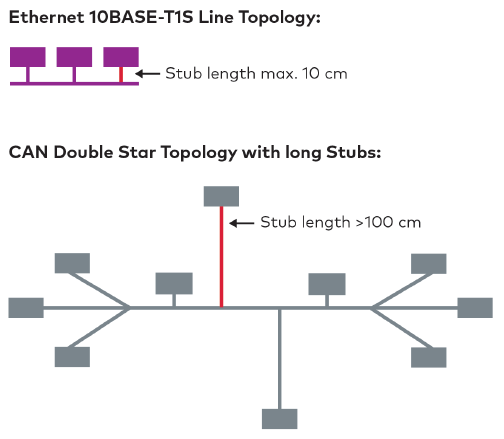
\includegraphics[width = \textwidth]{img/parts/introduction/Ethernet and CAN XL Topologies.png}
    \caption{Comparison between 10BASE-T1s and \gls{can} XL topology requirements \citep{VectorCANXL}}
    \label{fig:EthernetCANXL_Topologies}
\end{figure}

The \gls{can} XL frame structure can be seen in Figure \ref{fig:CANXL_Frame}.

\begin{figure}
    \centering
    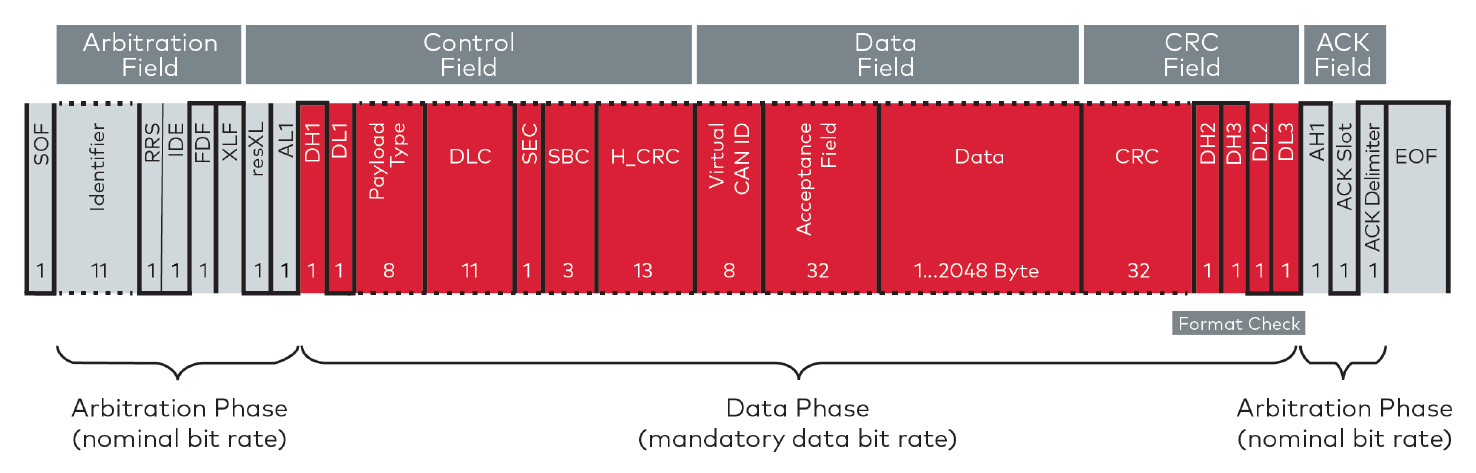
\includegraphics[width = \textwidth]{img/parts/introduction/CAN XL.png}
    \caption{Current status of development of the \gls{can} XL frame \citep{VectorCANXL}}
    \label{fig:CANXL_Frame}
\end{figure}

In Classical \gls{can} and \gls{can} FD, the \gls{can}-ID field (11 bit or 29 bit) is used for both arbitration and addressing purposes. In \gls{can} XL these functions are separated. The \gls{can} XL protocol separates the priority functions (11-bit Priority ID) and the addressing (32-bit AF). The 11-bit Priority Field provides the uniquely assigned priority of the \gls{can} XL DF. The 32-bit AF (Acceptance Field) is included in the 64-bit hardware acceptance filter of the \gls{can} XL controller. It may contain node address or content-indicating information.\par

The \gls{can} XL DF includes two CRC (cyclic redundancy check) fields: the 13-bit PCRC (Preamble CRC) in Control Field and the 32-bit FCRC (Frame CRC) in CRC Field. The CRCs are cascaded, which means the FCRC protects the whole frame, including the PCRC. Both CRCs can detect any five randomly distributed bit-errors, which corresponds to a Hamming distance of 6 \citep{CiACANXL}. New in the control field are also the possibilities to indicate the payload type, much like the EtherType field in Ethernet, and a virtual \gls{can} ID, allowing the separation of the \gls{can} network into virtual networks and comparable to the VLAN ID in Ethernet \citep{BoschCANXL}.\par

\gls{can} XL, therefore, presents itself as an incremental upgrade step for existing \gls{can} and \gls{can} FD networks, while also closing the gap in transmission speed between \gls{can} and automotive Ethernet. It aims to be a reliable alternative to 10BASE-T1s, with a simpler protocol stack and cheaper controllers. The fact that it allows for Ethernet frame tunnelling may also open the doors to joint single-based communication in the lower levels of the network (\gls{can}) and signal-based communication at the higher end (10BASE-T1s) \citep{VectorCANXL}.

\subsection{Vulnerabilities}

The reason \gls{can} is so dominant in the automotive networking space is because of its simplicity. This has, however, become an exploitable property with the exterior connectivity that did not exist when the protocol was developed.\par

Because messages are broadcast to the entire network, an attacker with access to one part of the network, like an ODB port, can eavesdrop on all traffic as well as send messages to all nodes. When eavesdropping, messages can be easily interpreted because there is no encryption in the protocol. There is also no authentication methods that allow nodes to know the source of the received frame, meaning that nodes cannot assert if a received frame was sent by a legitimate node or a bad actor. The ID-based arbitration scheme also facilitates Denial of Service attacks, as flooding the system with high-priority messages would cause all others to back off \citep{scalas2019automotive}.

\section{Machine learning}

As stated in \ref{sec:ids_detection_approaches}, the use of machine learning in an \gls{ids} allows it to adapt and detect previously unseen attacks. Such an approach has two phases: training and testing. First, attributes and classes from the training data must be identified. These must be reduced to a subset of those most relevant for classification, discarding unnecessary ones (\textit{i.e.}, dimensionality reduction). Then, the resulting dataset is used to train the model, with the trained model being used to classify unknown data. The training data can be unlabelled, which creates an unsupervised learning problem, partially labelled, for semi-supervised learning, or fully labelled, making the learning phase supervised \citep{Buczak2016}.\par

In \citep{Shearer2000}, the CRoss Industry Standard Process for Data Mining (CRISP-DM) was presented as a six-phase model describing the data science life cycle in a industry, tool, and application neutral way. A representation of this can be see in Figure \ref{fig:CRISP-DM}.

\begin{figure}
    \centering
    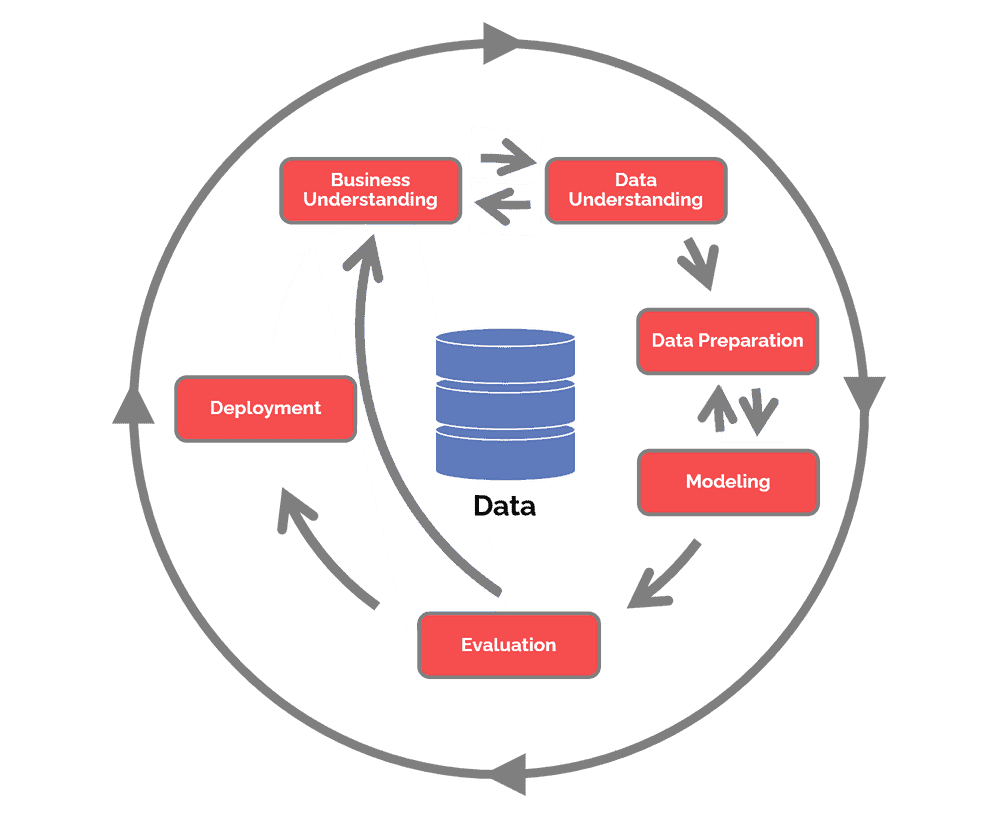
\includegraphics[width = .7\textwidth]{img/parts/introduction/CRISP-DM.png}
    \caption{CRISP-DM diagram \citep{DSPA}}
    \label{fig:CRISP-DM}
\end{figure}

The model's six phases are:

\begin{itemize}
    \item \textbf{Business understanding}, where the project's requirements are defined.
    \item \textbf{Data understanding}, where data is collected and examined.
    \item \textbf{Data preparation}, where the collected data is processed to produce the final dataset.
    \item \textbf{Modeling}, where machine learning methods are applied to produce the model.
    \item \textbf{Evaluation}, to verify whether the produced model is able to verify the requirements established in the first phase.
    \item \textbf{Deployment}, with the model being implemented.
\end{itemize}

In most applications, machine learning models are trained and then used for a long time without any modifications. In the security space, however, new threats emerge frequently. This means that models must be updated often in order to learn to detect new and emerging attack, as well as in cases where the network traffic suffers modifications in its usual pattern. Training times are, therefore, important. The model's ability to learn incrementally is also valuable, as training from scratch every time new data appears would be very time consuming.\par

Network traffic also generates a huge amount of unlabelled data, and labelling it is a laborious task. Quickly acquiring novel attack data can also be difficult, but is necessary to update the model as soon as possible \citep{Buczak2016}.\par

Deep learning is a subset of machine learning where the neural networks have more than one hidden layer. While machine learning algorithms make use of labelled and structured data to make predictions, deep learning algorithms automate feature extraction and can ingest and process unstructured data \citep{ibmDeepLearning}.

\subsection{Performance metrics}

There are several metrics used to classify a model's performance. To access if the model will generalise to an independent dataset, cross validation techniques are commonly used. Cross validation consists of a re-sampling method that iterates several times over a given dataset, sampling distinct training and test sets each time. This is particularly useful if the amount of available data is small.\par

For binary classification tasks, the confusion matrix provides several useful performance metrics by laying out true and false positives, as well as true and false negatives in a 2x2 table. Many relevant metrics can be inferred from these values, as shown in Figure \ref{fig:confusion_matrix}. The true-positive rate, also known as recall or sensitivity, provides the rate at which the model detects a truly positive case, while the false-negative rate is the proportion of positive cases missed. The false-positive rate is the probability of the model classifying a negative case as positive, and the true-negative gives the rate at which the model correctly identifies negative cases. Prevalence is the proportion of the dataset that is actually positive, while accuracy tells us how many correct predictions (both positive and negative) the model made in proportion to the total dataset. The positive predictive value metric, or precision, represents the likelihood that a positive prediction is actually positive, with the false discovery rate being its complement. The negative predictive value and false omission rate are analogous. The positive and negative likelihood ratios tell the probability that a classification is actually positive or negative is the model classifies it at such. The diagnostic odds ratio provides a way to measure the model's performance without, unlike accuracy, being affected by prevalence. The F1 score is a function of both precision and recall to give an overall indication of the classifier's performance.

\begin{figure}
    \centering
    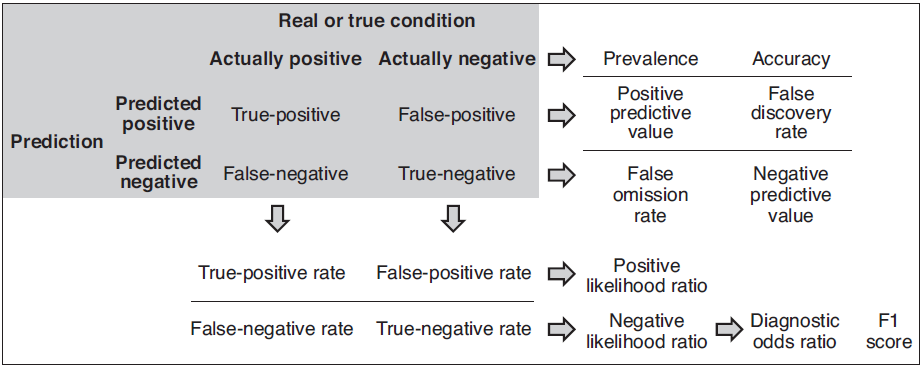
\includegraphics[width = .7\textwidth]{img/parts/introduction/Confusion Matrix.png}
    \caption{Components of a confusion matrix \citep{Handelman2019}}
    \label{fig:confusion_matrix}
\end{figure}

Another widely used metric for evaluating performance in binary classification tasks is the area under the receiver operating characteristic curve (AUROC). The curve is a graphical plot that illustrates the true-positive versus false-positive rates as the discrimination threshold is varied. A variation in the discrimination threshold usually means a gain in one metric, but a loss in the other, \textit{e.g.} a higher threshold value will decrease the classifier's recall, but increase its precision, and vice-versa. Good performing classifiers will have a large area under the plotted curve.\par

For regression problems, the mean squared error (MSE) is generally used as a way to evaluate how good the model's predictions are (\textit{i.e.}, how close they are to the true value). The MSE is calculated as the mean or average of the squared differences between predicted and expected target values in a dataset, where a lower value is preferred. The rooted mean square error (RMSE) is an extension of the MSE where the units of the metric are the same as the units of the target value (and not its square). The mean absolute error, unlike MSE and RMSE, does not punish large error values as harshly as the other two metrics, as its value increases linearly with the error size, and not quadratically. The coefficient of determination ($R^2$) indicates how much of the observed variations in the data are explained by the model, in which case a higher value is better \citep{Handelman2019, Brownlee2021}.

\subsection{Datasets}

Both the size and quality of the dataset are very important to achieve good model performance. For networking purposes, there are different types of data, with the most common being packet capture data and NetFlow.\par

Packet capture data consists of data captured by the networking interface, at the packet level. NetFlow is a router feature introduced by Cisco, giving it the ability to collect IP network traffic that goes through the interface, identifying packet flow. NetFlow version 5 defines a network flow as a unidirectional sequence of packets that share the exact same seven packet attributes: ingress interface, source IP address, destination IP address, IP protocol, source port, destination port, and IP type of service \citep{Handelman2019}. Table \ref{tab:network_datasets} shows a comparison between several public datasets.

\begin{table}
    \centering
    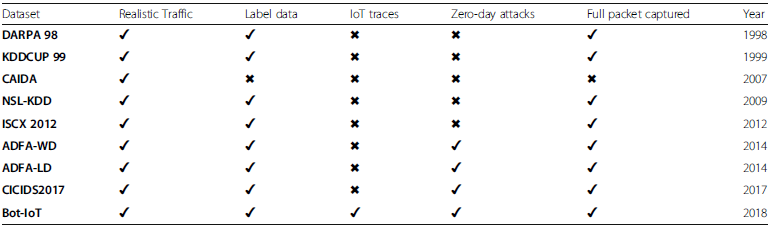
\includegraphics[width = \textwidth]{img/parts/introduction/Network Datasets.png}
    \caption{Comparison of network traffic datasets \citep{Khraisat2019}}
    \label{tab:network_datasets}
\end{table}

A majority of the effort in compiling networking datasets has been placed in the real of IP networks. In the automotive domain, there is a clear lack of such comprehensive datasets, especially when looking for labelled datasets containing attacks. Some datasets commonly used in \gls{ids} research for \gls{can} are \cite{CANDataset_OTIDS, CANDataset_Car-Hacking, CANDataset_TUE, CANDataset_IEEE}.

\subsection{Machine learning techniques}
\label{subsec:machine_learning_techniques}

\subsubsection{Supervised learning}

\paragraph{Decision trees}
A decision tree is a flowchart-like structure with three basic components: a decision node, containing the test attribute, a branch, containing a possible decision based on the attribute, and a leaf, identifying the class that the instance belongs to. The best known algorithms for constructing decision trees are the ID3 and the C4.5 algorithms \citep{Badr2014, Buczak2016}.

\paragraph{Naïve Bayes}
This technique applies Bayes' principle with assumptions that the input features are independent. It is an optimal classifier if the features are conditionally independent, although this is rarely true. One of its biggest advantages is that training can be completed in linear time \citep{Buczak2016}. The Hidden Naïve Bayes model is more sophisticated and can be applied to highly dimensional \gls{ids} tasks, with interrelated attributes and high-speed networks \citep{Khraisat2019}.

\paragraph{Evolutionary computation}
An evolutionary computation algorithm is based on the \emph{survival of the fittest} principle. Starting with a randomly generated population, a fitness value is computed for each individual from the population, revealing how good it is at solving a given problem. Fitter individuals are copied into the next generation, and the process continues. The two most widely used methods are Genetic Algorithms (GA) and Genetic Programming (GP). In GA, individuals are represented as a series of bits, to which selection and reproduction operators are applied favouring fitter solutions. In GP, individuals are represented as programs with operators (\textit{e.g.} plus, minus, and, or) and programming blocks (\textit{e.g.} if, while), and crossover and mutation operations are more complex than those in GA.

\paragraph{Artificial neural network}
The mechanisms behind an artificial neural network are similar to those of a brain. Input data is fed to a first layer of neurons, where a computation is performed and the output is fed to the next layer of neurons. The result is the output of the last layer. The model learns by looking at the error between the output and the desired outcome, and adjusting the computations, typically through backpropagation methods. For IDSs, the frequency of certain attacks in the dataset impacts how well it will be recognised, making it difficult for the model to recognise less frequent attacks \citep{Khraisat2019}.

\paragraph{Fuzzy logic}
Unlike in conventional boolean logic, where there are only true or false values, fuzzy logic allows an instance to partially belong to multiple classes at the same time, allowing for degrees of uncertainty. This makes it a good classifier for an \gls{ids}, where the border between normal and abnormal behaviour is not well defined and, therefore, reducing the rate of false alarms \citep{Khraisat2019}.

\paragraph{Support vector machines}
This classifier works by finding a hyperplane in the feature space that separates two classes so that the distance between the hyperplane and the closest data points is maximised. This is a favourable method in situations where the number of features is much greater than the number of data points \citep{Buczak2016}.

\paragraph{Hidden Markov model}
A Markov process is a stochastic model describing a sequence of states where the probability of transitioning to any particular state is dependent solely on the current state and time elapsed \citep{Maltby}. An Hidden Markov model is a statistical Markov model where the modelled system is assumed to be a Markov process with unseen data, where its states represent unobservable conditions \citep{Buczak2016}.

\paragraph{K-nearest neighbours}
The idea behind this method is to classify a point based on the $k$ nearest samples, where $k$ is the number of samples being considered. Majority voting is used to determine the classification, which can be a pitfall if the class distribution is skewed \citep{Buczak2016}.

\paragraph{Recurrent Neural Networks}
A \gls{rnn} is a feed-forward deep learning neural network in which each unit bases its decision making process on its current input and the output of the previous input. It is widely used in natural language processing and speech recognition \citep{ibmDeepLearning}. Although it can only handle limited length sequences and may suffer from short-term memory if the input length is too long, \gls{rnn} variants like \gls{lstm} and \gls{gru} have been developed to solve these issues \citep{ahmad2021network}.

\paragraph{Deep Neural Network}
A \gls{dnn} is a deep learning structure composed of an input layer, many hidden layers, and an output layer. Increasing the number of hidden layers improves the model's abstraction level, and its used to model complex nonlinear functions \cite{ahmad2021network}.

\paragraph{Deep Belief Network}
A \gls{dbn} as a deep learning model composed of stacked \gls{rbm} (a two-layer model with data flowing in both directions) in layers followed by a softmax classification layer. In a \gls{dbn}, connections exist between the layers but not between units within each layer \cite{ahmad2021network}.

\paragraph{Convolutional Neural Network}
\glspl{cnn} have three main types of layers: convolutional layer, pooling layer, and fully-connected layer. The convolutional layer is the first layer of a convolutional network. While convolutional layers can be followed by additional convolutional layers or pooling layers, the fully-connected layer is the final layer. With each layer, the network increases in its complexity, identifying greater portions of the input data. Earlier layers focus on simple features, and data progresses through the layers of the CNN, it starts to recognise larger patterns \cite{ibmCNN}.

\subsubsection{Unsupervised learning}

\paragraph{Clustering}
This is an unsupervised pattern discovery approach which groups unlabelled data based on their similarities or differences. Clustering algorithms can be exclusive, overlapping, hierarchical, and probabilistic \citep{IBM}. In exclusive clustering, a data point can exist be a part of no more than one cluster. K-means clustering is an example of an exclusive clustering algorithm, where the aim is to separate data objects into $k$ clusters, where each observation belongs to the cluster with the nearest mean. On the other hand, overlapping clustering allows a data point to be a part of multiple clusters at once (\textit{e.g.} fuzzy k-means). Hierarchical clustering seeks to create a hierarchy of clusters, and the approach can be categorised in two ways: agglomerative, which is a bottom up approach where sub-clusters are grouped together as one moves up through the hierarchy, and divisive, where the largest cluster in diameter is separated into sub-clusters \citep{Khraisat2019}. Probabilistic clustering, data points are clustered based on the likelihood that they belong to a particular distribution, with the Gaussian Mixture model being commonly used \citep{IBM}.

\paragraph{Association rules}
An association rule describes a relationship among different attributes: \emph{if (A and B) then C}, with metrics revealing how often a given relationship occurs in the data. Fuzzy association rules extend this functionality into categorical or quantitative data, instead of boolean only. These take the form of \emph{if (X is A) then (Y is B)} \citep{Buczak2016}.

\subsubsection{Statistical inference}

\paragraph{Inductive learning}
This method attempts to find patterns and regularities in the observations, and then makes general conclusions or theories about the data in the form of rules.
% RIPPER

% \subsubsection{Ensemble}

\subsection{Support Vector Machines}

As stated in \ref{subsec:machine_learning_techniques}, \glspl{svm} are a supervised machine learning model for non-probabilistic binary classification (although methods such as Platt scaling allow for it's use in a probabilistic classification setting \citep{platt1999}) through the construction of one or several hyperplanes that best separate data into distinct categories. This classifier works by mapping the input space into a higher-dimensional feature space, where separation between classes becomes easier, and finding a hyperplane that separates two classes so that the distance between the hyperplane and the closest data points is maximised \citep{Buczak2016}. New data is then classified based on their positioning relative to those hyperplanes. An example of this can be seen in Figure \ref{fig:svm_hyperplane}.

\begin{figure}
    \centering
    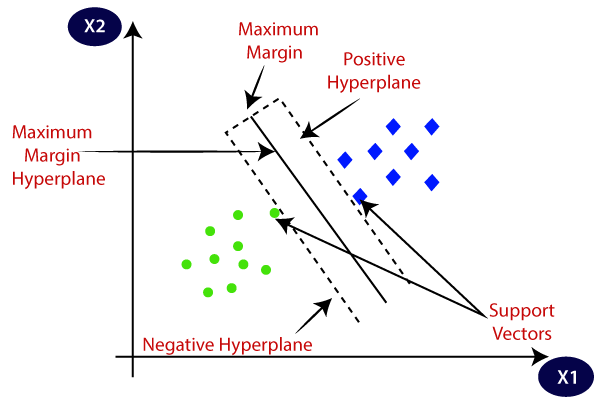
\includegraphics[width = .8\linewidth]{img/parts/introduction/Support Vector Machine.png}
    \caption{A hyperplane separating two classes \citep{JavaTpoint_SVM}}
    \label{fig:svm_hyperplane}
\end{figure}

Mapping the input space into the feature space is done through an approach called the "kernel trick". This allows the algorithm to operate in the feature space without the need to map each data point into a higher dimension, which is computationally expensive. Instead, a kernel method is more efficient by using only the dot product of all pairs of data to achieve this same effect. Popular kernels include the linear, polynomial, and Gaussian (or radial basis function) kernels:

\begin{itemize}
    \item Linear: $K(x, y) = x^Ty$
    \item Polynomial: $K(x, y) = (x^Ty + c)^d$, where $c>=0$  is a parameter that trades off the influence of higher-order against lower-order terms in the polynomial, and $d$ is the polynomial degree.
    \item Radial basis function: $exp(-\frac{\Vert x - y \Vert ^2}{2\sigma^2})$, where $\sigma$ is a free parameter.
    \item Sigmoid (hyperbolic tangent): $K(x, y) = tanh(\alpha x^Ty + c)$, where $\alpha$ is the slope and $c$ a constant.
\end{itemize}

The Gaussian kernel consistently reports good results in practical situations, but is computationally more expensive than the linear or polynomial alternatives \citep{bounsiar2014one}.\par

\cite{scholkopf1999} then introduced an "extension to the support vector algorithm" adequate for novelty detection through unsupervised learning. Here, data is not classified as belonging to one of two classes, but as belonging to one class or everything else (hence the name). It has become one of the most popular methods for anomaly detection. Training is done on using only positive (normal) data, which is advantageous since anomalous data can be difficult to obtain when comparing to the large amount of normal data that can be easily obtained from most systems. This algorithm has been successfully used in a variety of domains, such as \cite{tian2018ramp, miao2018distributed, amraee2018abnormal}.\par

The \gls{ocsvm} algorithm attempts to create a decision boundary that provides the maximum separation between the training data points and the origin, with only a fraction of data points being allowed to reside outside of the decision boundary. To do this, the origin is treated as the only member of the non-target class.\par

The primary objective function of the \gls{ocsvm} is

\begin{gather*}
\min_{e, \xi, \rho} \frac{\Vert \omega \Vert ^2}{2} - \rho + \frac{1}{\nu n} \sum_{i=1}^{n} \xi i \\ \text{subject to: } w^T \phi (x_i) \geq \rho - \xi_i \wedge \xi_i \geq 0
\end{gather*}

\noindent
where $\xi_i$ is the slack variable that allows certain points to reside outside the boundary (in order to avoid over-fitting), $\omega$ is the vector perpendicular to the decision boundary, $\phi(\cdot)$ is the nonlinear transformation that maps samples to the high-dimensional feature space, $\rho$ is the distance to the origin, $n$ is the training set size, and $\nu$ is the regularisation parameter which describes the trade-off between over-fitting and generalisation by setting an upper-bound on the fraction of outliers and a lower-bound on the number of support vectors.\par

Using Lagrange multipliers and a kernel function for dot product calculations, to avoid the computation of the nonlinear mapping, the decision function becomes

\begin{gather*}
\min_{\alpha}\left\{\frac{1}{2} \sum_{i, j} \alpha_i \alpha_j K(x, y)\right\}\\
\text{subject to: } 0 \leq \alpha_i \leq \frac{1}{\nu n} \wedge \sum_i \alpha_i = 1
\end{gather*}

\noindent
which, after solving the dual problem and obtaining a set of model weights $\alpha_i$, provides the decision function for any test vector $z_*$:

\[
f(z_*) = \text{sgn} \left( \sum_i \alpha_i K(x, z_*) - \rho \right)
\]

\subsection{Time complexity}

The amount of time it takes to run an algorithm dictates whether it can be trained in an online fashion or not. Algorithms that take a long time to process data can easily be overwhelmed by a streaming input, potentially bottlenecking network throughput.\par

Time complexity is typically expressed using big O notation (\textit{e.g.} $O(n)$, $O(n\ log\ n)$, $O(n^2)$), where n is the size in units of bits needed to represent the input. \citep{Buczak2016} state that, as a rule of thumb, the $O(n)$ and $O(n\ log\ n)$ algorithms are considered to be linear time and are usable for online approaches. $O(n^2)$ is considered as acceptable for most practices. $O(n^3)$ and higher are considered to be much slower algorithms and used for offline approaches. Table \ref{tab:algo_comparison} shows a comparison between different algorithms, assuming $n$ to be much larger than $m$. Most machine learning methods have linear time complexity on the testing phase, and can, therefore, be used online.

\begin{table}
    \centering
    \begin{tabular}{*{4}{|m{.2\textwidth}}|}
    \hline
    \textbf{Algorithm} & \textbf{Typical Time Complexity} & \textbf{Streaming Capable} & \textbf{Comments}\\
    \hline\hline
    Artificial Neural Network & O($emnk$) & low & $e$: number of epochs\newline $k$: number of neurons\\
    \hline
    Association Rules & >>O($n^2$) & low &\\
    \hline
    Bayesian Network & >>O($mn$) & high &\\
    \hline
    Clustering, k-means & O($kmni$) & high & $i$: number of iterations until threshold is reached\newline $k$: number of clusters\\
    \hline
    Clustering, hiearchical & O($n^3$) & low &\\
    \hline
    Clustering, DBSCAN & O($n \log n$) & high &\\
    \hline
    Decision Trees & O($mn^2$) & medium &\\
    \hline
    GA & O($gkmn$) & medium & $g$: number of generations\newline $k$: population size\\
    \hline
    Nearest Neighbour k-NN & O($n \log k$) & high & $k$: number of neighbours\\
    \hline
    \gls{hmm} & O($ne^2$) & medium & $e$: number of states\\
    \hline
    Random forest & O($Mmn \log n$) & medium & $M$: number of trees\\
    \hline
    Sequence Mining & >>O($n^3$) & low &\\
    \hline
    \glspl{svm} & O($n^2$) & medium &\\
    \hline
    \end{tabular}
    \caption{Complexity comparison of machine learning algorithms during training \citep{Buczak2016}}
    \label{tab:algo_comparison}
\end{table}

\begin{table}
    \centering
    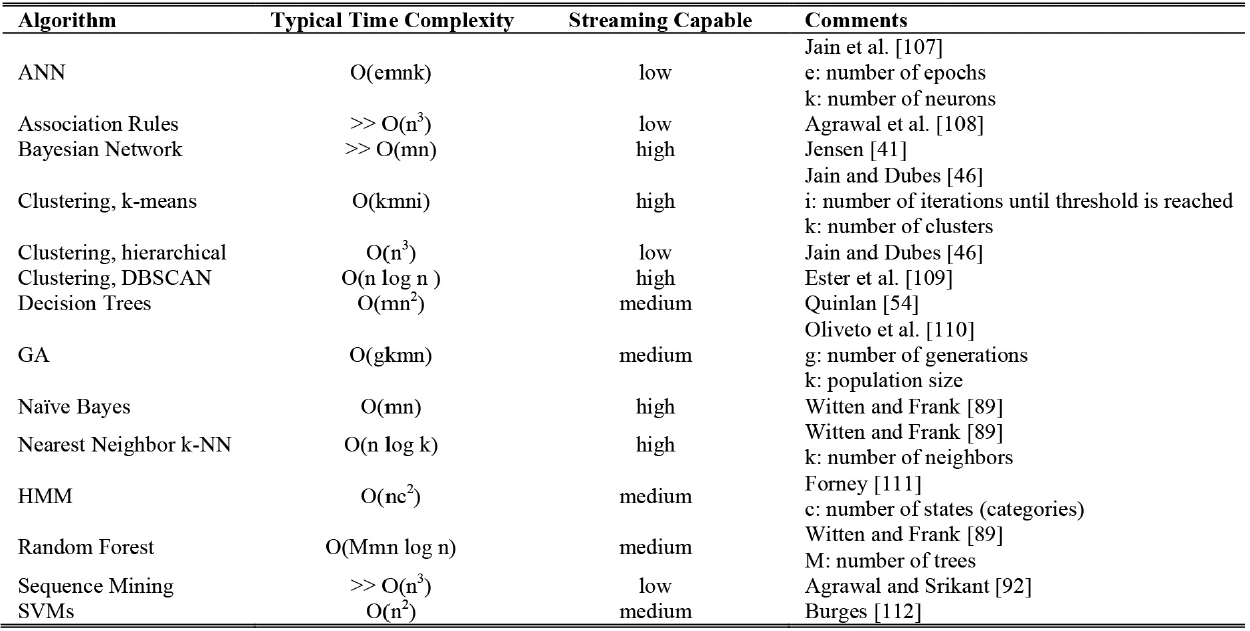
\includegraphics[width = \textwidth]{img/parts/introduction/Algorithm Comparison.png}
\end{table}

\subsection{Anomaly detection}

Novelty detection, also known as semi-supervised anomaly detection \citep{Scikit-learn-novelty_detection}, is the task of recognising data in the test set that differs in some respect to the data available during training. It is particularly useful when there is a large amount of "normal" data, but insufficient "abnormal" data. This is common in settings where measurements of a normal operating state are inexpensive to obtain, but generating a large amount of data in abnormal states is both difficult and costly. The goal is to train a model with what is considered to be "normal" data and then use that model to detect anomalies, \textit{i.e.} data not present in the training set. The techniques used should have a high detection rate, but with few false alarms, be scalable, and good time and space complexity. \cite{pimentel2014review} classified anomaly detection techniques into five categories: probabilistic, distance-based, reconstruction-based, domain-based, and information-theoretic.

\subsubsection{Probabilistic methods}

This approach is based on estimating the generative probability density function of the data, which is then thresholded in order to determine if a test sample originated from the same distribution or not. The estimation of the underlying data density from multivariate training data falls under two categories: parametric and non-parametric.\par

Parametric statistics assumes that the distribution of the population is known and is based on a fixed set of parameters \citep{IBM_ParatericStatistics}. The Gaussian distribution is commonly used for continuous variables, but more complex distributions may use mixture models such as \gls{gmm}. State-space models, often used in time-series data, assume that there are unobserved variables or parameters (states) that describe the evolution of the underlying system. Common state-space models used for novelty detection are the \gls{hmm} and the Kalman filter.\par

Non-parametric statistics makes no assumptions about the population's distribution or it's parameters. The use of kernel density estimators is an approach in which the probability density function is estimated using a large number of kernels distributed over the data space (\textit{e.g.} the Gaussian kernel).\par

Probabilistic methods are a mathematically well-grounded, effective, and transparent way to identify novel data as long as an accurate estimate of the data's probability density function has been obtained. However, this performance is limited when the training set is small. Non parametric approaches are usually preferred because prior knowledge of the data's distribution parameters is typically unavailable.

\subsubsection{Distance-based methods}

These methods determine the similarity between two observations based on distance metrics. Most methods are $k$-nearest neighbour- or clustering-based.\par

The $k$-nearest neighbours is a supervised algorithm that assumes that normal data points are close to each other, while anomalies are located far from these points. The Euclidean distance is a popular choice for distance measurement, and local density, in which the average of the $k$ nearest neighbours is considered, determines if a point is an anomaly or not.\par

The $k$-means clustering algorithm, a unsupervised algorithm, is a clustering-based method for identifying abnormalities. Here, data points from the training set are divided into clusters and classifying data points based on the cluster into which they are inserted.\par

Both $k$-nearest neighbours and clustering algorithms rely on the existence of a suitable distance metric to detect anomalies. Although they are very effective at this task, they do not scale very well to high dimensional datasets.

\subsubsection{Reconstruction-based methods}

Reconstruction methods attempt to model the underlying training data and classify the testing data based on it's reconstruction error. Both neural networks and subspace-based methods can be trained this way.

\subsubsection{Domain-based methods}

Domain-based methods attempt to define a boundary based on the training data, and testing samples are labelled based on their position relative to the boundary. \glspl{svm}, for example, generate a hyperplane that maximises the minimum distance to the closest point of either of the two classes. As for novelty detection, \glspl{svm} have been used in one of two ways: through the one-class approach, or through the support vector data description approach.\par

The aim of the one-class approach, introduced by \cite{scholkopf1999}, is to, though a kernel, separate all the data points from the origin and maximise the distance from this hyperplane to the origin. This does, however, require that a hyper-parameter corresponding to the percentage of data in the training set that is allowed to fall outside of this boundary.\par

The support vector data description method, proposed by \cite{tax2004} gives the training data a spherically shaped boundary with the minimum volume that encloses all, or most, of the data.\par

Although they are commonly used for anomaly detection, showing good performance, the kernel methods used can be computationally intensive. The choice of the appropriate kernel is also a challenge.

\subsubsection{Information-theoretic methods}

These methods attempt to detect novelties through significant changes in the information content of the data. Typical metrics include entropy, relative entropy, information gain, etc.
\chapter{State of the art}
\label{c:sota}

Intrusion detection is, as defined in \cite{Liao2013}, “the process of monitoring the events occurring in a computer system or network, and analysing them for signs of intrusions”. It can be deployed directly on the network node (host-based), where it monitors the activity for hosts containing sensitive information, or it can be deployed on the network (network-based), where it monitors traffic using sensors. Recent literature classifies the system’s detection approach as being either signature-, anomaly-, or specification-based \citep{Lokman2019}.

\section{Detection approaches}
\label{sec:ids_detection_approaches}

A signature-based \gls{ids} raises an alert when it finds a pattern in the network that corresponds to a signature in the system database. Its advantage comes from its simplicity, as it only requires a database of known attacks to compare network traffic to. However, this reliance on the attack signature database means that it will not recognise new attacks that are not stored there, meaning that regular updates are required.\par
The specification-based approach attempts to detect deviations from a protocol specification (well-defined rules that describe component behaviour). It is, again, a simple solution that requires only a set of rules that trigger an alert when not followed. Nonetheless, manually setting specifications is an error-prone and time-consuming task and must be adapted for different domains.\par
In the case of an anomaly-based \gls{ids}, an alert is raised when the network state deviates from what it considers to be normal behaviour. Here, the challenge relies upon defining what is considered normal behaviour, as a poorly defined model can generate alerts on what would otherwise be considered normal packets. A high rate of false positives could cause the user to ignore the alerts completely. Techniques for defining what constitutes normal behaviour include machine learning, packet frequency and statistical-based analysis, as well as a hybrid approach.\par
In the traditional desktop environment, a hybrid approach is a combination of several \gls{ids} techniques, such as network- and host-based \gls{ids}. Here, the host-based \gls{ids} aggregates information into a standard format, which is then transmitted to the network-based \gls{ids}, where it is aggregated and processed. In the case of anomaly detection in \gls{can}, a hybrid-based approach consists of the combination of more than one detection method, considering various packet features, e.g., ID field, payload, timing interval and frequency.

\section{IDS evasion techniques}

Intrusion detection systems are commonly used in many networks, and attackers have adapted in order to avoid being detected. Evasion techniques mostly make the use of fragmentation, flooding, obfuscation and encryption.\par
Fragmentation is the process of dividing a packet into smaller packets, which are then reassembled when received. To analyse these fragmented packets, an \gls{ids} is required to re-assemble them. Attackers then take advantage of fragmentation overlap, overwrite and timeouts to escape detection. Flooding occurs when an attacker overwhelms the detector with a massive stream of packets, which causes it to fail. Obfuscation works by making a message difficult to understand, typically by changing the code while maintaining its functionality. This reduction in the code readability makes both static analysis and reverse engineering much more difficult. An \gls{ids} using a signature database will also see a decrease in its ability to detect attacks. Although encryption offers many security benefits, attackers can also leverage it to their advantage. Attacks on encrypted protocols, for example, cannot be detected by an \gls{ids} that relies on a signature database, as it cannot interpret the packets contents \citep{Khraisat2019}.

\section{Intrusion detection in the Controller Area Network}
\label{sec:can_ids}

Although \glspl{ids} are commonplace in traditional IP networks, they are still being developed for use in vehicles, more specifically in the \gls{can} bus. Therefore, there still is no single best approach, but multiple different attempts to build a reliable \gls{ids}.

\subsection{Based on packet frequency}

\cite{taylor2015frequency} proposed a frequency-bases analysis of network traffic flow in order to detect anomalies. Through the use of a \gls{ocsvm}, they found that they were able to identify when packets were artificially inserted or removed by the mean-time interval between packets of the same ID. Another frequency-based detection method was proposed by \cite{song2016intrusion}, in which they recorded no false positives during the packet injection tests.\par
An \gls{ids} that is based on the offset ratio and time interval between request and response was proposed by \cite{lee2017otids}. The system periodically sends remote frame requests and analyses the response time, and attacks were successfully identified because of the abnormalities in the instant reply ratio, lost reply ratio, correlation coefficient between offsets and time intervals, and average response time.\par
A clock-based \gls{ids} was developed by \cite{cho2016fingerprinting}, where it identified \glspl{ecu} based on the intervals of periodic messages. This baseline then allowed for the detection of abnormal behaviour in the network, with a reported false positive rate of 0.055\%. Unlike most \glspl{ids}, it also facilitated the identification of the misbehaving \gls{ecu}.

\subsection{Based on network entropy}

An entropy-based anomaly detection mechanism was proposed in \cite{muter2011entropy}. Here, the developed \gls{ids} analysed variation in the network entropy (\textit{i.e.}, how much coincidence a given dataset contains) to detect anomalies. Through increased message frequency, message flooding, and simulation of unrelated events, they concluded that "deviations from the normal behavior of in-vehicle networks can successfully be identified by an information-theoretic detection approach". Another entropy-based system was proposed by \cite{marchetti2016evaluation}, in which they claimed that this represents a "viable approach for identifying CAN bus anomalies caused by the activity of attackers that [are] injecting messages over the CAN bus". However, limitations include only being able to detect attacks where packets are inserted at a high rate.

\subsection{Based on network data probability}

\cite{kang2016intrusion} used probability-based feature vectors extracted from the network packets to train a \acrlong{dnn}. The training was performed offline, while the detection was done against incoming packets in the network. They achieved a 99\% detection racio against a \gls{tpms} spoofing attack. Another deep learning model was presented in \cite{Taylor2016}, in which the authors developed an \gls{lstm} that attempts to predict the next data word originating from each sender on the bus, flagging anomalies. However, it worked only for a single CAN ID and did not support online learning.\par
In \cite{narayanan2016obd_securealert}, the authors proposed the utilisation of a \gls{hmm} to model what is considered normal vehicle function. The \gls{ids} works by signalling low probability changes of state (like a sudden jump from 25 kph to 160 kph) as an anomaly. The system was able to detect the introduction of anomalous RPM data, and they state that advantages of this approach include the fact that it can be applied in a plug-and-play fashion to both new and older vehicles.

\subsection{Hybrid}

\cite{weber2018embedded} presented a hybrid anomaly detection system that combines both specification-based detection and machine learning, drawing from the advantages of both. In a first stage, static checks are made, and then the machine learning part applied learning checks for temporal analysis of the \gls{can} packets.\par
A \gls{htm} model was developed by \cite{wang2018distributed}. This is a memory-based model that is capable of online learning, meaning that it can continuously learn with new \gls{can} data. Results from packet insertion and modification attacks show that it outperforms existing \gls{can} \glspl{ids} that used \gls{rnn} and \gls{hmm} models.

\subsection{Based on protocol specifications}

\cite{larson2008approach} investigated the use of a specification-based \gls{ids} with security rules derived from the e \gls{can} v2.0 and CANopen draft standard 3.01 communication protocol and object directory sections. These enforce the correct functioning of the protocol according to specification, signalling deviation from the rules as anomalous traffic. They tested six types of attacks (spoof, replay, read, modify, flood, and drop), concluding that most attacks can be readily detected and that "both protective and detective measures will be required in future in-vehicle networks".

\subsection{Based on attack signatures}

To act as attack signatures for \gls{ids}, \cite{muter2010} designed eight anomaly detection sensors that were generated from \gls{can} bus system characteristics. The signatures created in the sensors included \gls{can} bus protocol specifications, which described permitted packets with regard to the intended communication bus system, specifications of packet payload that complied with data range, and approved packet frequency and interval behavior, among others. According to the overall findings, the sensors were able to identify abnormalities with no false positive alert. The approach, however, was unable to identify packet insertion attacks that complied with the \gls{can} specification's usual behavior.\par
Finite-state automata were used by \cite{studnia2018} to extract the attack signatures derived from conventional \gls{ecu} specifications in order to detect an abnormal sequence of \gls{can} packets. The attack packets were simulated using altered CAN frames while the authors tested the suggested approach using malicious packet injection. However, as it emitted the initial frames of the broadcasted attack packets, the detection performance of the approaches became useless even if they could detect deviations from the typical states of CAN activity.

\section{Challenges for automotive}

There are, however, several challenges that must be overcome to successfully implement an \gls{ids} in a \gls{can} bus. First, most \glspl{ecu} have very limited resources, meaning low memory capacity, computational power, and data transmission rate. Another consideration is the time-sensitive nature of the packets being transmitted \citep{hoppe2009applying}. Proper vehicle function must be maintained, which means that \gls{can} packets must be managed in real-time. Otherwise, the safety of the driver might be at risk, as there would be an additional delay in information processing. Typical \gls{ids} solutions were developed for conventional Internet Protocol (IP) networks. As this environment is very different from the in-vehicle one, adopting existing solutions is not possible. The nature of the vehicle environment is also a constantly moving one, and at various speeds. This means that an \gls{ids} must have a certain degree of autonomy, as establishing a connection to an outside party may not always be possible. Lastly, it must be an efficient solution, both in terms of cost, for it to be implemented in mass-production, and its physical aspects, i.e., not requiring massive amounts of rewiring, as it may be infeasible for manufacturers \citep{Lokman2019}.\par
In a traditional IT setting, a system administrator is usually in charge of maintaining the system functioning properly and up to date and is also the one notified in case of an alert. In the automotive domain, however, the \gls{ids} cannot be maintained by a qualified administrator, and a typical user cannot be expected to be an IT expert. This means that tasks like maintenance and alert handling can be delegated to him in a limited way. This might motivate the design of the system to be as autonomous as possible, but the high safety requirements of automotive systems make this a challenging task. The authors of \citep{hoppe2009applying} state that "in general, automotive systems shall never take safety relevant decisions autonomously but may only support the driver in his reaction (final decisions regarding control or safety of the vehicle are only to be made by the driver)". Because of this, special care must be taken when deciding upon the way of communicating an alert to the driver. This communication must be done in a modern way, taking advantage of the car's multimedia system, and must not cause panic. If a driver reaction is required, it is advantageous to provide suggestions and the need to disrupt the driver must be kept to a minimum. They identified four aspects that should be taken into consideration when designing a way to communicate an alert to the driver: the use of a modern way of communicating, transmitting a sense of peace of mind, avoiding repetition, and support of the driver's decision-making. They then propose a three-stage model, which can be seen in Figure \ref{fig:ids_adaptive_dynamic_reaction} for alert communication to the driver depending on the severity of the intrusion. The three stages are visual, containing elements like the dashboard or central screen, acoustic, through the vehicle's sound system, and haptic, through force feedback in the brake pedal or steering wheel.

\begin{figure}
    \centering
    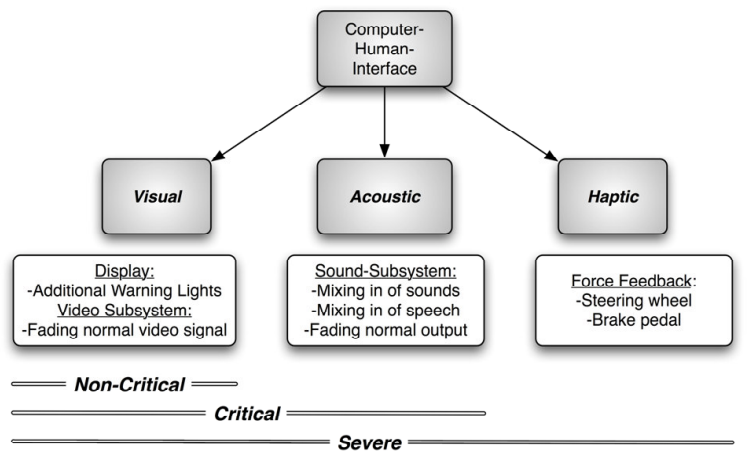
\includegraphics[width = \textwidth]{img/parts/app/Adaptive IDS Alarm System.png}
    \caption{Three stages model for IDS alert communication \citep{hoppe2009applying}}
    \label{fig:ids_adaptive_dynamic_reaction}
\end{figure}

Increasing severity is implicated by going from visual to acoustic and then to haptic. A visual-only message is used for non-critical alarms as the driver may not immediately look at the visual indication. Combining visual with acoustic signals indicates a critical alarm, as the driver would be immediately alerted. Haptic signals, like steering wheel vibration, are reserved for only severe alarms as they might frighten the driver. However, communication ability increases by going from haptic to acoustic and then to visual. Haptic signals are only able to indicate that something is wrong, without further information. Audible signals can provide more context, with visual messages informing the driver about what is the problem.\par
The severity of the alarm, however, is not the only factor to determine what stage should be used. Environmental context gathered from the vehicle's multiple sensors may aid in this decision. If the light sensors, for example, detect a high level of brightness, the system may opt for audiovisual indication in a non-critical situation, as a visual-only warning would be difficult for the driver to notice.

\part{Core}
\chapter{Contribution}
\label{c:contribution}

Many intra-vehicle \gls{ids} approaches have been studied, as shown in \ref{sec:can_ids}, but they have mostly relied on a few labelled datasets such as \cite{CANDataset_Car-Hacking}. Here, the proposed system aims to be an \gls{ids} based on unsupervised machine learning for anomaly detection that makes decisions based on the statistical and information-theoretic characteristics of network traffic gathered in real-time. In other words, the system is able to learn what constitutes normal traffic, and signal when it detects behaviour that it considers to be novel. This would allow manufacturers to deploy the \gls{ids} in a plug-and-play fashion, without having to tune it for every different configuration of the vehicle.
\chapter{Datasets}
\label{c:datasets}

Various datasets were used in the development of this \gls{ids} prototype, including publicly available datasets obtained from both a real environment and synthetically generated, as well as datasets generated for the purpose of this prototype's development. These are described below.

\section{Car Hacking dataset}

These datasets were generated as part of the study published by \cite{Song2020}. Traffic was collected from a Raspberry Pi connected to a real vehicle via the OBD-II port, while another Raspberry Pi was used to inject traffic. The vehicle was parked with the engine turned on throughout the data gathering process. Five datasets were produced, with an overview of the attack datasets being available on Table \ref{tab:car_hacking_dataset_overview}.

\begin{itemize}
    \item Normal: An attack-free dataset
    \item \gls{dos} attack: Packets with the ID set to 0 were injected every 0.3 ms, impairing network availability
    \item Fuzzy attack: Packets with random IDs and payloads were injected every 0.5 ms, aiming to cause vehicle malfunction
    \item Gear spoofing attack: Packets a specific ID and payload were injected every 1 ms, successfully changing the gear value on the instrument panel
    \item RPM spoofing attack: Packets a specific ID and payload were injected every 1 ms, successfully changing the RPM gauge on the instrument panel
\end{itemize}

\begin{table}
    \centering
    \begin{tabular}{*{3}{c}}
        \toprule
        \textbf{Attack type} & \textbf{Normal messages} & \textbf{Injected messages}\\
        \midrule
        DoS Attack & 3,078,250 (84\%) & 587,521 (16\%)\\
        Fuzzy Attack & 3,347,013 (87\%) & 491,847 (13\%)\\
        Gear Spoofing & 2,766,522 (82\%) & 597,252 (18\%)\\
        RPM Spoofing & 2,290,185 (78\%) & 654,897 (22\%)\\
        \bottomrule
    \end{tabular}
    \caption{Car Hacking dataset overview}
    \label{tab:car_hacking_dataset_overview}
\end{table}

\section{IEEE Car Hacking: Attack \& Defense Challenge 2020}

The datasets published by \cite{kang2021car} were created to be used in the Car Hacking: Attack \& Defense challenge. It had two rounds: preliminary and final. For the preliminary round, training and submission datasets were provided, both containing driving and stationary vehicle traffic. For the final session, a single dataset with multiple attacks was created.\par
An overview of the preliminary datasets can be seen on Table \ref{tab:ieee_challenge_dataset_overview}. For both driving and stationary scenarios, the datasets contained flooding, spoofing, replay, and fuzzing attacks. Attack-free datasets were also provided.

\begin{table}
    \centering
    \begin{tabular}{*{7}{c}}
        \toprule
        \textbf{Purpose} & \textbf{Status} & \textbf{Flood} & \textbf{Spoof} & \textbf{Replay} & \textbf{Fuzzy}\\
        \midrule
        \multirow{4}{*}{Training} & \multirow{2}{*}{Driving} & 77,373 & 3,879 & 23,775 & 45,474\\
        & & (4.1\%) & (0.2\%) & (1.3\%) & (2.4\%)\\
        & \multirow{2}{*}{Stationary} & 76,807 & 3,877 & 23,818 & 44,405\\
        & & (4.3\%) & (0.2\%) & (1.3\%) & (2.5\%)\\
        \midrule
        \multirow{4}{*}{Submission} & \multirow{2}{*}{Driving} & 96,559 & 22,489 & 37,869 & 44,770\\
        & & (4.8\%) & (1.1\%) & (1.9\%) & (2.2\%)\\
        & \multirow{2}{*}{Stationary} & 95,120 & 20,094 & 25,012 & 51,923 \\
        & & (5.4\%) & (1.1\%) & (1.4\%) & (3.0\%)\\
        \bottomrule
    \end{tabular}
    \caption{IEEE Car Hacking: Attack \& Defense Challenge 2020 dataset overview}
    \label{tab:ieee_challenge_dataset_overview}
\end{table}

\section{Automotive Controller Area Network (CAN) Bus Intrusion Dataset v2}
\label{subsec:tue_dataset}

The datasets made available by \cite{Dupont2019} consists of bus data from an Opel Astra, a Renault Clio, and a custom built prototype. For all three systems, attack-free datasets were provided along with datasets containing diagnostic, fuzzing, replay, spoofing and \gls{dos} attacks.

\section{CrySyS Lab}
\label{sec:dataset_crysys}

This dataset was obtained from \cite*{crysys} and consists of CAN traffic collected from 25 minutes of driving in the highway as well as in small streets. A variety of packet modification attacks were simulated using the tool publicly available in \cite*{infector}, which allows for easy modification of CAN log files. These attacks consist of modifying the payload of packets with a given ID, akin to a man-in-the-middle attack. Five attack datasets were generated, along with the attack-free version, and the attacks target the payload of the packets with ID 120 starting at 50\% and ending at 90\% of the total file. The attacks consist of holding the payload at a constant value, modifying the payload to be a random value, adding an increasing amount to the original payload, decreasing the payload from 255 to 0 and repeating, and adding a delta of 1000 to the original payload. Unlike other datasets, were packet insertion is performed and the attack can mostly be detected via the interval between arriving packets, these attacks do not insert any packets. Attacks can only be detected by observing anomalies in the behaviour of the payloads.

\section{CES}

The setup used to generate real CAN traffic can be seen on Figure \ref{fig:setup}. It is composed of various real vehicle ECUs, along with a modern touchscreen, and a Raspberry Pi to capture CAN traffic and running the IDS here proposed. Three attacks were simulated (fuzzing, flooding, and spoofing) by inserting packets every 200ms. The following unlabelled datasets were generated:

\begin{itemize}
    \item Baseline: 2,508,370 packets of attack-free traffic.
    \item Fuzzy attack: 184,833 packets containing two instances of a fuzzing attack.
    \item Denial-of-Service attack: 235,187 packets containing two instances of a Denial-of-Service attack.
    \item Left blinker spoofing attack: 375,569 packets containing two instances of a spoofing attack targeting the left blinker signal.
\end{itemize}

\begin{figure}
    \centering
    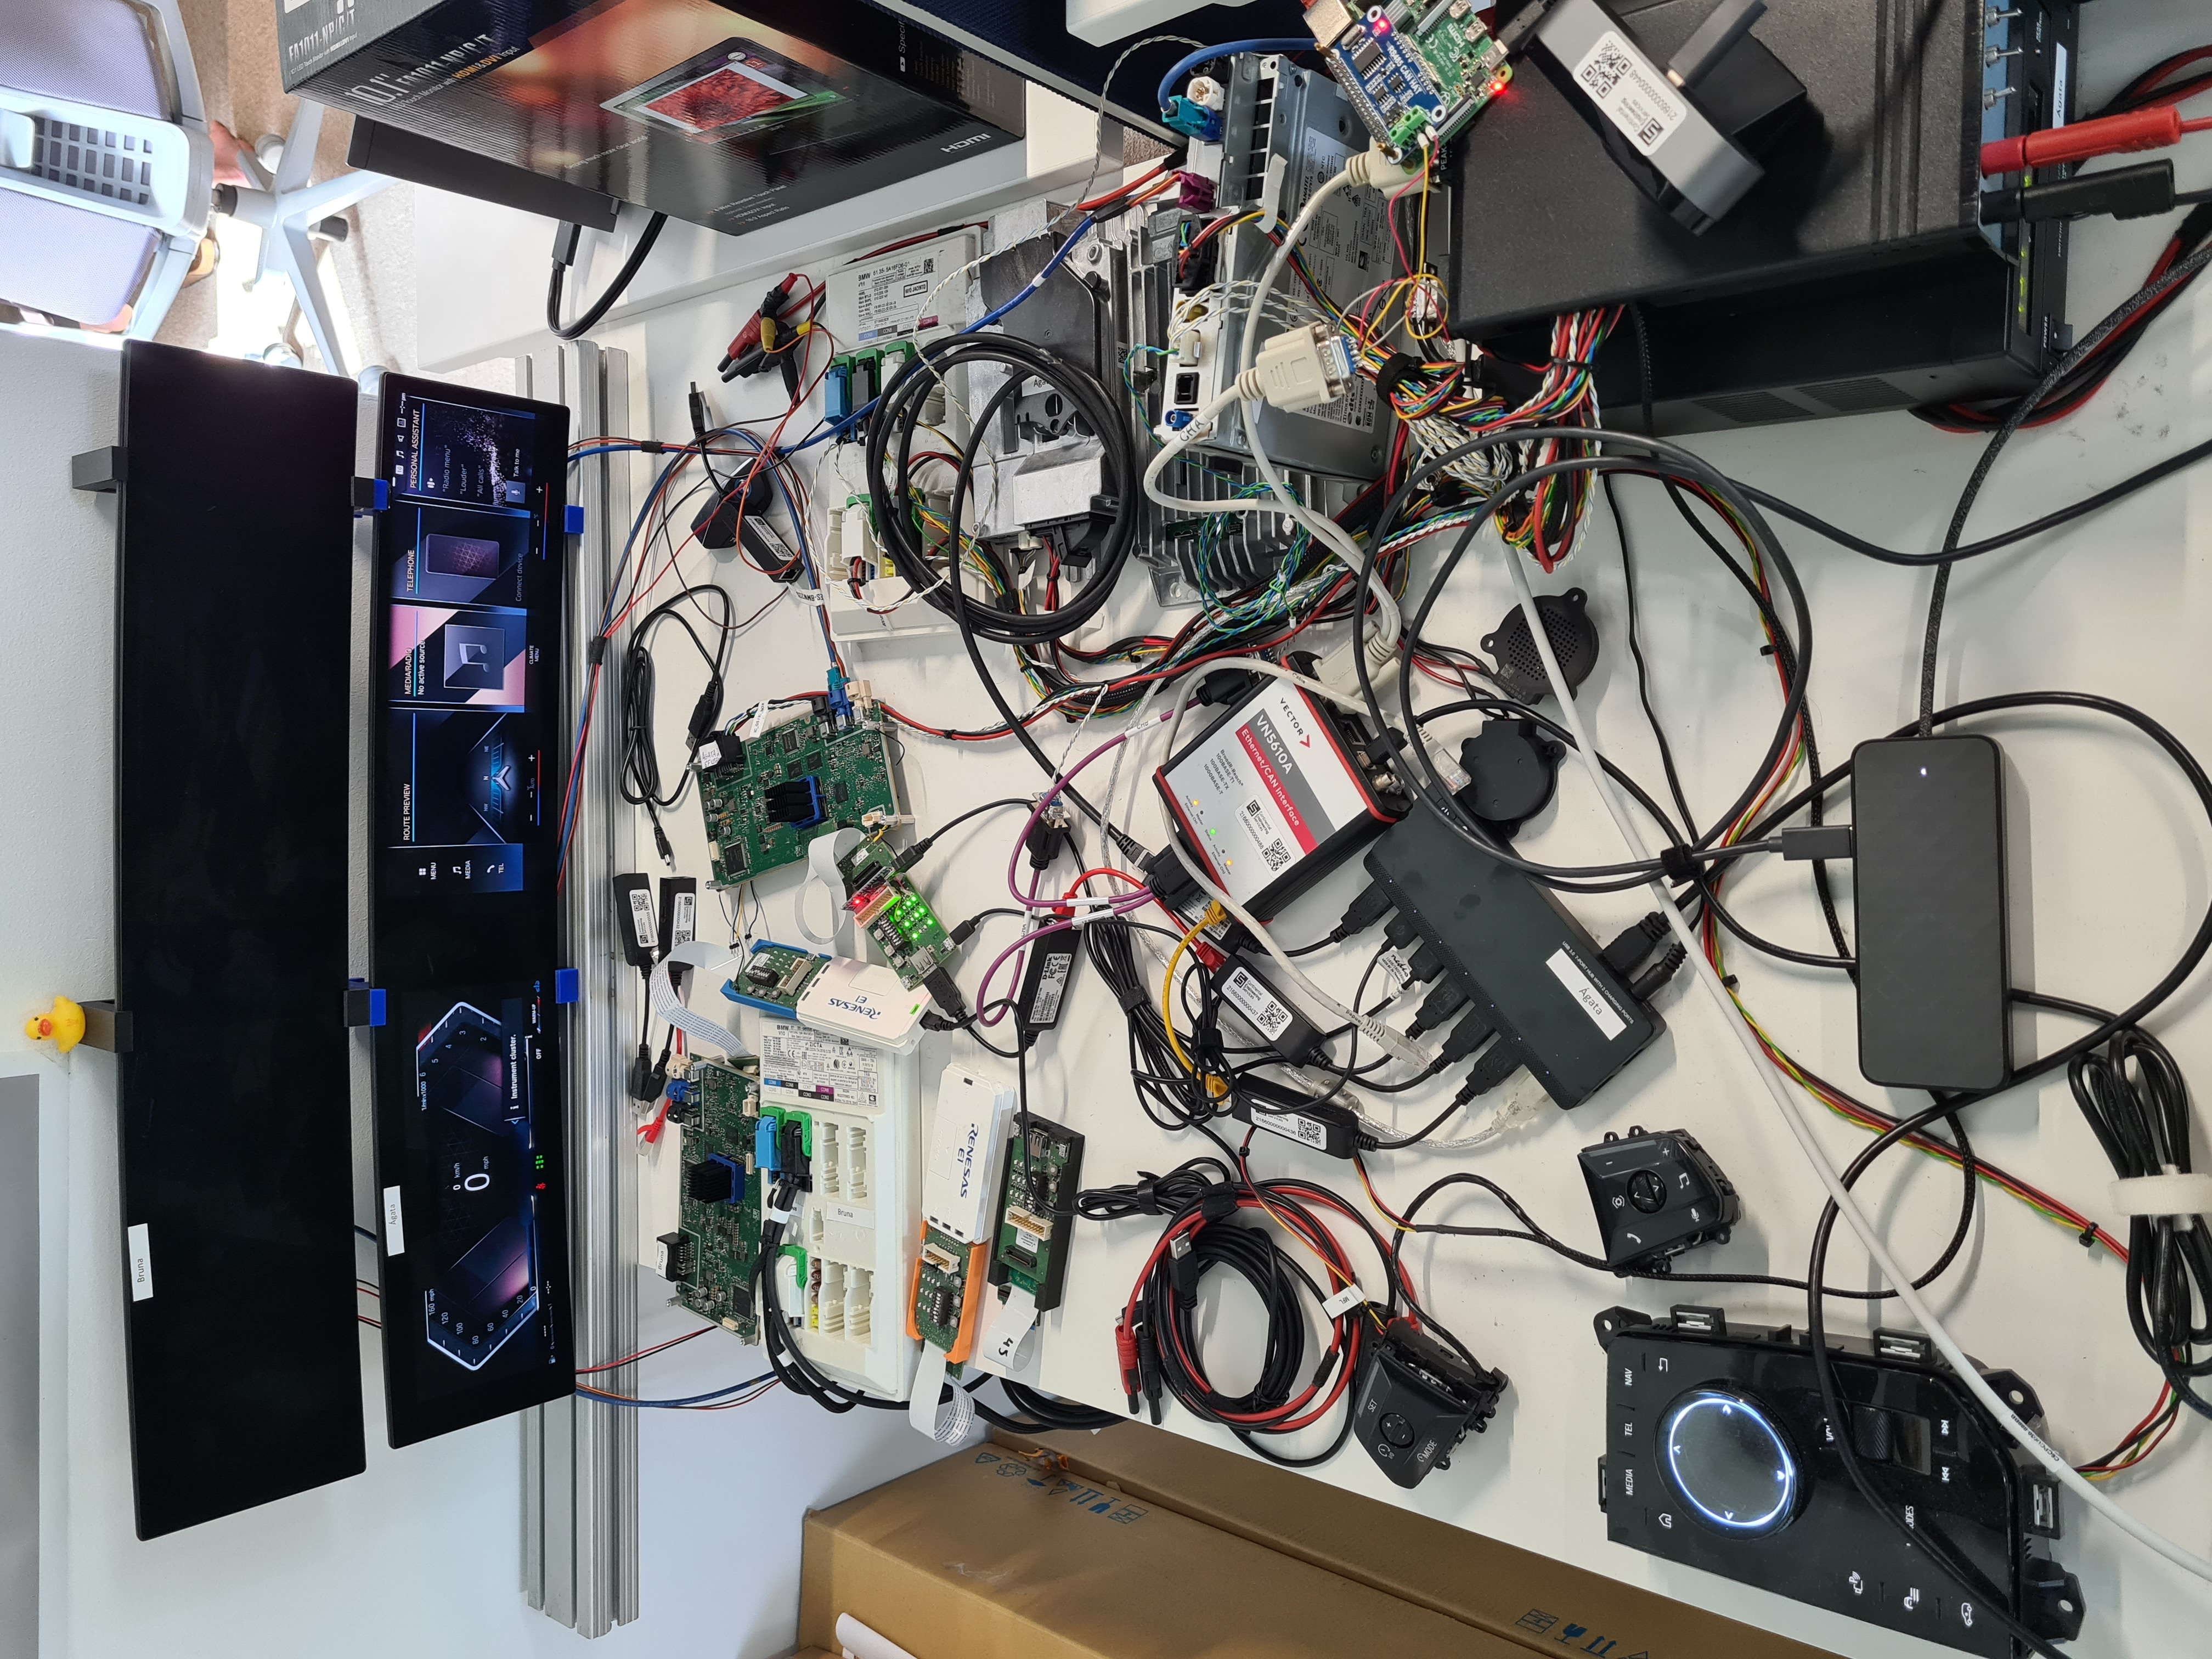
\includegraphics[angle = -90, origin = c, width = .3\linewidth]{img/parts/app/Setup.jpg}
    \caption{Setup used to generate real CAN traffic}
    \label{fig:setup}
\end{figure}
\chapter{Application}
\label{c:application}

This chapter covers the proposed solution and its implementation. In Section \ref{sec:app_architecture}, the overall system is explained, including how feature extraction is performed as well as how the model is trained. Section \ref{sec:app_training} goes into more detail on how the trainig mechanism works. The features used to train the model, and their selection process, are documented in Section \ref{sec:app_features}. In Section \ref{sec:app_embedded}, the system's implementation in an embedded environment is detailed, along with its behaviour regarding resource restriction. Finally, Section \ref{sec:app_exe} shows the application's \gls{cli} and visual interface. The application's full documentation is available in Appendix \ref{apdx:sec:code_documentation}.

\section{IDS architecture}
\label{sec:app_architecture}

In \ref{sec:ids_detection_approaches}, various approaches to \gls{ids} deployment were presented, most notably its placement (host or network-based) and detection techniques (signature, specification, anomaly, or hybrid). Here, a host-based \gls{ids} for anomaly detection is put forward. Instead of the \gls{ids} residing in a separate \gls{ecu} connected to the network, the \gls{ids} is deployed on all of the vehicle's \glspl{ecu}. It then monitors the same messages as the \gls{ecu} in which it is deployed. Since it would be present on all \glspl{ecu}, an attack on any relevant message ID would, theoretically, trigger at least one alarm. Monitoring a small set of IDs also aids with detection because an anomaly in the behaviour of a certain ID becomes more noticeable in the average of the set when compared to a larger number of IDs being monitored.\par
Features are extracted from a rolling window with an overlap of 75\% between consecutive windows. Given the same amount of packets, this allows for the extraction of a larger amount of features during the training phase, when compared to non-overlapping windows.\par
A diagram of the overall system can be seen in Figure \ref{fig:ids_architecture}.

\begin{figure}
    \centering
    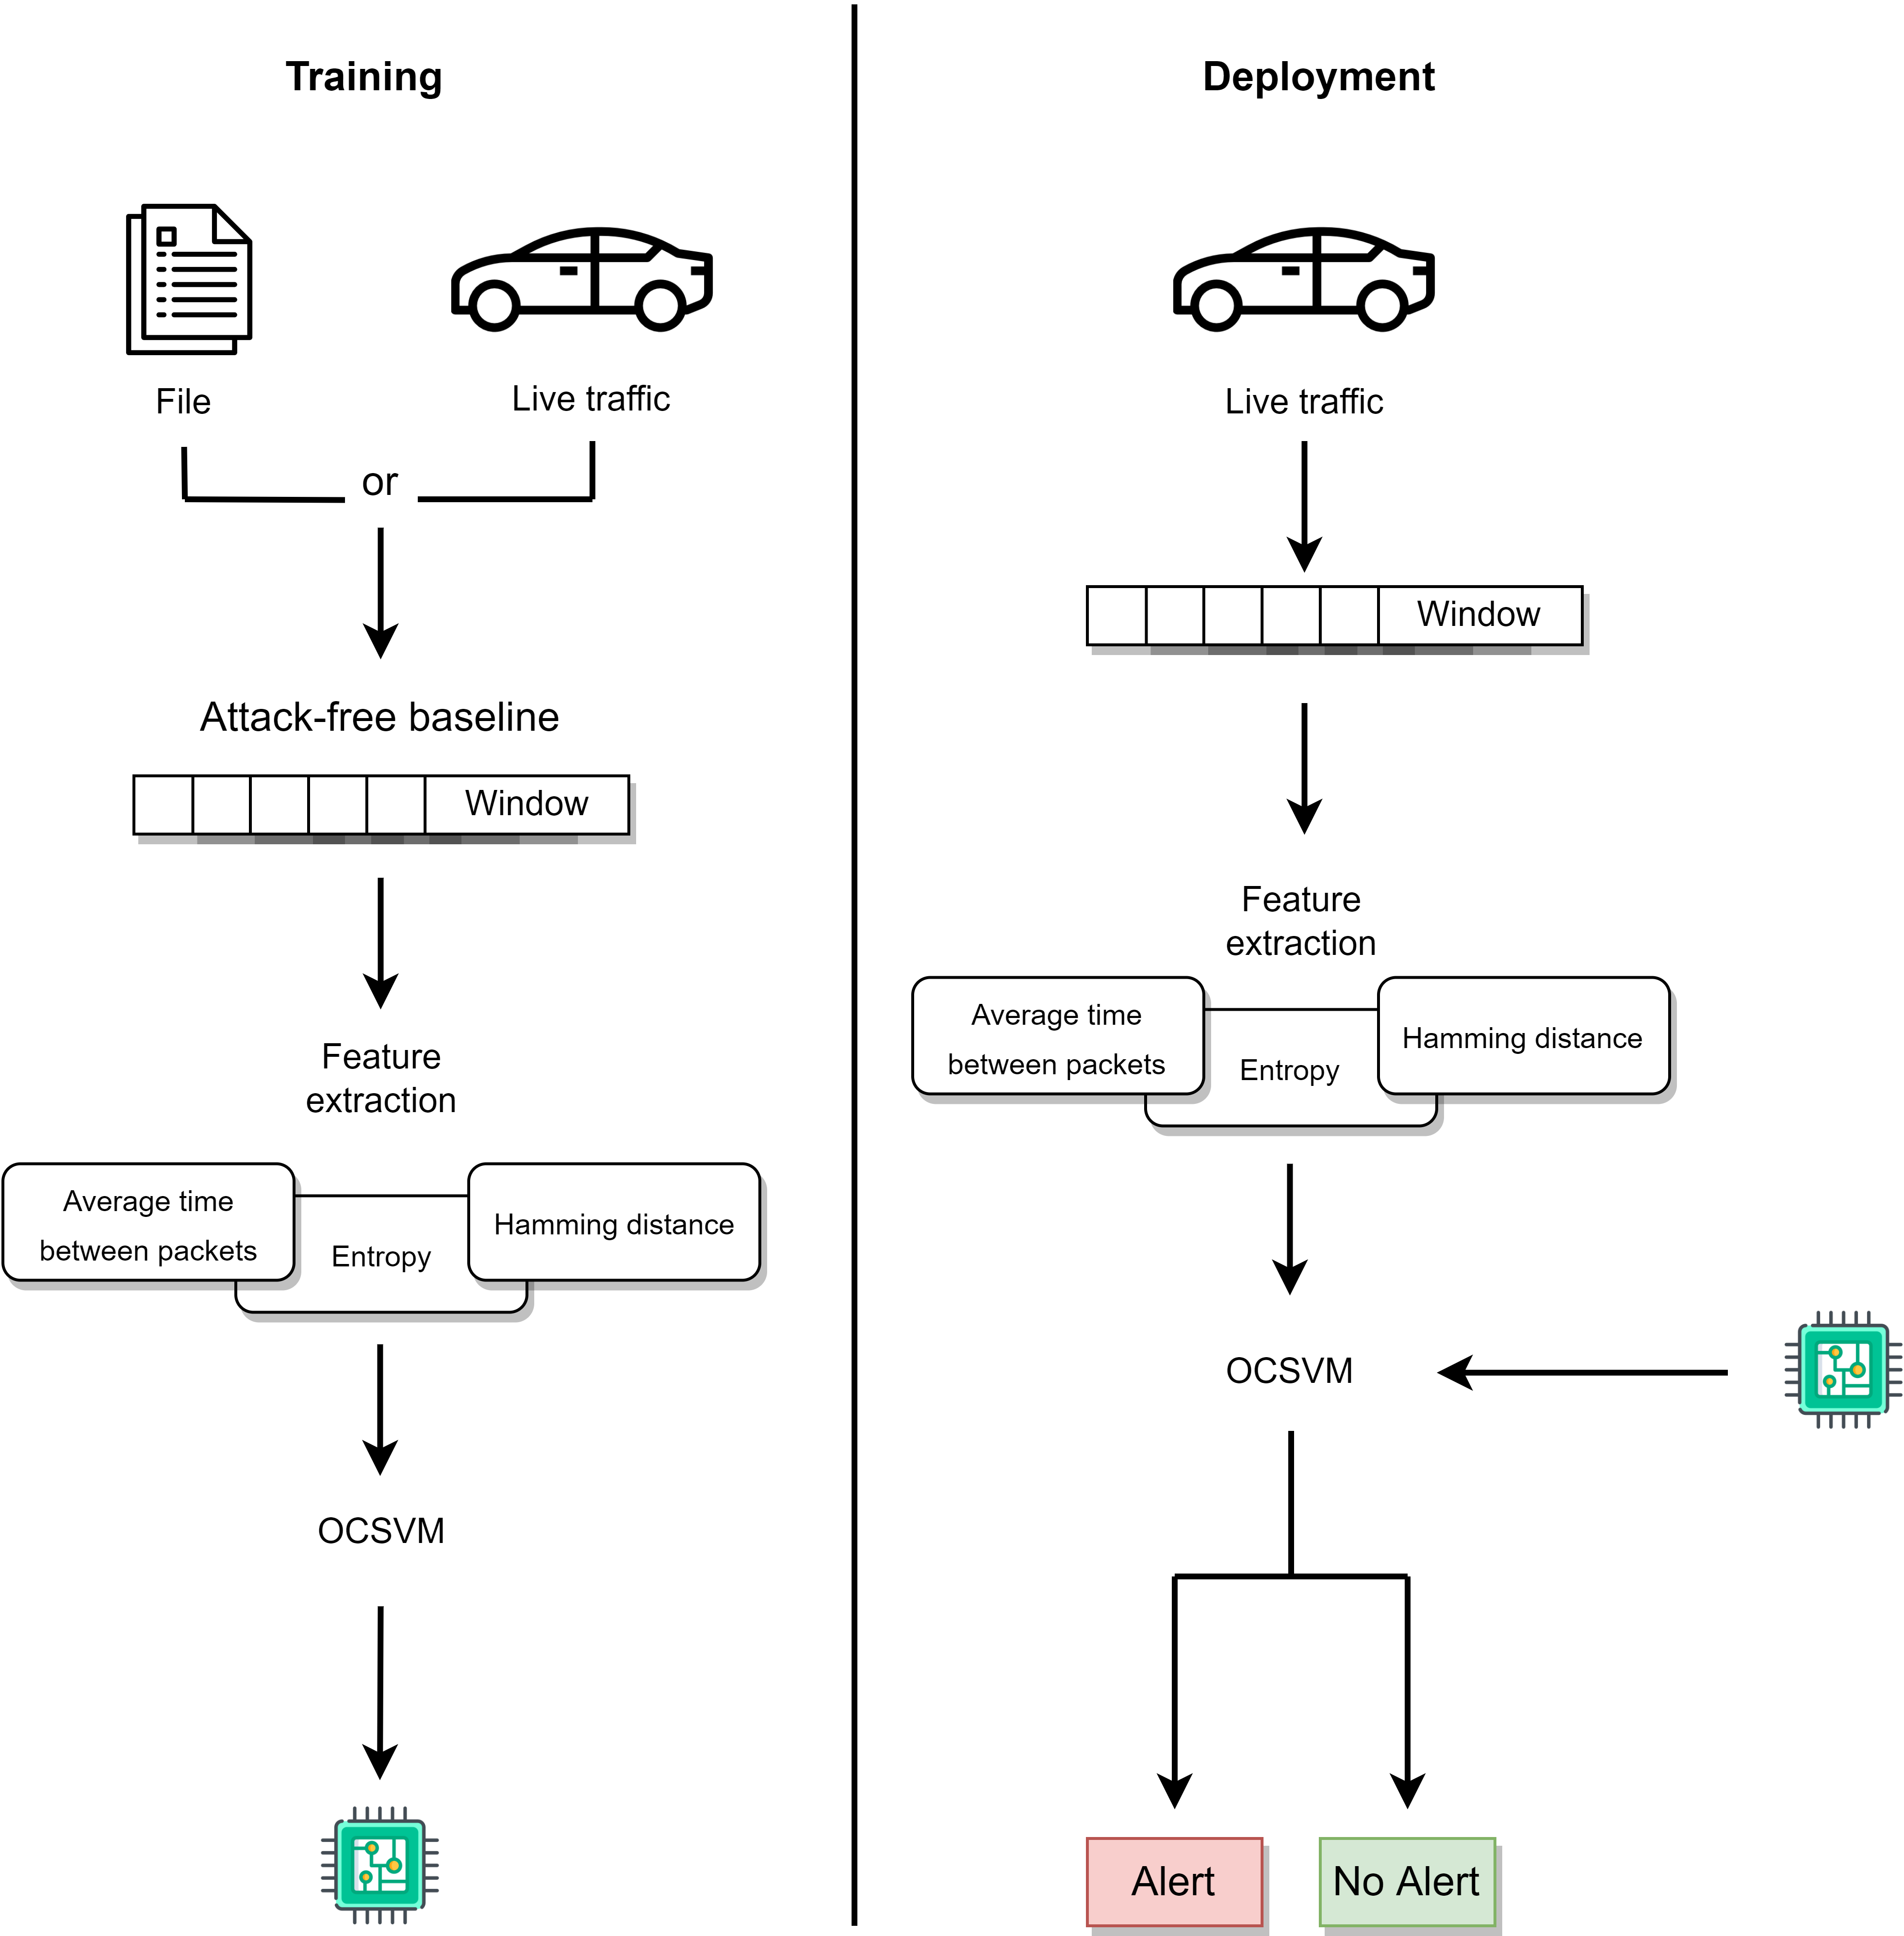
\includegraphics[width = \textwidth]{img/parts/app/IDS.png}
    \caption{IDS architecture}
    \label{fig:ids_architecture}
\end{figure}

\section{Training}
\label{sec:app_training}

Training the \gls{ids} can be done both in an online and offline fashion. Training online means that a baseline reading is gathered from live traffic, which must be attack-free to generate an accurate model because attacks are detected based upon significant deviations from the baseline traffic's characteristics. Offline training is done by providing the \gls{ids} with a \gls{csv} file containing CAN traffic that will serve as a baseline.\par
Features are extracted using a rolling window on the collected traffic, which are then scaled to fit in the [0, 1] interval. The minimum and maximum values of each feature are saved to perform proper feature scaling when the \gls{ids} is deployed.\par
The kernel method is employed using the Gaussian kernel with $\epsilon = 1$ and the model is trained with the $\nu$ parameter set to 0.01. The \gls{ids} is then saved to the filesystem so it can be recovered upon a system restart. The documentation for the structure and training function can be seen in Figures \ref{fig:ids_struct} and \ref{fig:ids_train}, respectively.

\begin{figure}
    \centering
    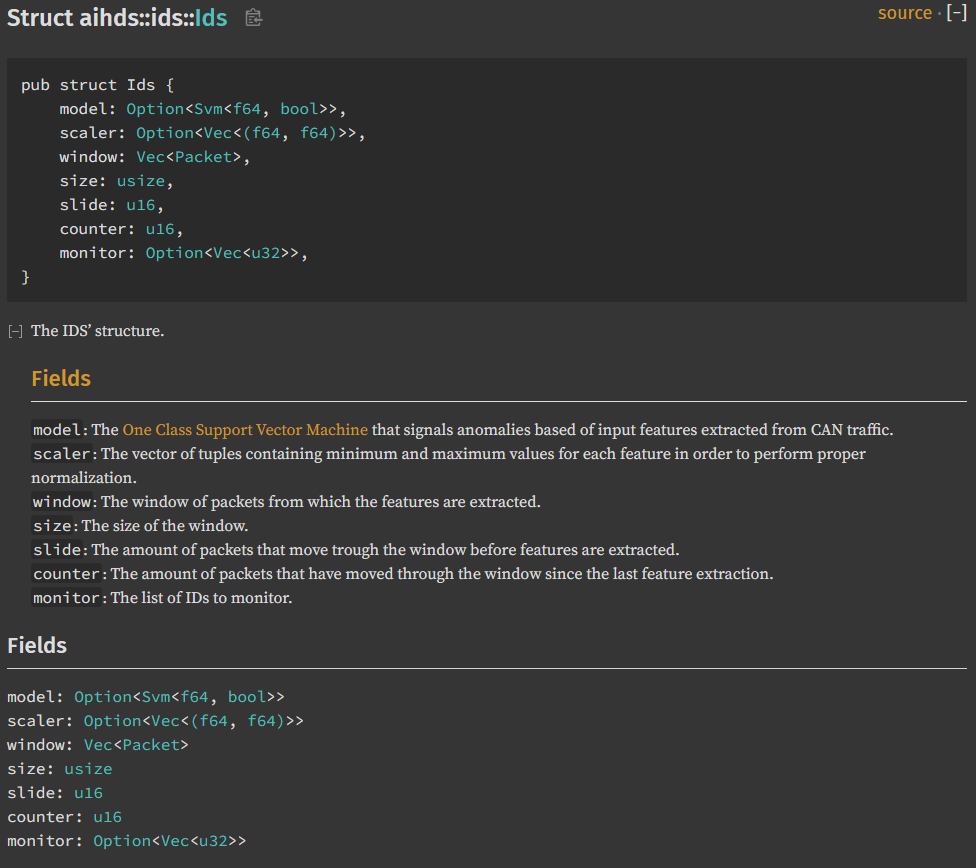
\includegraphics[width = \linewidth]{img/parts/docs/ids/ids_struct.png}
    \caption{\gls{ids} structure}
    \label{fig:ids_struct}
\end{figure}

\begin{figure}
    \centering
    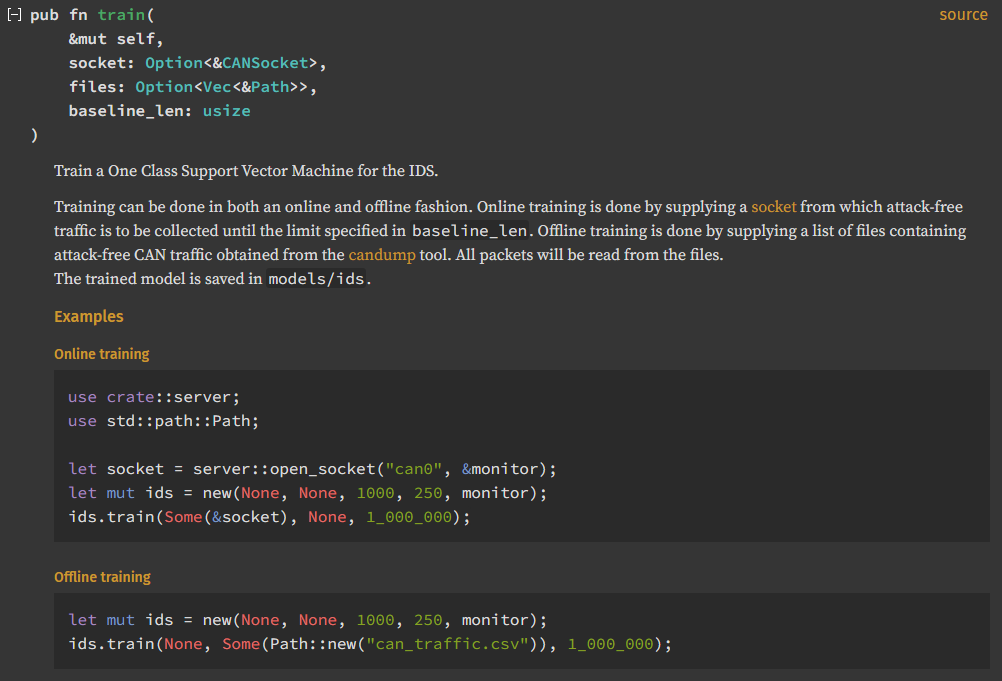
\includegraphics[width = \linewidth]{img/parts/docs/ids/ids_struct_train.png}
    \caption{Training function}
    \label{fig:ids_train}
\end{figure}

% \begin{itemize}
%     \item \textit{model}: The \gls{ocsvm}
%     \item \textit{scaler}: A vector of tuples containing the minimum and maximum values of each feature from the baseline
%     \item \textit{window}: The collection of packets from which features are extracted
%     \item \textit{size}: The amount of packets the window can hold
%     \item \textit{slide}: The amount of packets that leave and enter the window in a FIFO fashion
%     \item \textit{counter}: The number of packets that have left and entered the window between slides
%     \item \textit{monitor}: The collection of IDs to monitor
% \end{itemize}

\section{Features}
\label{sec:app_features}

This section focuses on the features extracted from \gls{can} bus traffic that are then used as input to the \gls{ocsvm} model. Prior research on \glspl{ids} that focus on \gls{can} has found success in the use of frequency analysis and information-theoretic algorithms, as shown in Section \ref{sec:can_ids}. Frequency analysis was one of the first methods used to detect packet insertion attacks. Since many packets of the same ID are sent at a consistent interval (typically 10 or 20 milliseconds), a variation of these timings caused by a bad actor inserting packets into the network would be picked up as an anomaly. On the other hand, information-theory may aid in detecting anomalous behaviour caused by packet modification attacks, or packet low-frequency packet insertion.\par
Here, the proposed features are described, and the feature selection process is presented.

\subsection{Packet frequency}

Frequency analysis consists of measuring the average time between consecutive packets with the same ID. Since many packets sharing the same ID are sent at regular intervals, an attacker inserting new packets into the network would decrease the time between packets, which would be detected by the \gls{ids}. Likewise, packet suppression would also trigger an alert.\par
Calculating the arrival time between packets can done by \[T(p_{t_0}, p_{t_1}) = t_1 - t_0\] where $t_0$ and $t_1$ are consecutive arrival timestamps for packets of the same ID.

\subsection{Shannon entropy}

In the \gls{can} domain, traffic is more restricted than in standard computer networks. This means that, generally, entropy in an automotive network is lower \citep{muter2011entropy}. If an attacker replaces the payload of a given ID, it likely would change the network entropy, triggering an alert (an instance of this would be a constant payload on an ID that usually sends distinct values, or vice-versa).\par
The concept of information entropy was first introduced by \cite{shannon1948}. Shannon entropy is often defined as being the amount of information or uncertainty of a random variable. For an alphabet $X$, and a random variable $x \in X$ distributed according to $p: x \rightarrow [0, 1]$, Shannon entropy is defined as \[H(X) = - \sum_{i - 1}^{n} P(x_i) \log_2 P(x_i)\]\par
An occurrence with probability 1 has no entropy, while a set of occurrences with a balanced probability distribution has an entropy value of 1. 

\subsection{Hamming distance}

In information theory, the number of points where the matching symbols are different between two strings of equal length is known as the Hamming distance \citep{hamming1950}. For example, the Hamming distance between 0000 and 1111 is 4, while the Hamming distance between 0101 and 1101 is 1. The formula for evaluating the Hamming distance between two words of length $k$ is \[H_d(x, y) = \sum_{i = 1}^{k} \vert x_i - y_i \vert\]\par

Here, the proposed approach consists on calculating the Hamming distance between consecutive packets in the network, similar to what was proposed by \cite{stabili2017}. The authors formulated this as being \[H_d(p_t, p_{t + 1}) = \sum_{i = 1}^{k} p_{t}^{i} \otimes p_{t + 1}^{i}\] where $p_t$ is a generic payload at time $t$ and $p_t^i$ is the $i_{th}$ element of that payload.

\subsection{Difference between bytes}

The calculation of the difference between bytes is done by \[D(p_t, p_{t+1}) = \sum_{i = 1}^{k} \vert p_t^i - p_t^{i+1} \vert \] where $p_t$ is a generic payload at time $t$ and $p_t^i$ is the $i_{th}$ element of that payload.\par
The hypotheses is that this metric, similar to entropy and Hamming distance, contributes to the modelling of what constitutes normal packet payload behaviour.

\subsection{Selection}

For all datasets, five features were extracted from each rolling window of traffic: average frequency, average entropy, average bit-wise Hamming distance, average byte-wise Hamming distance, and average byte-wise difference. Since it would take a lot of computational power to extract all five features from each window while keeping up with incoming traffic, dimensionality reduction was performed. To do so, correlation between features and the datasets' labels was calculated. Some illustrative results are shown in Figure \ref{fig:fe}, with all results obtained being present in Appendix \ref{apdx:sec:feature_selection}. All features were extracted from a 1000 packet rolling window, with a slide of 250 packets.\par

Figure \ref{fig:fe} shows some illustrative examples of how these features are correlated with each other and the label. In the case of a modification attack, payload behavior will be altered, but no packets will be inserted. This is demonstrated in Figure \ref{subfig:fe_crysys_incr}, where the average time between packets (\emph{AvgTime}) shows no correlation with the dataset's label, but both entropy and Hamming distance-related features show a higher correlation. Figure \ref{subfig:fe_ieee_challende_d} shows feature correlation values in the case where a variety of spoofing, replay, fuzzing, and flooding attacks are performed. All features except the difference between consecutive payloads of the same ID (\emph{GapBytes}) show some correlation with the label, meaning that they are relevant predictors of many common attacks. Lastly, Figure \ref{subfig:fe_tue_opelastra} shows feature correlation values in the case of a replay attack. Here, only the average time between packets is relevant, since many previously observed packets are being inserted into the \gls*{can} bus. Payload-related features show no correlation with the label, which is to be expected because the attack consists of inserting packets whose payload is not abnormal.

\begin{figure}
    \centering
    
    \begin{subfigure}[b]{.6\linewidth}
        \centering
        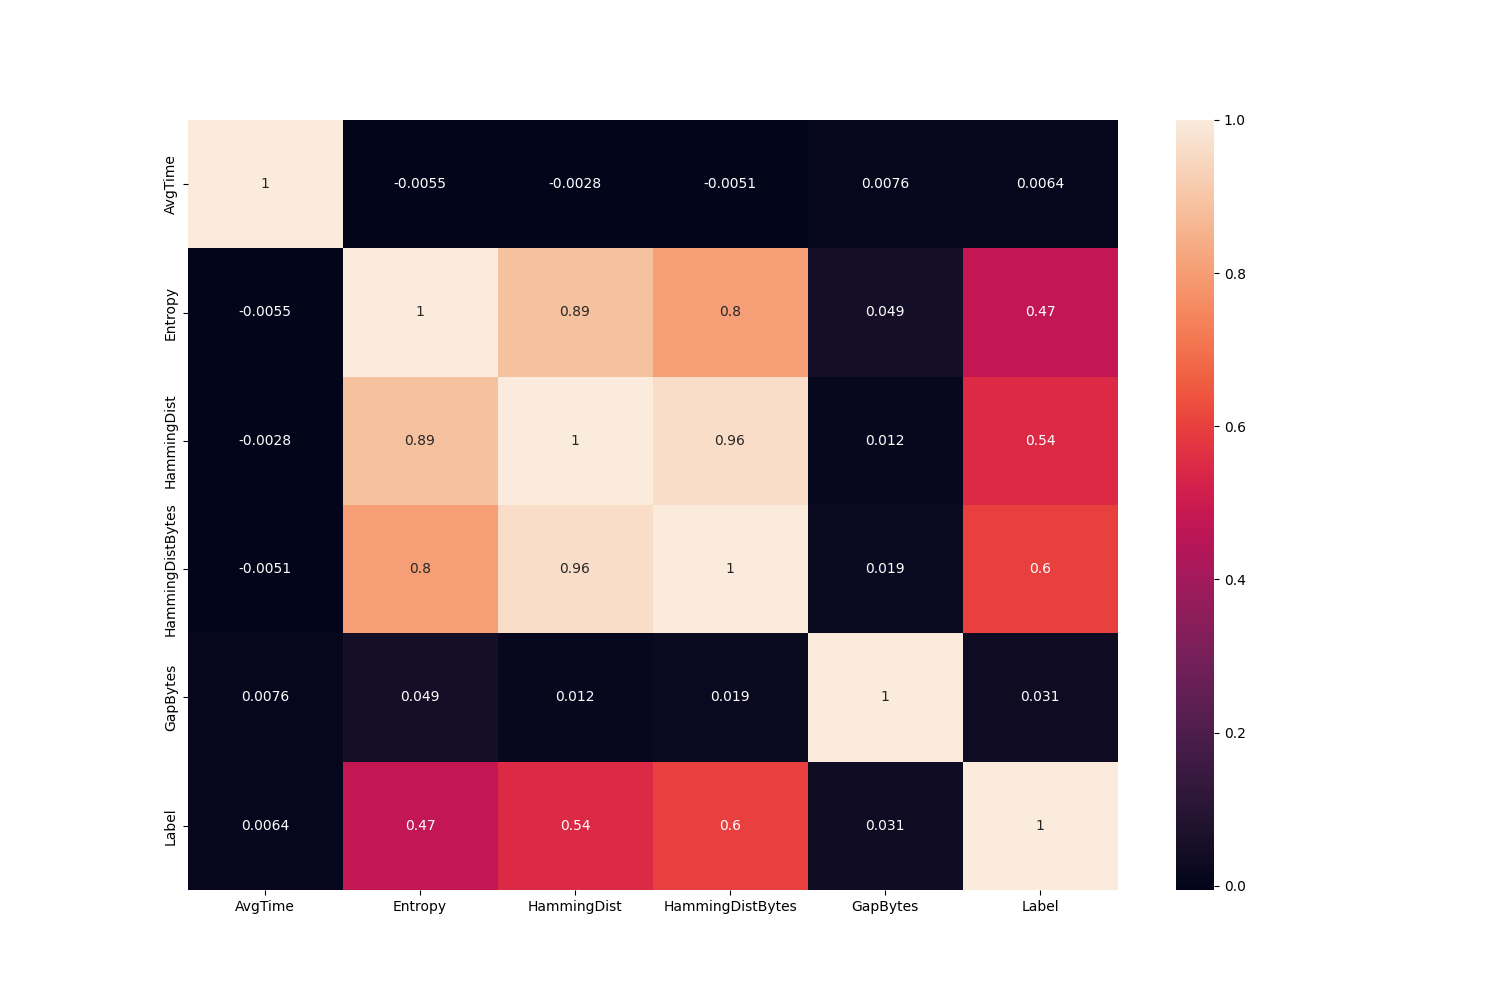
\includegraphics[width = \linewidth]{img/parts/app/feature_correlation/crysys/incr.png}
        \caption{CrySyS Lab - Adding an incrementing amount to packet payload}
        \label{subfig:fe_crysys_incr}
    \end{subfigure}
    
    \begin{subfigure}[b]{.6\linewidth}
        \centering
        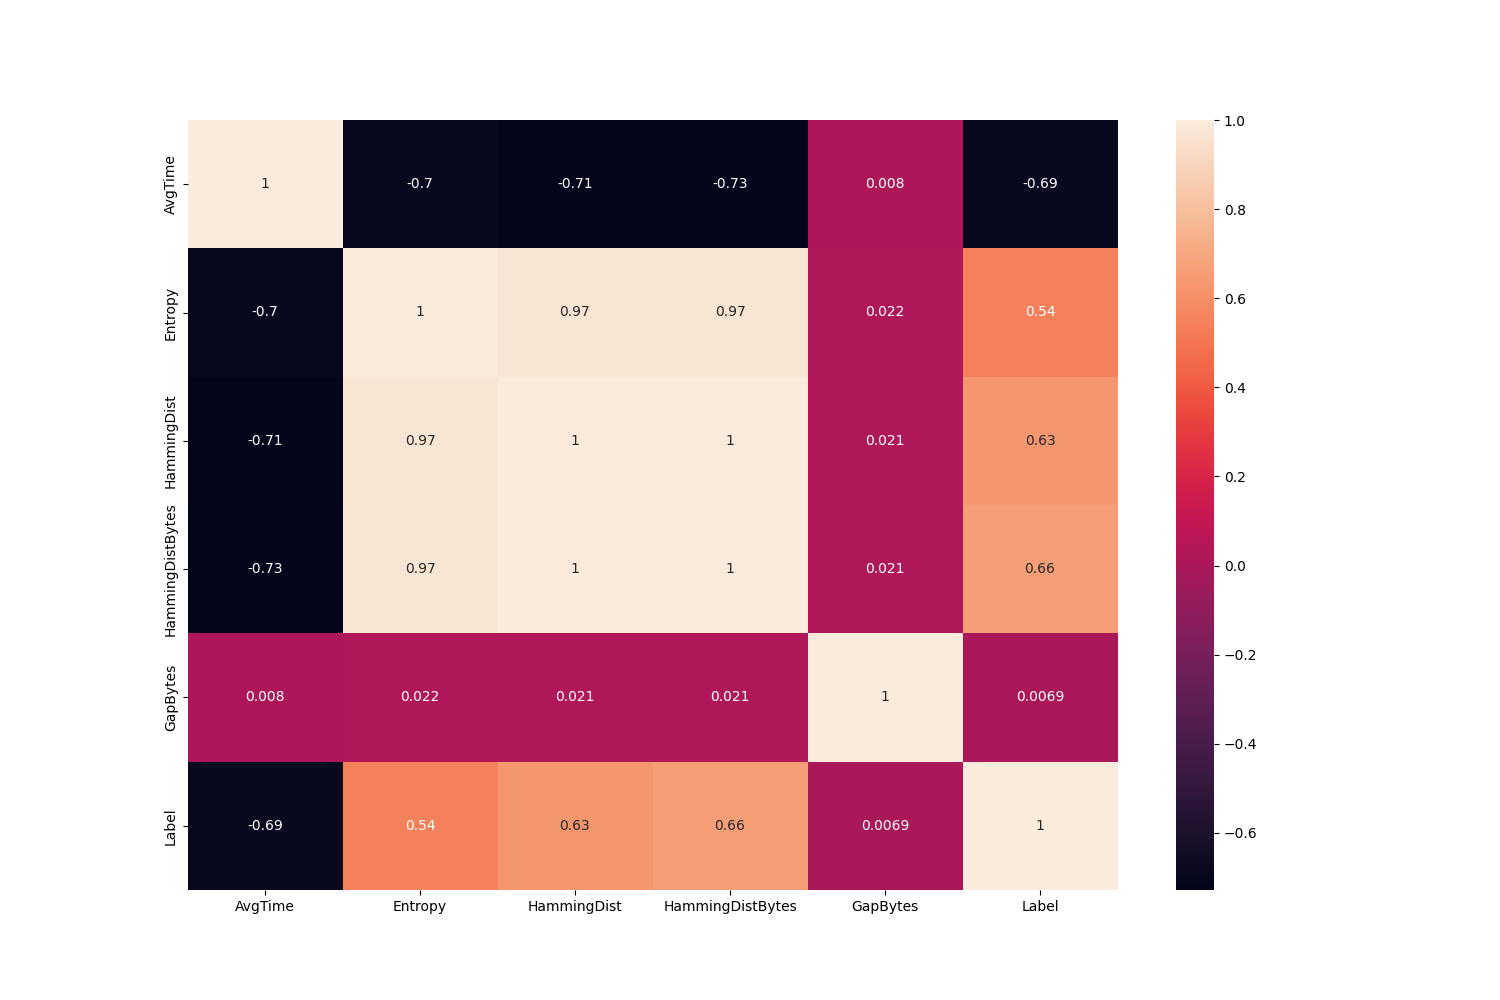
\includegraphics[width = \linewidth]{img/parts/app/feature_correlation/ieee_challenge/pre_submit_D.png}
        \caption{IEEE Car Hacking: Attack \& Defense Challenge 2020 - Attacks while driving}
        \label{subfig:fe_ieee_challende_d}
    \end{subfigure}
    
    \begin{subfigure}[b]{.6\linewidth}
        \centering
        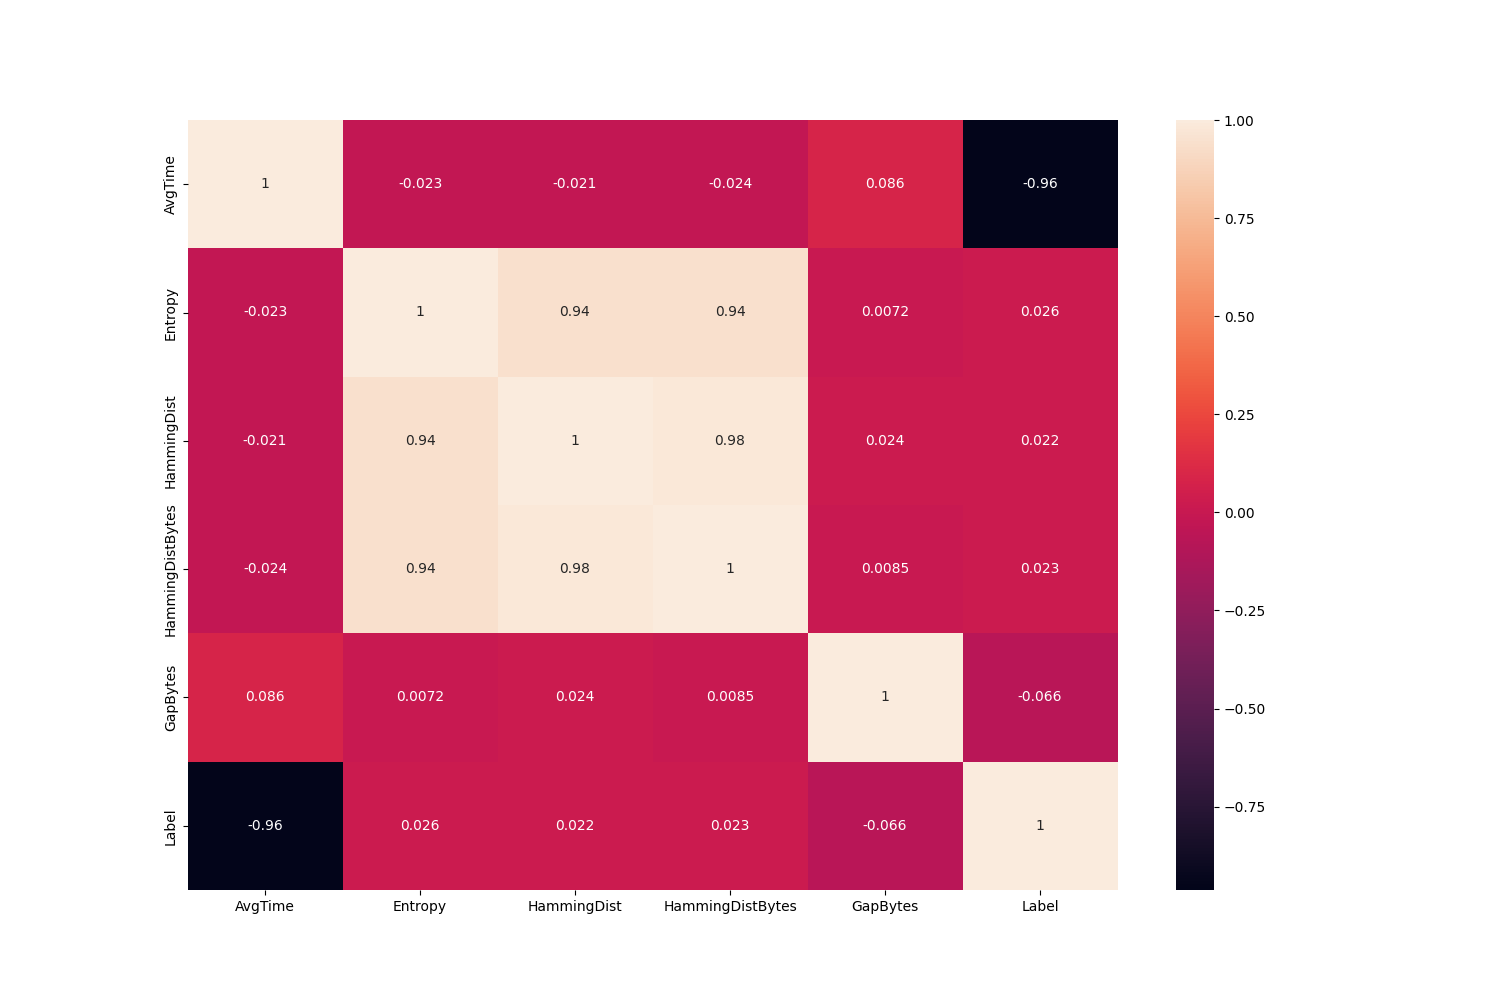
\includegraphics[width = \linewidth]{img/parts/app/feature_correlation/OpelAstra/replay.png}
        \caption{Automotive Controller Area Network (CAN) Bus Intrusion Dataset v2 - Replay attack}
        \label{subfig:fe_tue_opelastra}
    \end{subfigure}
    
    \caption{Correlation between extracted features}
    \label{fig:fe}
\end{figure}

Thus, after observing several attack types, including with and without packet insertion, the average byte-wise Hamming distance and the average arrival time between packets of the same ID appear to be the most promising in predicting whether an attack is present or not.

\section{Embedded system environment}
\label{sec:app_embedded}

To simulate the environment where the proposed system would be deployed, the program was written in Rust 1.62.0 and compiled to the ARM v7 architecture to run on a Raspberry Pi 4 Model B connected to the ECU cluster shown in Figure \ref{fig:setup}. Code documentation is available in Appendix \ref{apdx:sec:code_documentation}.\par

To verify if the system would be able to analyse real-time traffic, the number of packets per second it was able to process was recorded. This came at around 1600. However, it was unclear whether this was a bottleneck or if it was the real network throughput. To clear this, traffic was logged onto a \gls{csv} file and processed by the Raspberry Pi as if it was live traffic, but read from memory instead of a network socket. The average number of packets per second processed came at 39,195.426, while the average number of packets per second in the log file was 1,678.878. The proposed system should therefore be able to perform real-time analysis in an embedded environment. CPU usage was recorded as being 5\%, signalling that its implementation in a real ECU would not raise serious concerns about resource usage.\par
It is also important to assure that the algorithm does not consume too much power, as it would reduce the overall range of the vehicle. Figure \ref{fig:powerdraw} shows how much current the Raspberry Pi was drawing while executing the \gls{ids}. Applied voltage was constant at 4900mV. The baseline current was established to be at 400mA, and it rose up to 500mA when the \gls{ids} was executing. This comes at 0.5W, which is negligible.

\begin{figure}
    \centering
    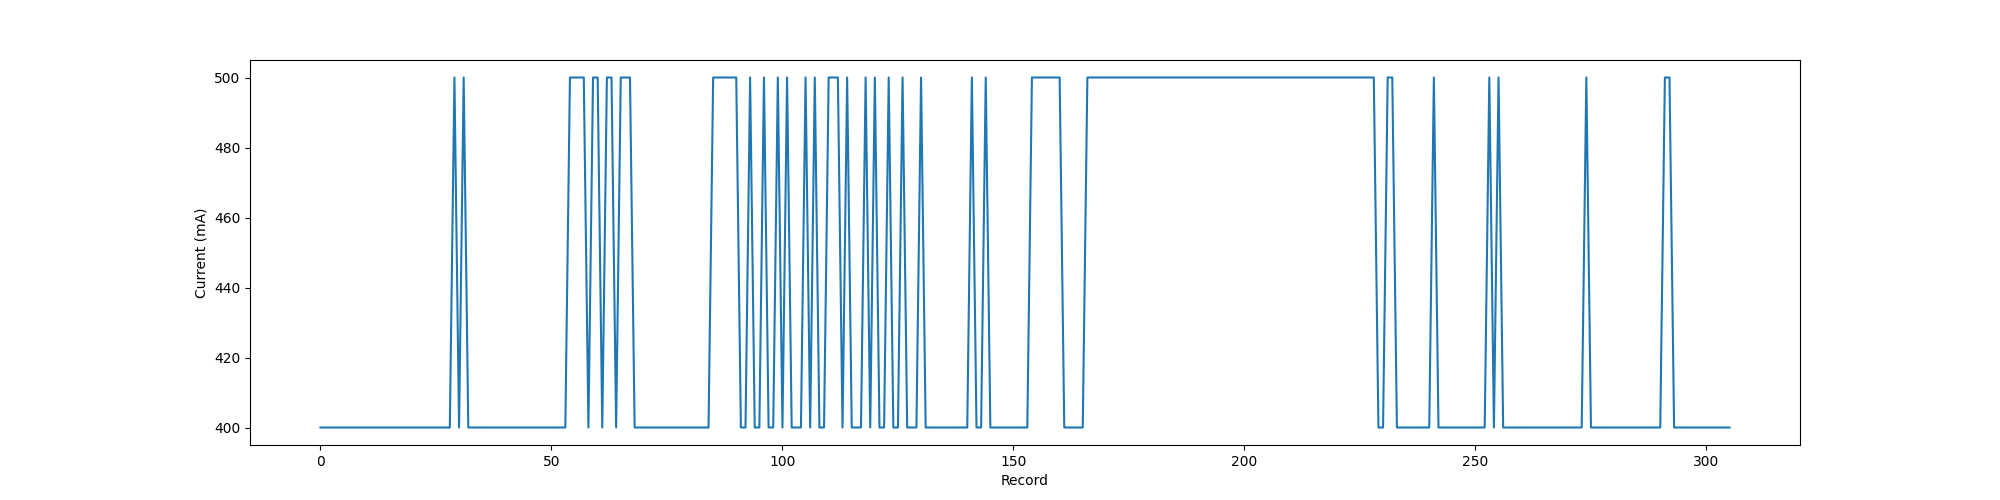
\includegraphics[width = \linewidth]{img/parts/app/powerdraw.png}
    \caption{Power consumption from the Raspberry Pi while executing the proposed \gls{ids}}
    \label{fig:powerdraw}
\end{figure}

\section{Execution}
\label{sec:app_exe}

A \gls{cli} was developed in order to facilitate application testing and deplyment. It consists of the following:

\begin{verbatim}
USAGE:
    aihds [OPTIONS]

OPTIONS:
        --extract-features <EXTRACT_FEATURES>
            Extracts features to CSV files
    -h, --help
            Print help information
        --live
            Run IDS in live mode
        --model <MODEL>
            Path to model to be loaded
        --monitor <LIST>
            IDs to monitor
        --streaming <URL>
            Run model in streaming mode
        --test <PATHS>
            Paths to the datasets required for testing the model,
            separated by ','
        --train <PATHS>
            Paths to the datasets required for training the model,
            separated by ','
    -V, --version
            Print version information
\end{verbatim}

Running the application in online mode is done with the \emph{live} option, while the \emph{training} option is used to indicate the file on which offline training will be performed. The \emph{streaming} option sends features and predictions as HTTP requests to the specified \gls{url}. An example of a graphical interface to visually represent the streaming data can be seen on Figure \ref{fig:website}.

\begin{figure}
    \centering
    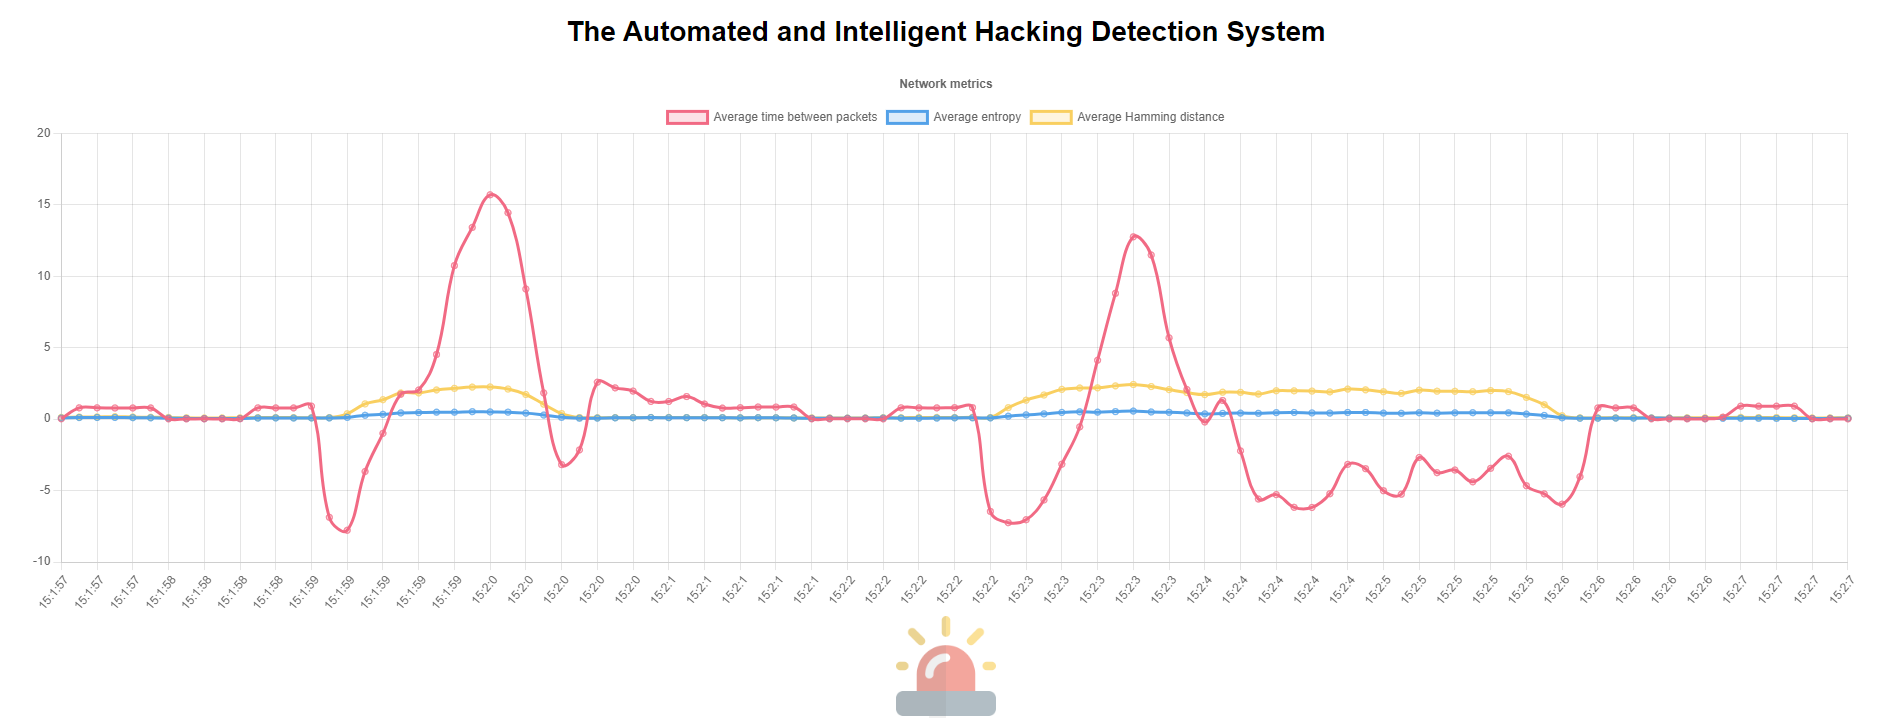
\includegraphics[width = \linewidth]{img/parts/app/website.png}
    \caption{Graphical interface}
    \label{fig:website}
\end{figure}
\chapter{Results}
\label{c:results}

Performance tests were performed in the datasets layed out in Chapter \ref{c:datasets}. These aim to show how the system performs in different environments and subject to a variety of attacks. Five metrics are used to evaluate system performance: False Negative (FN) rate, error rate, precision, recall, and F1-score (see \ref{subsec:performance_metrics}).\par
Values in bold were obtained when using three features as input to the model: average time between packets, entropy, and Hamming distance. The remaining values were obtained using only the average time between packets and Hamming distance.\par
Appendix \ref{apdx:sec:feature_extraction} contains illustrations of the system's performance over all the tests.

\section{Car Hacking Dataset}

Tests were made monitoring the IDs 350, 130, 131, 140, 2c2, 2b0, 316, 18f, 43f, and 440. The gear spoofing attack targets the ID 43f, and the RPM gauge spoofing attack targets the ID 316. Results are shown in Table \ref{tab:perf_car_hacking}.\par
When using only two features, the F1-score for both spoofing attacks are above 90\%. However, the occurrence of false positives remains high. Including entropy wields generally better results. Although the rate of false negatives is slightly worse, both precision and F1-score show bigger improvements. The fuzzing attack is harder to detect in both cases.\par
Graphics showing feature behaviour during tests can be seen of Figures \ref{fig:extract_carhacking_dos}, \ref{fig:extract_carhacking_fuzzy}, \ref{fig:extract_carhacking_gear}, and \ref{fig:extract_carhacking_rpm}.

\begin{table}
    \centering
    \begin{tabular}{*{6}{c}}
        \toprule
        \textbf{Data} & \textbf{FN rate} & \textbf{Error rate} & \textbf{Precision} & \textbf{Recall} & \textbf{F1-score}\\
        \midrule
        \multirow{2}{*}{Fuzzing} & 1.597\% & 20.300\% & 66.091\% & 98.403\% & 79.074\%\\
        & \textbf{1.632\%} & \textbf{10.746\%} & \textbf{79.134\%} & \textbf{98.368\%} & \textbf{87.709\%}\\
        \multirow{2}{*}{Gear spoofing} & 0.869\% & 10.470\% & 86.554\% & 99.131\% & 92.416\%\\
        & \textbf{1.062\%} & \textbf{2.910\%} & \textbf{96.698\%} & \textbf{98.938\%} & \textbf{97.799\%}\\
        \multirow{2}{*}{RPM spoofing} & 0.871\% & 10.256\% & 87.106\% & 99.129\% & 92.729\%\\
        & \textbf{0.948\%} & \textbf{2.723\%} & \textbf{96.891\%} & \textbf{99.052\%} & \textbf{98.034\%}\\
        \bottomrule
    \end{tabular}
    \caption{Performance metrics on Car Hacking dataset}
    \label{tab:perf_car_hacking}
\end{table}

\section{IEEE Car Hacking: Attack \& Defense Challenge 2020}

The model was trained by gathering a baseline from the attack-free datasets in the stationary and driving modes, separately. Twelve IDs were monitored in each state (44E, 164, 260, 140, 541, 386, 490, 366, 367, 563, 4CB, 50E for the stationary state and 44E, 164, 130, 140, 3A0, 386, 490, 366, 367, 563, 4CB, 2B0 for the driving state). To test the IDS' performance, the stationary model was executed on the datasets provided for the preliminary and final round of the competition, and the driving model was executed on the dataset provided for the preliminary round (the final round did not include a dataset for the driving state).\par
Test results are present in Table \ref{tab:perf_ieee_challenge}. Results for the stationary final and driving tests are above 90\% in both the precision and F1-score metrics. The IDS, however, did not perform so well in the stationary preliminary test. Adding entropy to the set of features reduces the amount of false positives, at the expense of a small increase in the amount of false negatives. The IDS performs slightly worse in the other two tests. Still, it may be preferable to use the three features.\par
Graphics showing feature behaviour during tests can be seen of Figures \ref{fig:extract_ieee_d}, \ref{fig:extract_ieee_s_s}, and \ref{fig:extract_ieee_s_f}.

\begin{table}
    \centering
    \begin{tabular}{*{6}{c}}
        \toprule
        \textbf{Data} & \textbf{FN rate} & \textbf{Error rate} & \textbf{Precision} & \textbf{Recall} & \textbf{F1-score}\\
        \midrule
        \multirow{2}{*}{Stationary Preliminary} & 0.601\% & 19.242\% & 71.264\% & 99.399\% & 83.013\%\\
        & \textbf{0.701\%} & \textbf{16.635\%} & \textbf{74.232\%} & \textbf{99.299\%} & \textbf{84.955\%}\\
        \multirow{2}{*}{Stationary Final} & 0.403\% & 4.478\% & 93.283\% & 99.597\% & 96.337\%\\
        & \textbf{0.403\%} & \textbf{8.004\%} & \textbf{88.349\%} & \textbf{99.597\%} & \textbf{93.636\%}\\
        \multirow{2}{*}{Driving} & 2.591\% & 1.218\% & 99.412\% & 97.409\% & 98.400\%\\
        & \textbf{3.935\%} & \textbf{2.140\%} & \textbf{98.427\%} & \textbf{96.065\%} & \textbf{97.184\%}\\
        \bottomrule
    \end{tabular}
    \caption{Performance metrics on the IEEE Car Hacking: Attack \& Defense Challenge 2020}
    \label{tab:perf_ieee_challenge}
\end{table}

\section{Automotive Controller Area Network (CAN) Bus Intrusion Dataset v2}

Here, the results the tests performed on the datasets described in \ref{subsec:tue_dataset} are shown in Table \ref{tab:perf_tue}. For both the dataset created from traffic gathered from an Opel Astra and a Renault Clio, the IDS was tested on payload fuzzing, message deletion, and replay attacks. For the Opel Astra, the monitored IDs were 0C9, 1C8, 1E2, 232, 348, 34A, 451, 0F1, 1F3, 1E5, and 1A1. For the Renault Clio, the monitored IDs were 2C6, 186, 18A, 1F6, 211, 217, 214, 218, 4FA, and 090. All monitored IDs include the IDs targeted in the attacks, with the rest chosen at random.\par
The payload fuzzing attack goes unnoticed. This happens because, in this case, the attack consists of the modification of the payload of 10 consecutive messages on a given ID, which does not affect either the entropy or Hamming distance values enough to trigger an alert.\par
Graphics showing feature behaviour during tests can be seen of Figures \ref{fig:extract_tue_opelastra_fuzzing}, \ref{fig:extract_tue_opelastra_deletion}, and \ref{fig:extract_tue_opelastra_replay}.

\begin{table}
    \centering
    \begin{tabular}{*{6}{c}}
        \toprule
        \multicolumn{6}{c}{\textbf{Opel Astra}}\\
        \textbf{Data} & \textbf{FN rate} & \textbf{Error rate} & \textbf{Precision} & \textbf{Recall} & \textbf{F1-score}\\
        \midrule
        \multirow{2}{*}{Payload fuzzing} & 100.000\% & 0.408\% & N/A & 0.000\% & N/A\\
        & \textbf{100.000\%} & \textbf{0.408\%} &  \textbf{N/A} & \textbf{0.000\%} & \textbf{N/A}\\
        \multirow{2}{*}{Message deletion} & 18.750\% & 0.491\% & 100.000\% & 81.250\% & 89.655\%\\
        & \textbf{18.750\%} & \textbf{0.491\%} & \textbf{100.000\%} & \textbf{81.250\%} & \textbf{89.655\%}\\
        \multirow{2}{*}{Replay} & 0.000\% & 0.000\% & 100.000\% & 100.000\% & 100.000\%\\
        & \textbf{0.000\%} & \textbf{0.000\%} & \textbf{100.000\%} & \textbf{100.000\%} & \textbf{100.000\%}\\
        \bottomrule
        \toprule
        \multicolumn{6}{c}{\textbf{Renault Clio}}\\
        \textbf{Data} & \textbf{FN rate} & \textbf{Error rate} & \textbf{Precision} & \textbf{Recall} & \textbf{F1-score}\\
        \midrule
        \multirow{2}{*}{Payload fuzzing} & 100.000\% & 2.800\% & 0.000\% & 0.000\% & N/A\\
        & \textbf{100.000\%} & \textbf{2.800\%} & \textbf{0.000\%} & \textbf{0.000\%} & \textbf{N/A}\\
        \multirow{2}{*}{Message deletion} & 27.273\% & 3.629\% & 100.000\% & 72.727\% & 84.746\%\\
        & \textbf{27.273\%} & \textbf{3.629\%} & \textbf{100.000\%} & \textbf{72.727\%} & \textbf{84.211\%}\\
        \multirow{2}{*}{Replay} & 0.000\% & 0.000\% & 100.000\% & 100.000\% & 100.000\%\\
        & \textbf{0.000\%} & \textbf{0.000\%} & \textbf{100.000\%} & \textbf{100.000\%} & \textbf{100.000\%}\\
        \bottomrule
    \end{tabular}
    \caption{Performance metrics on the Automotive Controller Area Network (CAN) Bus Intrusion Dataset v2}
    \label{tab:perf_tue}
\end{table}

\section{CrySyS Lab}

Table \ref{tab:perf_crysys} shows the results of the tests performed on the CrySyS Lab dataset and the generated modification attacks, as described in \ref{sec:dataset_crysys}. Tests were made monitoring 10 IDs (110, 120, 140, 180, 1A0, 280, 290, 295, 300, and 301) and only the attacked ID (120).

\begin{table}
    \centering
    \begin{tabular}{*{6}{c}}
        \toprule 
        \multicolumn{6}{c}{\textbf{Monitoring 10 IDs}}\\
        \midrule
        \textbf{Attack} & \textbf{FN rate} & \textbf{Error rate} & \textbf{Precision} & \textbf{Recall} & \textbf{F1-score}\\
        \midrule
        \multirow{2}{*}{Constant value} & 100.000\% & 40.451\% & 0.000\% & 0.000\% & N/A\\
        & \textbf{100.000\%} & \textbf{40.451\%} & \textbf{0.000\%} & \textbf{0.000\%} & \textbf{N/A}\\
        \multirow{2}{*}{Random value} & 8.992\% & 3.687\% & 99.851\% & 91.008\% & 95.225\%\\
        & \textbf{8.311\%} & \textbf{3.357\%} & \textbf{100.000\%} & \textbf{91.689\%} & \textbf{95.665\%}\\
        \multirow{2}{*}{Adding an increasing value} & 94.959\% & 38.415\% & 97.368\% & 5.051\% & 9.585\%\\
        & \textbf{96.185\%} & \textbf{38.855\%} & \textbf{100.000\%} & \textbf{3.815\%} & \textbf{7.349\%}\\
        \multirow{2}{*}{Decreasing value} & 100.000\% & 40.396\% & N/A & 0.000\% & N/A\\
        & \textbf{100.000\%} & \textbf{40.396\%} & \textbf{N/A} & \textbf{0.000\%} & \textbf{N/A}\\
        \multirow{2}{*}{Delta of 1000} & 99.728\% & 40.341\% & 66.667\% & 0.272\% & 0.543\%\\
        & \textbf{99.864\%} & \textbf{40.341\%} & \textbf{100.000\%} & \textbf{0.136\%} & \textbf{0.272\%}\\
        \bottomrule
        \toprule
        \multicolumn{6}{c}{\textbf{Monitoring 1 ID}}\\
        \midrule
        \textbf{Attack} & \textbf{FN rate} & \textbf{Error rate} & \textbf{Precision} & \textbf{Recall} & \textbf{F1-score}\\
        \midrule
        \multirow{2}{*}{Constant value} & 4.511\% & 1.911\% & 100.000\% & 95.489\% & 97.692\\
        & \textbf{5.263\%} & \textbf{2.229\%} & \textbf{100.000\%} & \textbf{94.737\%} & \textbf{97.297}\\
        \multirow{2}{*}{Random value} & 1.504\% & 0.637\% & 100.000\% & 98.496\% & 99.242\%\\
        & \textbf{0.752\%} & \textbf{0.318\%} & \textbf{100.000\%} & \textbf{99.248\%} & \textbf{99.623\%}\\
        \multirow{2}{*}{Adding an increasing value} & 38.346\% & 16.242\% & 100.000\% & 61.654\% & 76.279\%\\
        & \textbf{24.812\%} & \textbf{10.510\%} & \textbf{100.000\%} & \textbf{75.188\%} & \textbf{85.837\%}\\
        \multirow{2}{*}{Decreasing value} & 100.000\% & 42.357\% & N/A & 0.000\% & N/A\\
        & \textbf{100.000\%} & \textbf{42.357\%} & \textbf{N/A} & \textbf{0.000\%} & \textbf{N/A}\\
        \multirow{2}{*}{Delta of 1000} & 100.000\% & 42.357\% & N/A & 0.000\% & N/A\\
        & \textbf{100.000\%} & \textbf{42.357\%} & \textbf{N/A} & \textbf{0.000\%} & \textbf{N/A}\\
        \bottomrule
    \end{tabular}
    \caption{Performance metrics on the CrySyS Lab datasets}
    \label{tab:perf_crysys}
\end{table}

\section{CES}

The \gls{ids} was trained with the attack-free dataset monitoring the IDs A0, A1, AB, CA, DE, F1, F3, F9, FA, 145, 231, 29D, and 510. Since this dataset is unlabelled, performance metrics, like precision, cannot be used. Instead, Figures \ref{fig:ces_fuzzy} and \ref{fig:ces_spoofing} shows how feature values behave during the fuzzing and spoofing attacks, respectively.\par
In the case of the fuzzing attack, since packets were inserted at a rather slow rate (200ms), the average time between packets, shown in Figure \ref{subfig:ces_fuzzy_avgtime}, does not behave abnormally. Network entropy also remained largely unchanged (Figure \ref{subfig:ces_fuzzy_entropy}). In Figure \ref{subfig:ces_fuzzy_hammingdist}, which shows Hamming distance values, two identifiable spikes corresponding to the two instances of the attack can be seen.\par
As for the spoofing attack, analysis of packet frequency (Figure \ref{subfig:ces_spoofing_avgtime}) does not show any anomalies given the slow rate at which the packets were inserted. Entropy, which can be seen in Figure \ref{subfig:ces_spoofing_entropy}, was also not altered. Hamming distance, however, became anomalous during the two instances of the attack represented by the spikes in Figure \ref{subfig:ces_spoofing_hammingdist}.

\begin{figure}
    \centering
    \begin{subfigure}[b]{.6\linewidth}
        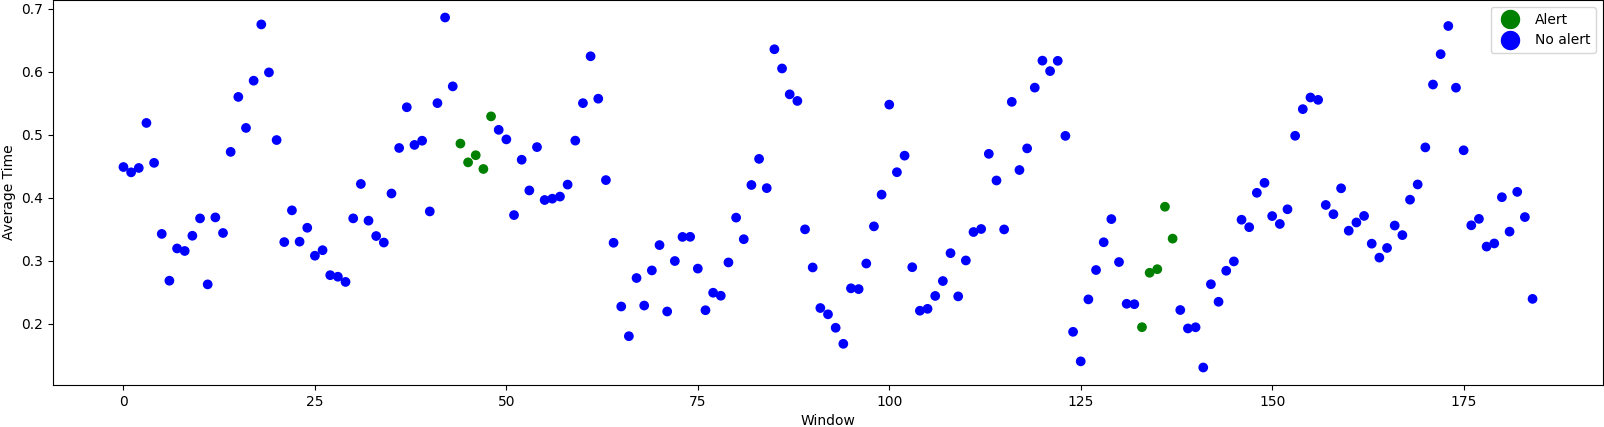
\includegraphics[width = \linewidth]{img/parts/app/tests/ces/fuzzy/AvgTime.png}
        \caption{Average time between packets}
        \label{subfig:ces_fuzzy_avgtime}
    \end{subfigure}
    \begin{subfigure}[b]{.6\linewidth}
        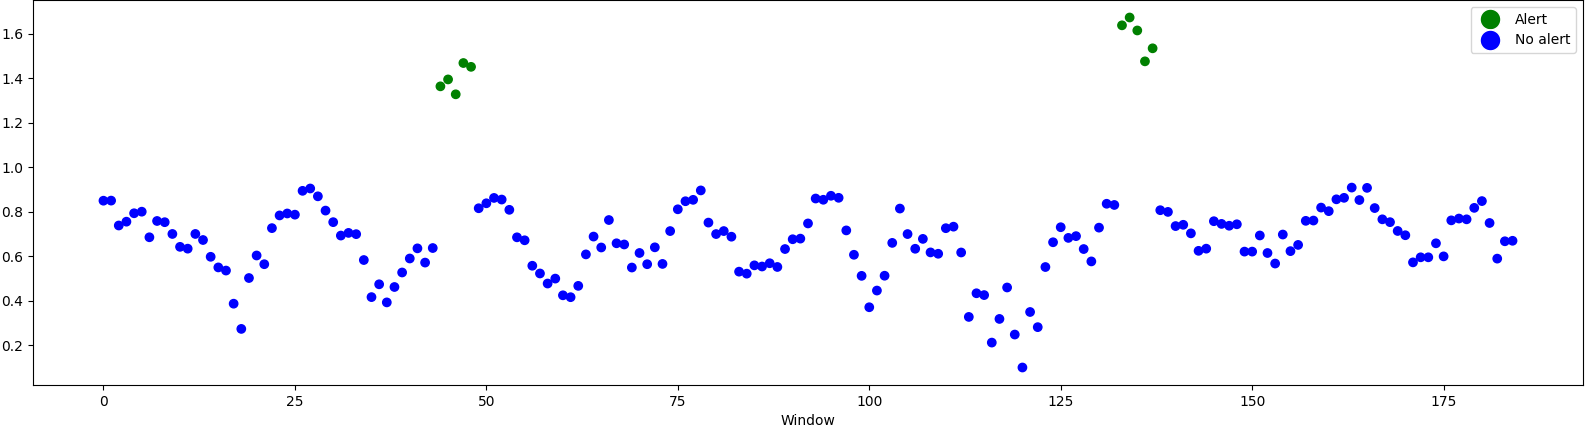
\includegraphics[width = \linewidth]{img/parts/app/tests/ces/fuzzy/HammingDist.png}
        \caption{Hamming distance}
        \label{subfig:ces_fuzzy_hammingdist}
    \end{subfigure}
    \begin{subfigure}[b]{.6\linewidth}
        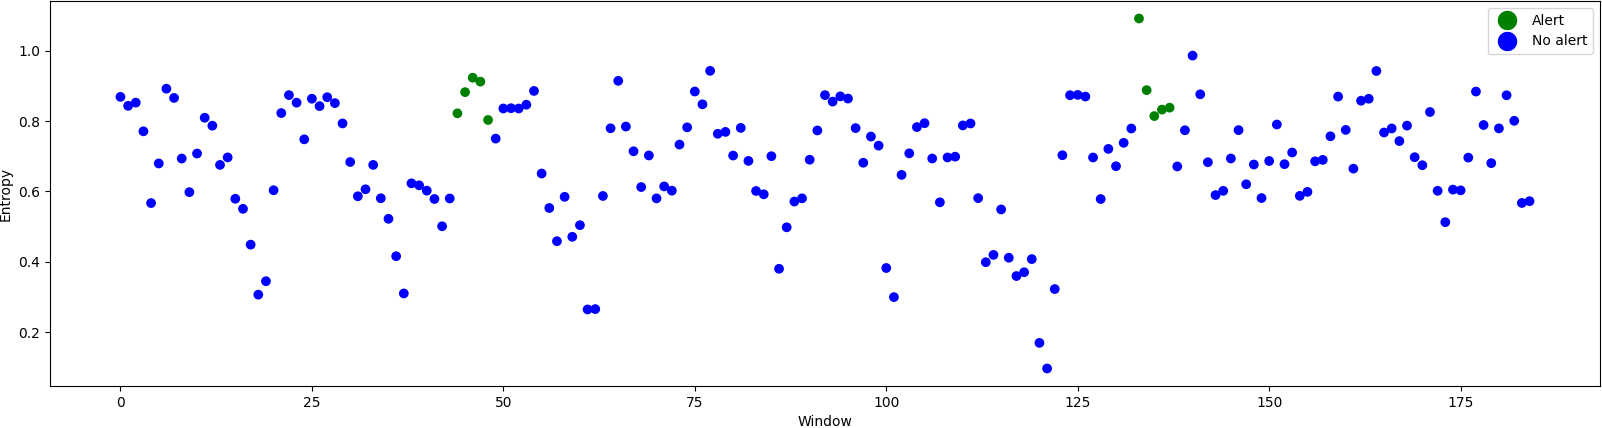
\includegraphics[width = \linewidth]{img/parts/app/tests/ces/fuzzy/Entropy.png}
        \caption{Entropy}
        \label{subfig:ces_fuzzy_entropy}
    \end{subfigure}
    \caption{Features extracted from the fuzzing attack present in the CES dataset}
    \label{fig:ces_fuzzy}
\end{figure}

\begin{figure}
    \centering
    \begin{subfigure}[b]{.6\linewidth}
        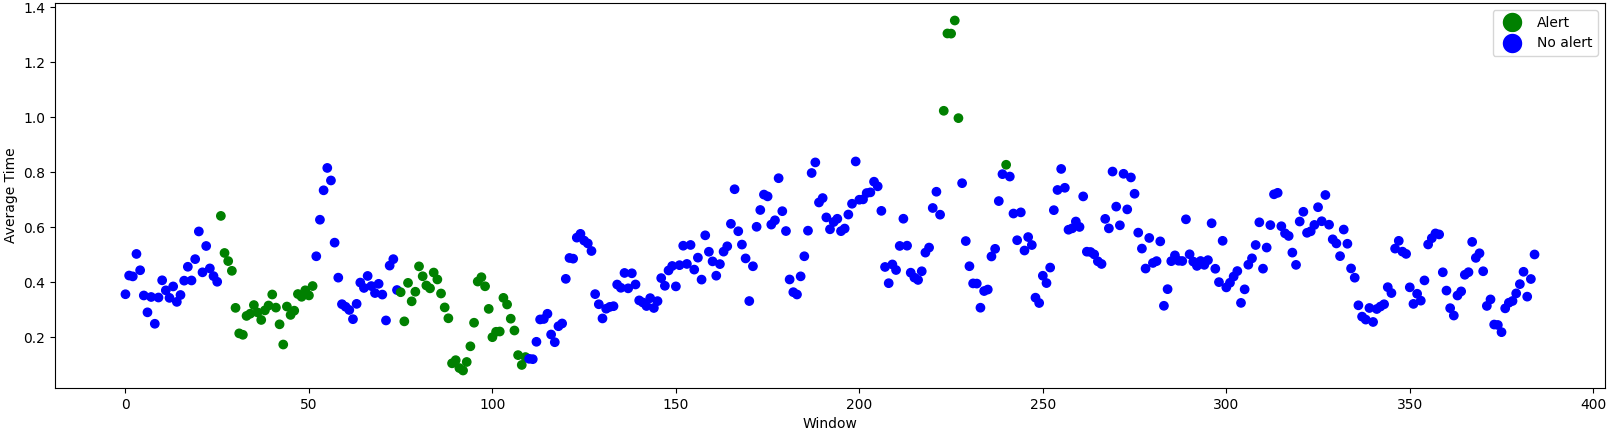
\includegraphics[width = \linewidth]{img/parts/app/tests/ces/spoofing/AvgTime.png}
        \caption{Average time between packets}
        \label{subfig:ces_spoofing_avgtime}
    \end{subfigure}
    \begin{subfigure}[b]{.6\linewidth}
        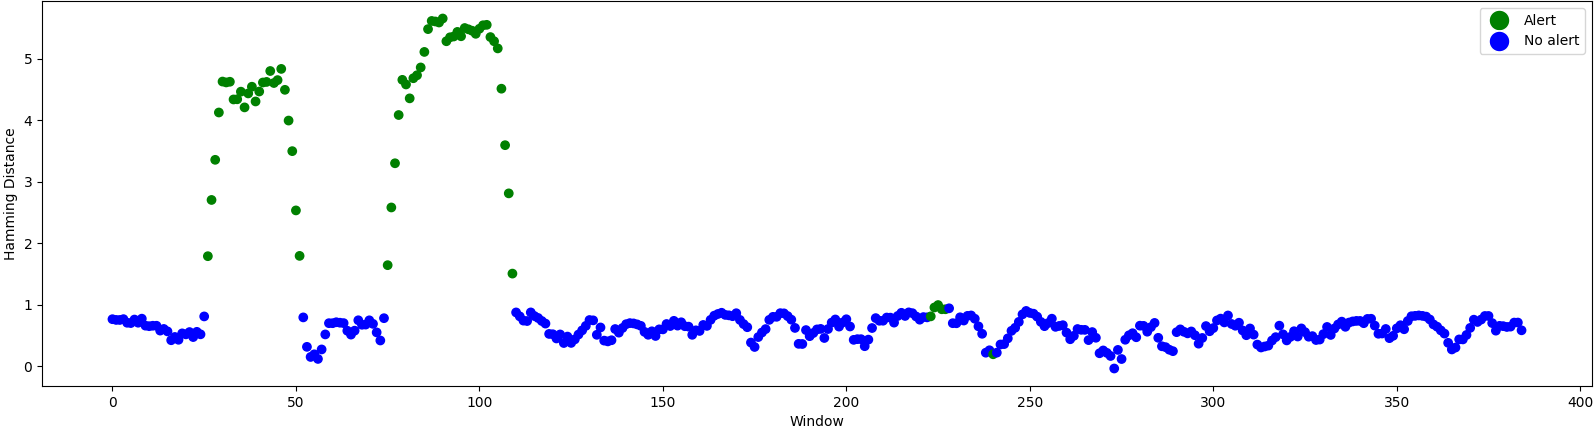
\includegraphics[width = \linewidth]{img/parts/app/tests/ces/spoofing/HammingDist.png}
        \caption{Hamming distance}
        \label{subfig:ces_spoofing_hammingdist}
    \end{subfigure}
    \begin{subfigure}[b]{.6\linewidth}
        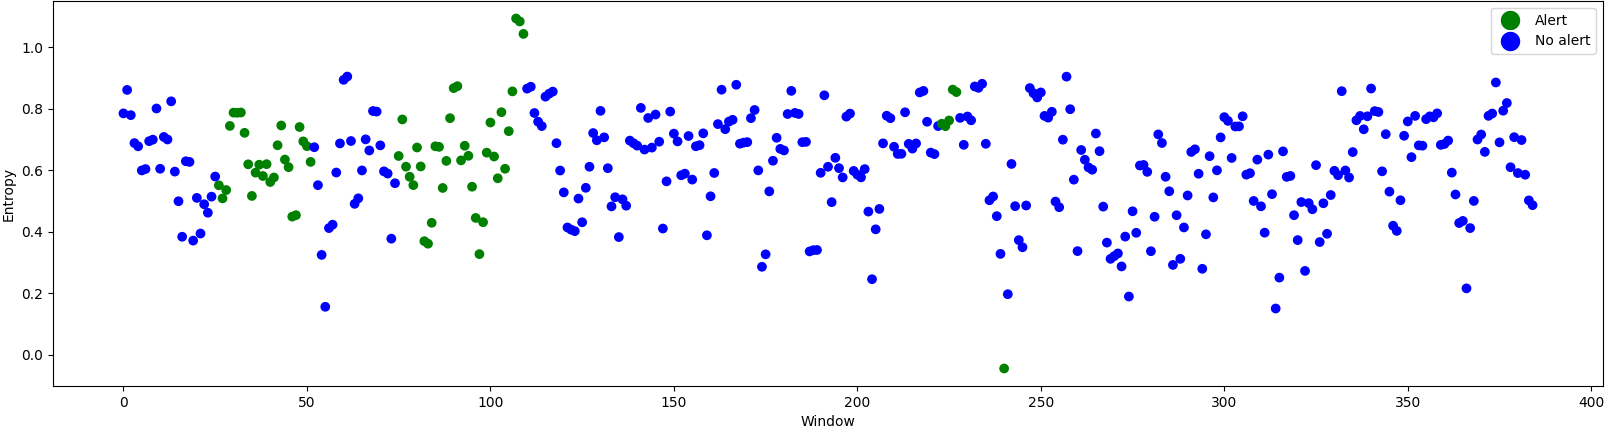
\includegraphics[width = \linewidth]{img/parts/app/tests/ces/spoofing/Entropy.png}
        \caption{Entropy}
        \label{subfig:ces_spoofing_entropy}
    \end{subfigure}
    \caption{Features extracted from the spoofing attack present in the CES dataset}
    \label{fig:ces_spoofing}
\end{figure}

\part{Conclusion}
\chapter{Future work}
\chapter{Conclusion}
\label{c:conclusion}

\section{Limitations and Future Work}

Because of the lightweight nature of the proposed solution, it could become overloaded if the number of messages being analysed is too high. Currently, this is alleviated by monitoring only a subset of IDs per application instance. However, as automotive applications become more complex, and as network throughput increases, scalability issues may arise. Alternatives such as different network metrics to monitor may be investigated as a potential solution, as well as a possible replacement to the method of averaging the features concerning different IDs to obtain a single value.\par

Another limitation in detecting an anomaly relies in the fact that attacks that span only some messages go largely undetected. This is because the deviation from normal behaviour caused by such a small number of anomalous messages is not enough to cause a significant alteration in the features of the window being analysed.\par

Traditionally, the training phase of machine learning includes some kind of hyperparameter tuning. However, there is no hyperparameter tuning for the \gls{ocsvm} here implemented, with the hyperparameter values being hard-coded. This is because traditional tuning algorithms rely on validation and testing datasets to evaluate model performance, but this would not apply to a real-world scenario where the model is trained only with attack-free data. The inclusion of such a process in the training phase would likely increase performance.

\section{Summary}

Continuous automotive development has brought forth a new concept of the vehicle. Modern vehicles are capable of running many complex applications, as well as communicating with each other and with road infrastructure. This allows the vehicle to aid the driver through \gls{adas} applications such as lane-assist and adaptive cruise control, as well as gather traffic information and other aspects of its surroundings. Vehicles capable of fully autonomous driving are also in active development.\par

The ability to connect to the exterior significantly raised the risk of attacks compared to when vehicles were self-contained. This new vector of attack motivated a new search for security solutions in the automotive space. One such solution is based on the concept of the \gls{ids}, which has existed in traditional networks for many years. An \gls{ids} analyses network traffic and signals when an attack is ocurring.\par

This dissertation presented an implementation of this concept for the \acrlong{can} using machine learning to perform blind traffic analysis. It uses a combination of packet timing and information-theory algorithms to detect attacks, meaning that it does not need to understand packet syntax. This is relevant because packet syntax is not standardised and is highly proprietary, meaning that the application can therefore be implemented by a variety of manufacturers in a plug-and-play fashion.\par

Although the solution is not without its limitations, it builds upon previous research by combining both packet frequency and information-theoretic metrics into a single machine learning model capable of being executed in real-time in a resource-constrained environment.\par

To make modern vehicles secure, a variety of solutions must come together. This includes \glspl{tpm}, network encryption, and many others. This application is yet another component contributing to achieving this ever-important goal.
%\chapter{Next steps}

%\textcolor{blue}{The scope of our project is relatively large. Because of this, we decided to divide the development into two main phases. The first we called the offline phase. The main goal during this step is to develop a model capable of signalling anomalous traffic in existing data sets. Using existing data sets will jump-start our development and allow quick iterations over different possibilities we want to explore. The second one is called the online phase. The main objective will be to test and validate the model found previously in a physical environment,i.e., connected to an existing vehicle ECU cluster. The detailed steps for both phases are listed below.}\par

Project development is split in two main phases: offline and online. The main goal of the offline phase is to develop a model capable of signalling anomalous traffic in existing data sets. Using these data sets will jump-start our development and allow quick iterations over different possibilities we want to explore. For the online phase, the main objective is to test and validate the model in a real environment, \textit{i.e.}, connected to an existing vehicle ECU cluster. The detailed steps for both phases are listed below.\par

The offline phase can be split into the following steps:
\begin{itemize}
    \item \textbf{Data set gathering}, where existing CAN data sets containing attacks are inspected and saved.
    \item \textbf{Exploration of possible models}, in which various machine learning approaches are investigated and attempted.
    \item \textbf{Analysis and choice of a model}, where a choice is made on the machine learning best approach to the problem.
    \item \textbf{Development of the IDS prototype}, where the proposed solution is implemented in code.
\end{itemize}

And the online phase is composed of these tasks:
\begin{itemize}
    \item \textbf{Definition of the test attacks}, in which various CAN attack procedures are investigated and a choice is made as to what will be attempted. 
    \item \textbf{Gathering of live data}, where data from a real vehicle cluster is gathered while attempting the chosen attacks.
    \item \textbf{Real-time testing of the model}, where the developed IDS is used to detect the attacks.
\end{itemize}

%\textcolor{blue}{We plan to write the final document in parallel with the development phase. This approach will ensure we do not forget any important details and findings. At the end of the project, there is still some buffer time reserved to conclude and improve the document.}\par

The writing of the final document is to be done in parallel with the development phase. This approach will ensure we do not forget any important details and findings. At the end of the project, there is still some buffer time reserved to conclude and improve the document. Figure \ref{fig:timeline} shows a Gantt chart with detailing the proposed timeline. Steps in blue are part of the offline phase of development, while the steps in green are part of the online phase. Orange signals the project's wrapping.

%\begin{itemize}
%    % ----- OFFLINE -----
%    \item Recolha de datasets                        - 7/02
%    \item Exploração dos vários modelos possíveis    - 31/03
%    \item Análise e escolha de o melhor modelo       - 15/05
%    % ----- ONLINE -----
%    \item Definição dos ataques de teste             - 31/05
%    \item Recolha de dados "reais"                   - 15/06
%    \item Teste do modelo em real time               - 15/07
%    
%    \item Finalizar documento                        - 31/07
%\end{itemize}

\begin{figure}
    \centering
    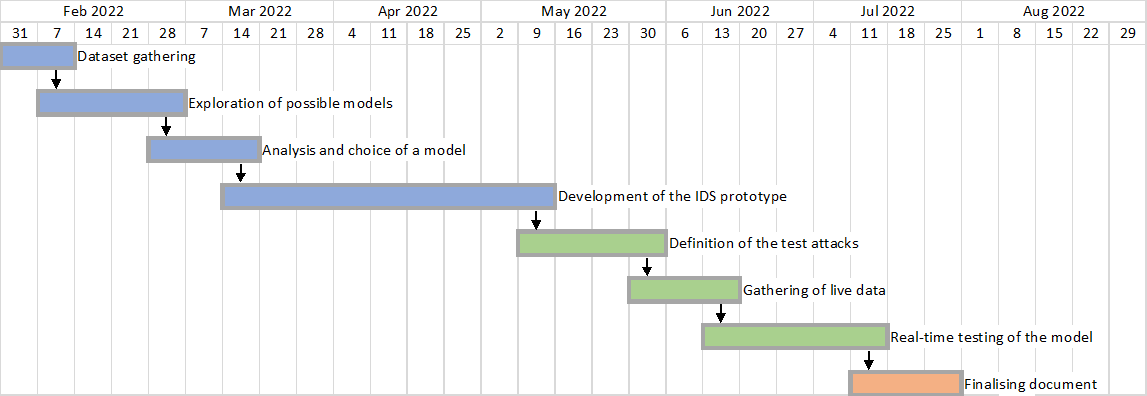
\includegraphics[width = \textwidth]{img/parts/conclusion/timeline.png}
    \caption{Project timeline (blue for the offline phase, green for the online phase, and orange for conclusion)}
    \label{fig:timeline}
\end{figure}
		
\bookmarksetup{startatroot}
\addtocontents{toc}{\bigskip}
\cleardoublepage

\bibliography{library}

\printglossary[type=\acronymtype]

\appendix
\renewcommand\chaptername{Appendix}

\chapter{Feature selection}
\label{apdx:sec:feature_selection}
\chapter{Feature selection}
\label{apdx:sec:feature_selection}

Here, the collection of graphs generated as part of the feature selection process is presented.

\begin{figure}
    \centering
    
    \begin{subfigure}[b]{.6\linewidth}
        \centering
        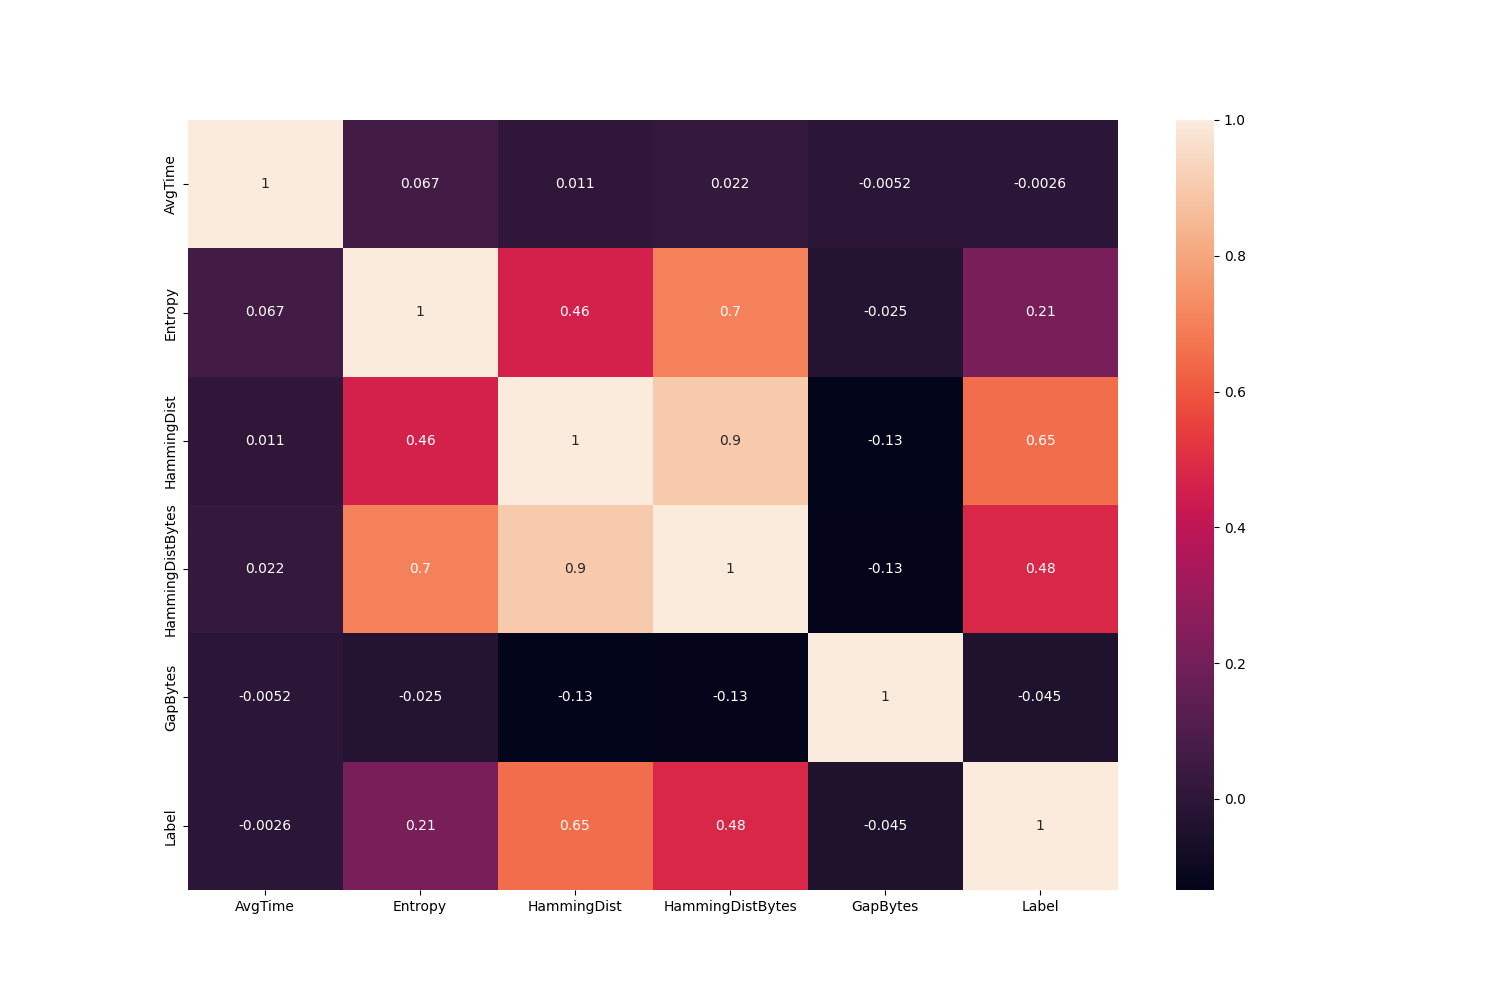
\includegraphics[width = \linewidth]{img/parts/app/feature_correlation/car_hacking/fuzzy.png}
        \caption{Fuzzing attack}
        \label{subfig:apdx_fe_car_hacking_fuzzy}
    \end{subfigure}
    
    \begin{subfigure}[b]{.6\linewidth}
        \centering
        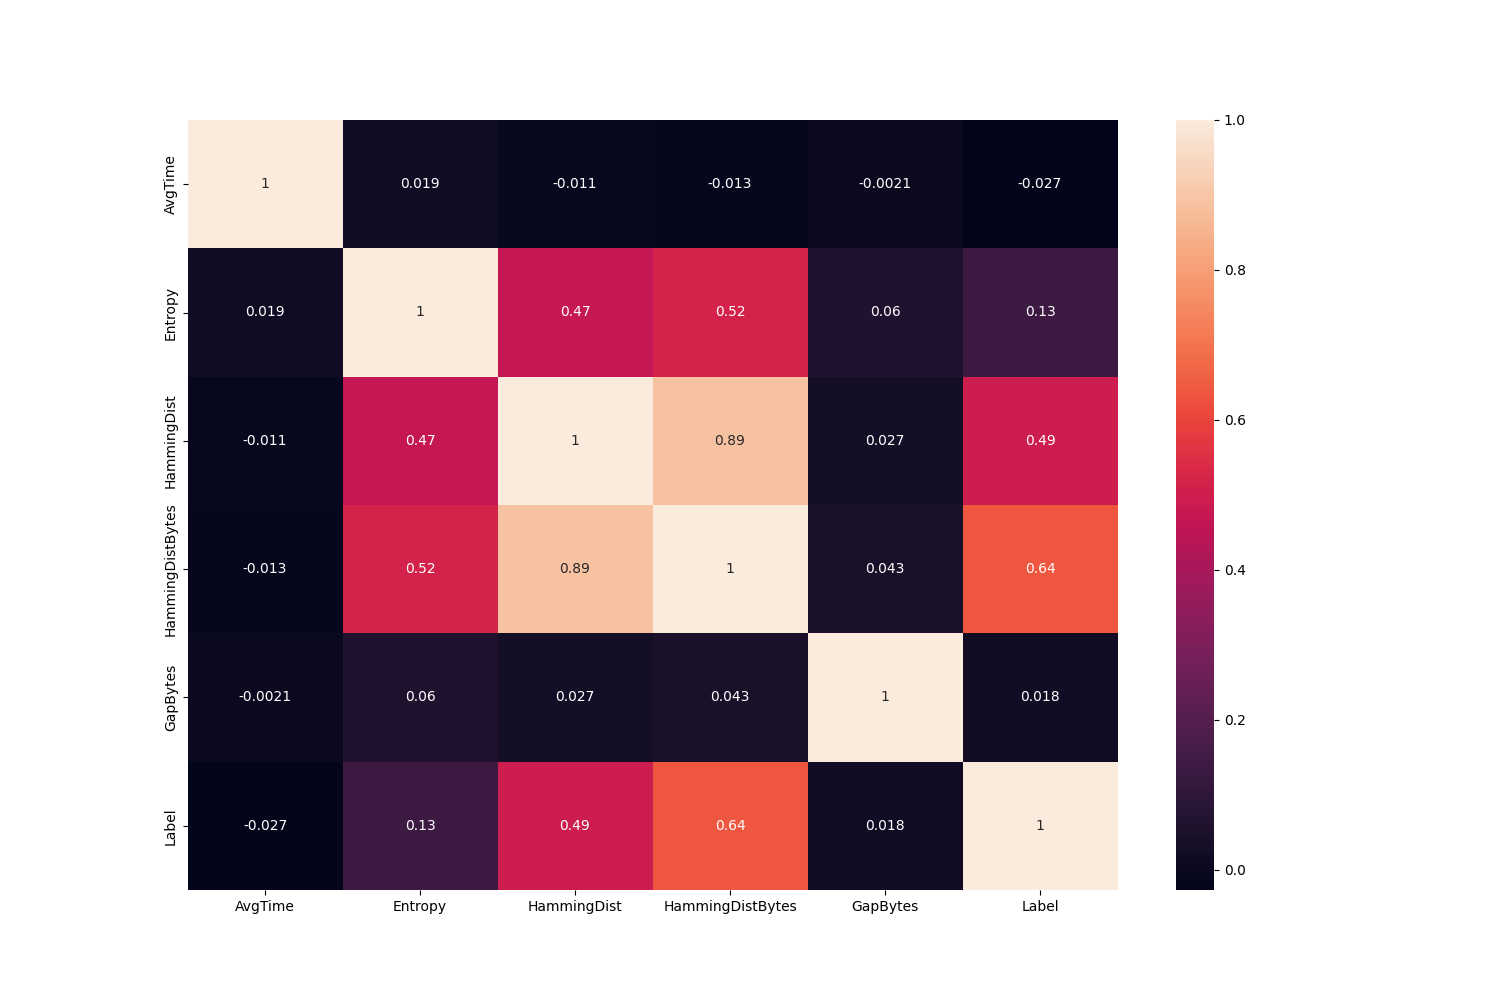
\includegraphics[width = \linewidth]{img/parts/app/feature_correlation/car_hacking/gear.png}
        \caption{Gear spoofing attack}
        \label{subfig:apdx_fe_car_hacking_gear}
    \end{subfigure}
    
    \begin{subfigure}[b]{.6\linewidth}
        \centering
        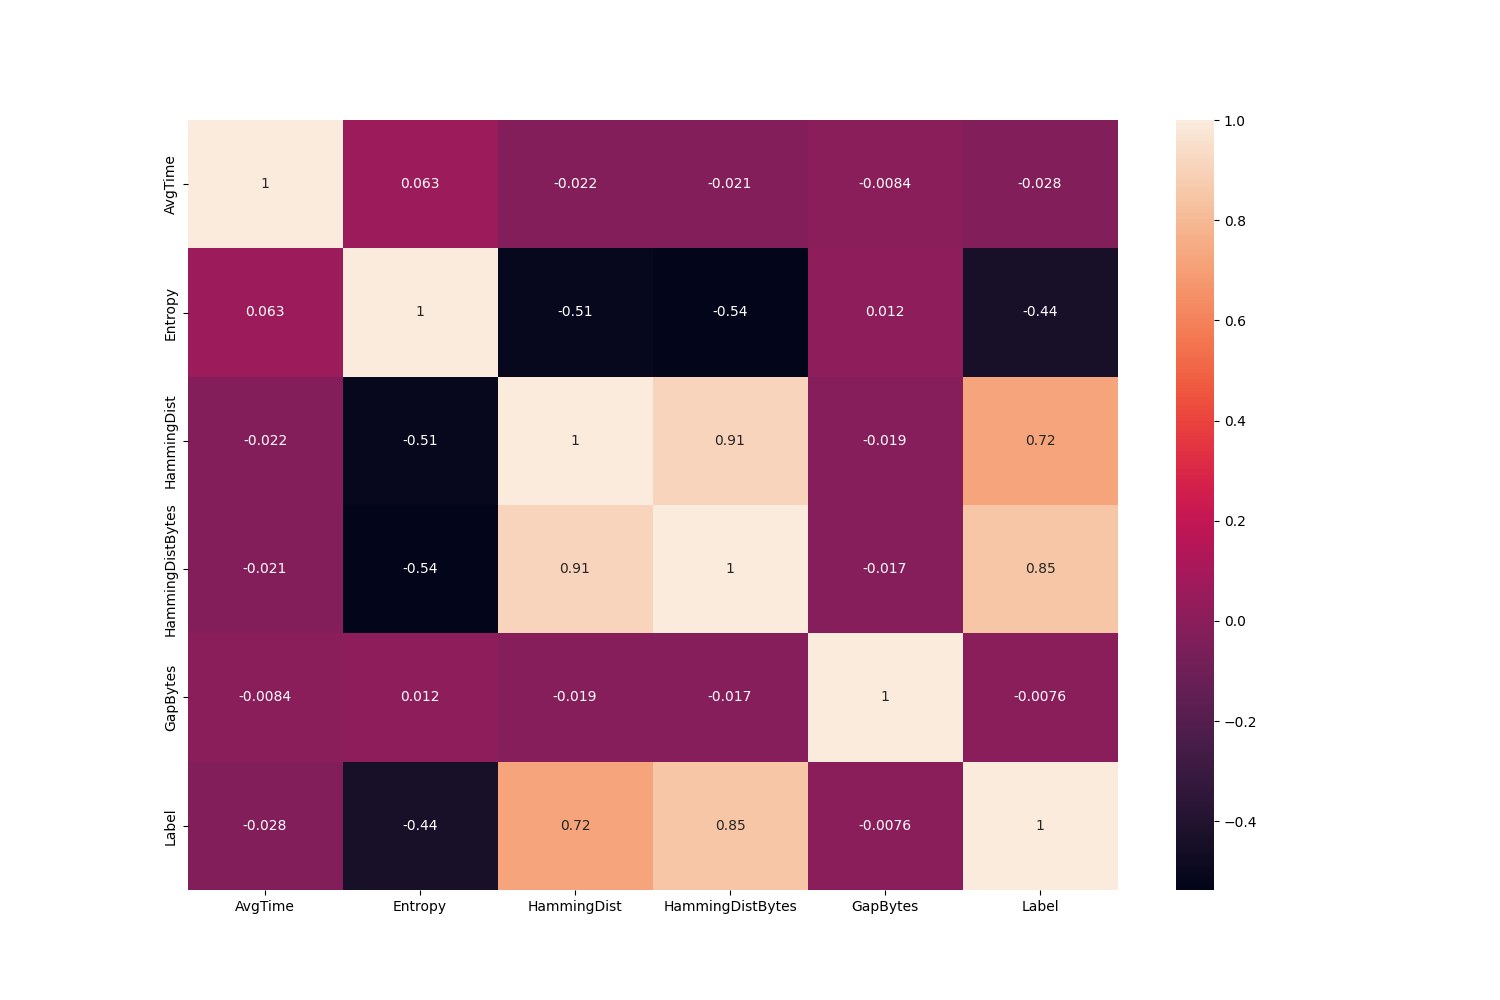
\includegraphics[width = \linewidth]{img/parts/app/feature_correlation/car_hacking/rpm.png}
        \caption{RPM spoofing attack}
        \label{subfig:apdx_fe_car_hacking_rpm}
    \end{subfigure}
    
    \caption{Correlation between extracted features obtained from the Car Hacking dataset}
    \label{fig:apdx_fe_car_hacking}
\end{figure}

\begin{figure}
    \centering
    
    \begin{subfigure}[b]{.6\linewidth}
        \centering
        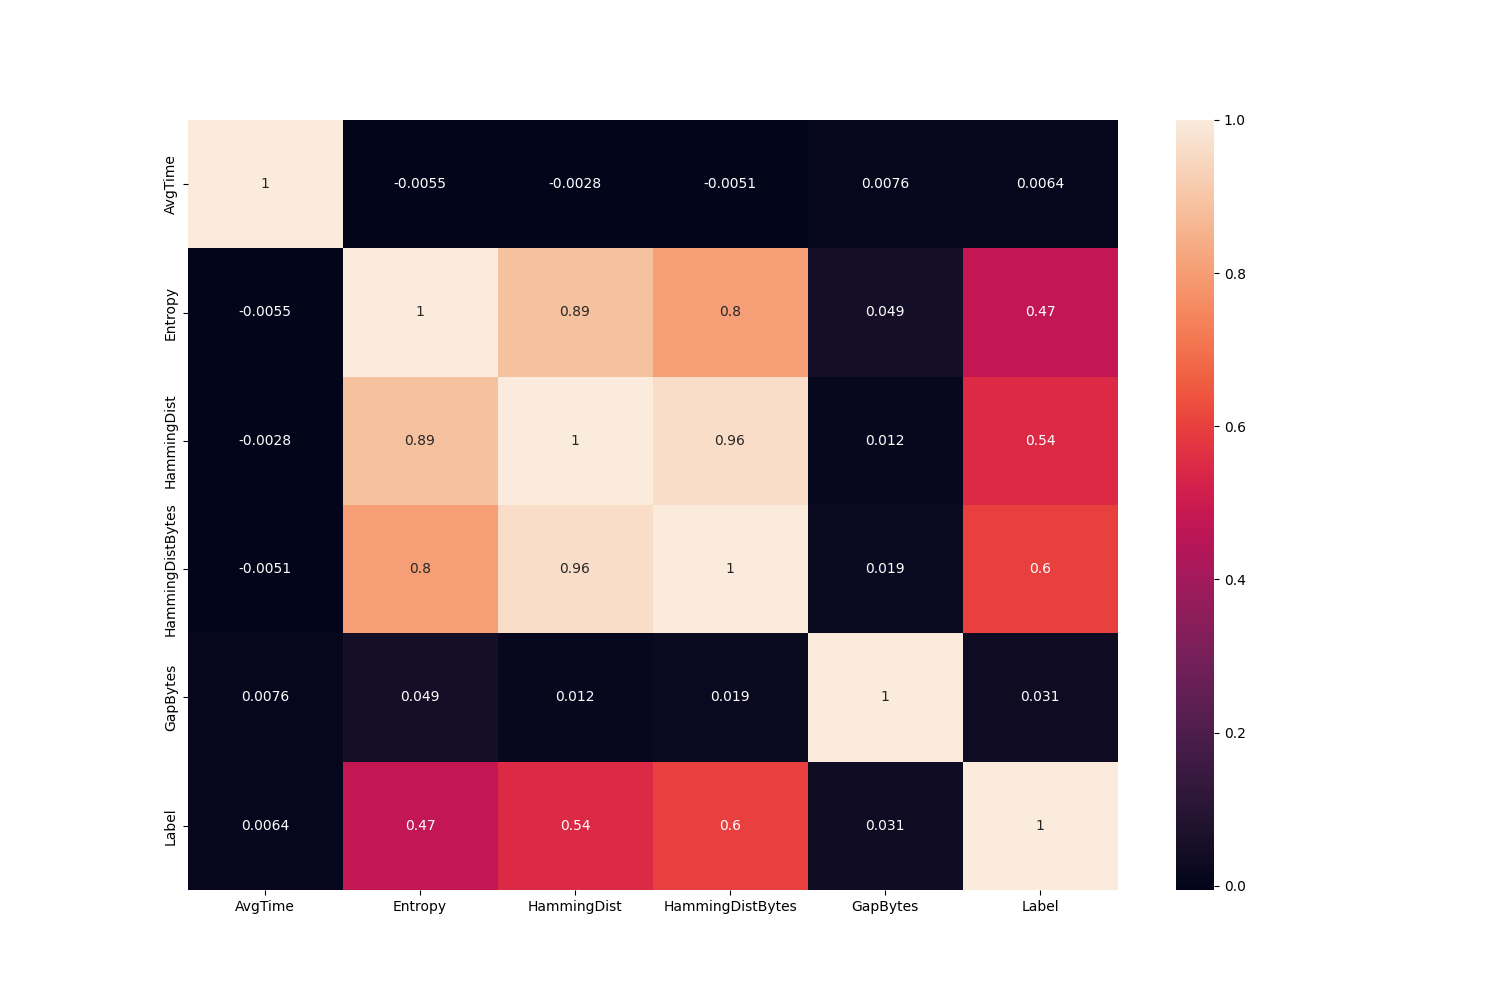
\includegraphics[width = \linewidth]{img/parts/app/feature_correlation/crysys/incr.png}
        \caption{Incremental payload modification attack}
        \label{subfig:apdx_fe_crysys_incr}
    \end{subfigure}
    
    \begin{subfigure}[b]{.6\linewidth}
        \centering
        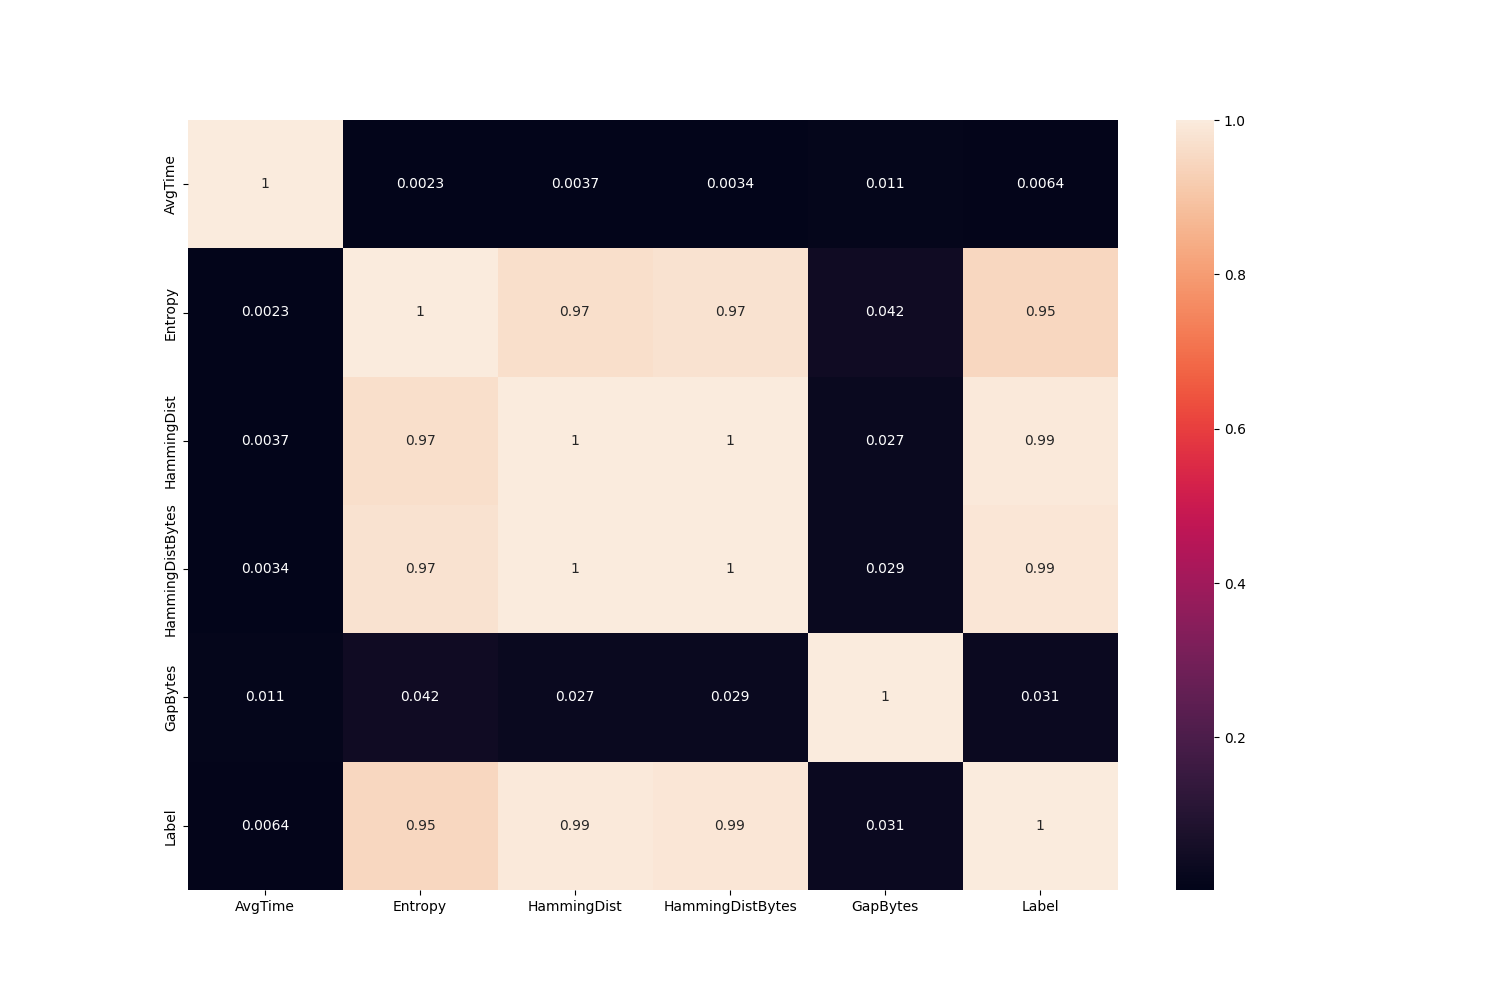
\includegraphics[width = \linewidth]{img/parts/app/feature_correlation/crysys/random.png}
        \caption{Random payload modification attack}
        \label{subfig:apdx_fe_crysys_random}
    \end{subfigure}
    
    \caption{Correlation between extracted features obtained from the CrySyS Lab dataset}
    \label{fig:apdx_fe_crysys}
\end{figure}

\begin{figure}
    \centering
    
    \begin{subfigure}[b]{.6\linewidth}
        \centering
        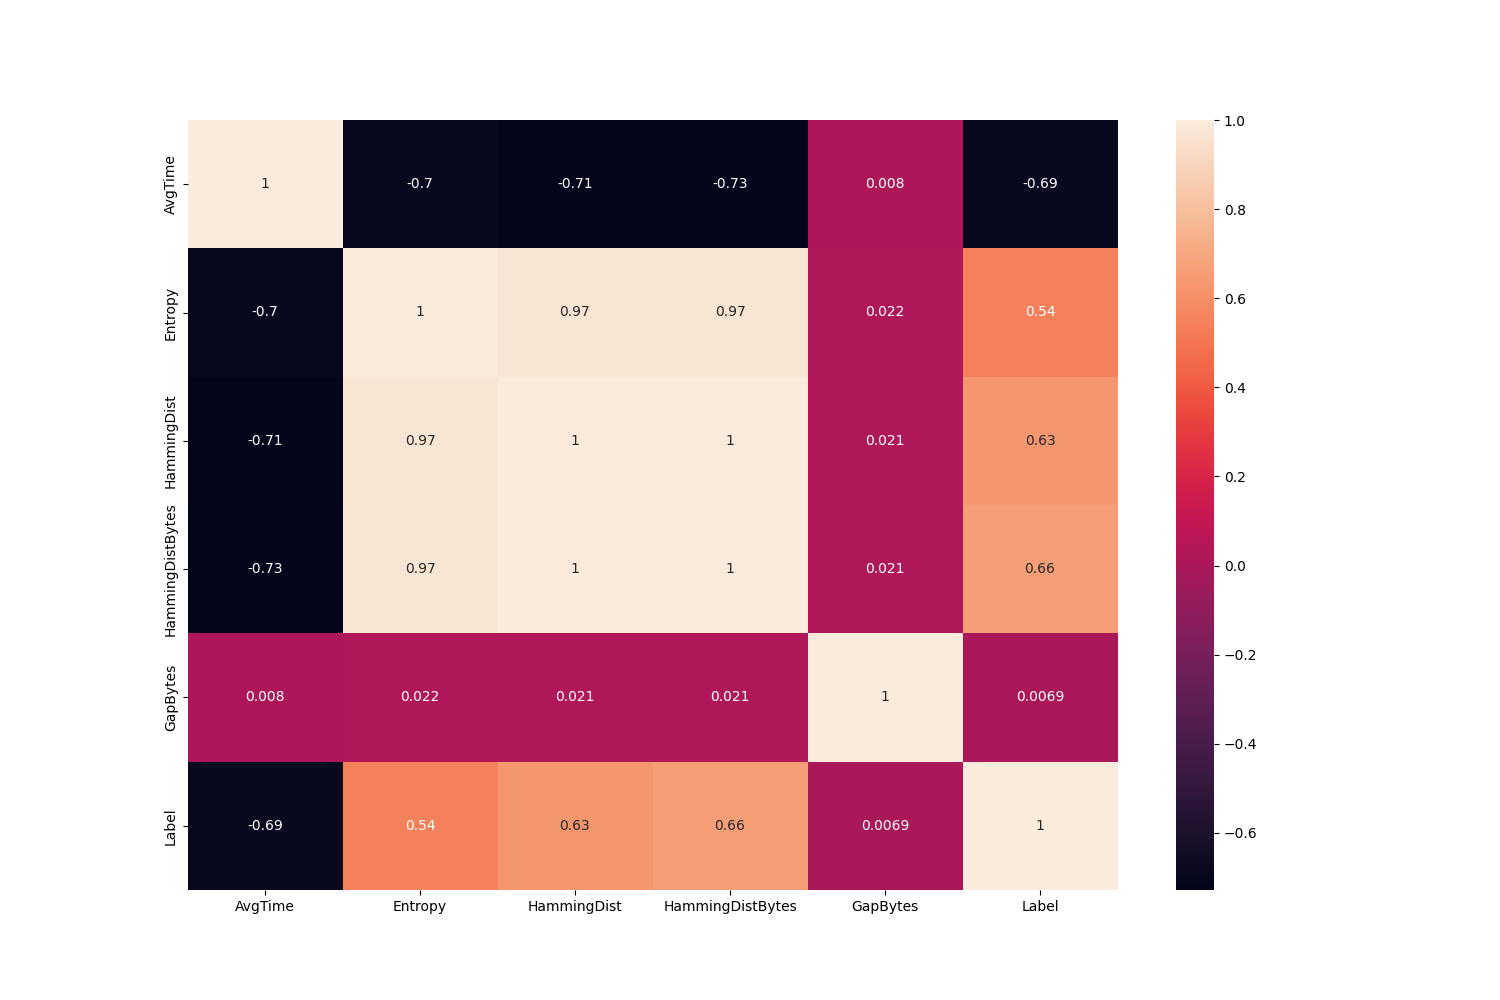
\includegraphics[width = \linewidth]{img/parts/app/feature_correlation/ieee_challenge/pre_submit_D.png}
        \caption{Attacks while driving}
        \label{subfig:apdx_fe_ieee_d}
    \end{subfigure}
    
    \begin{subfigure}[b]{.6\linewidth}
        \centering
        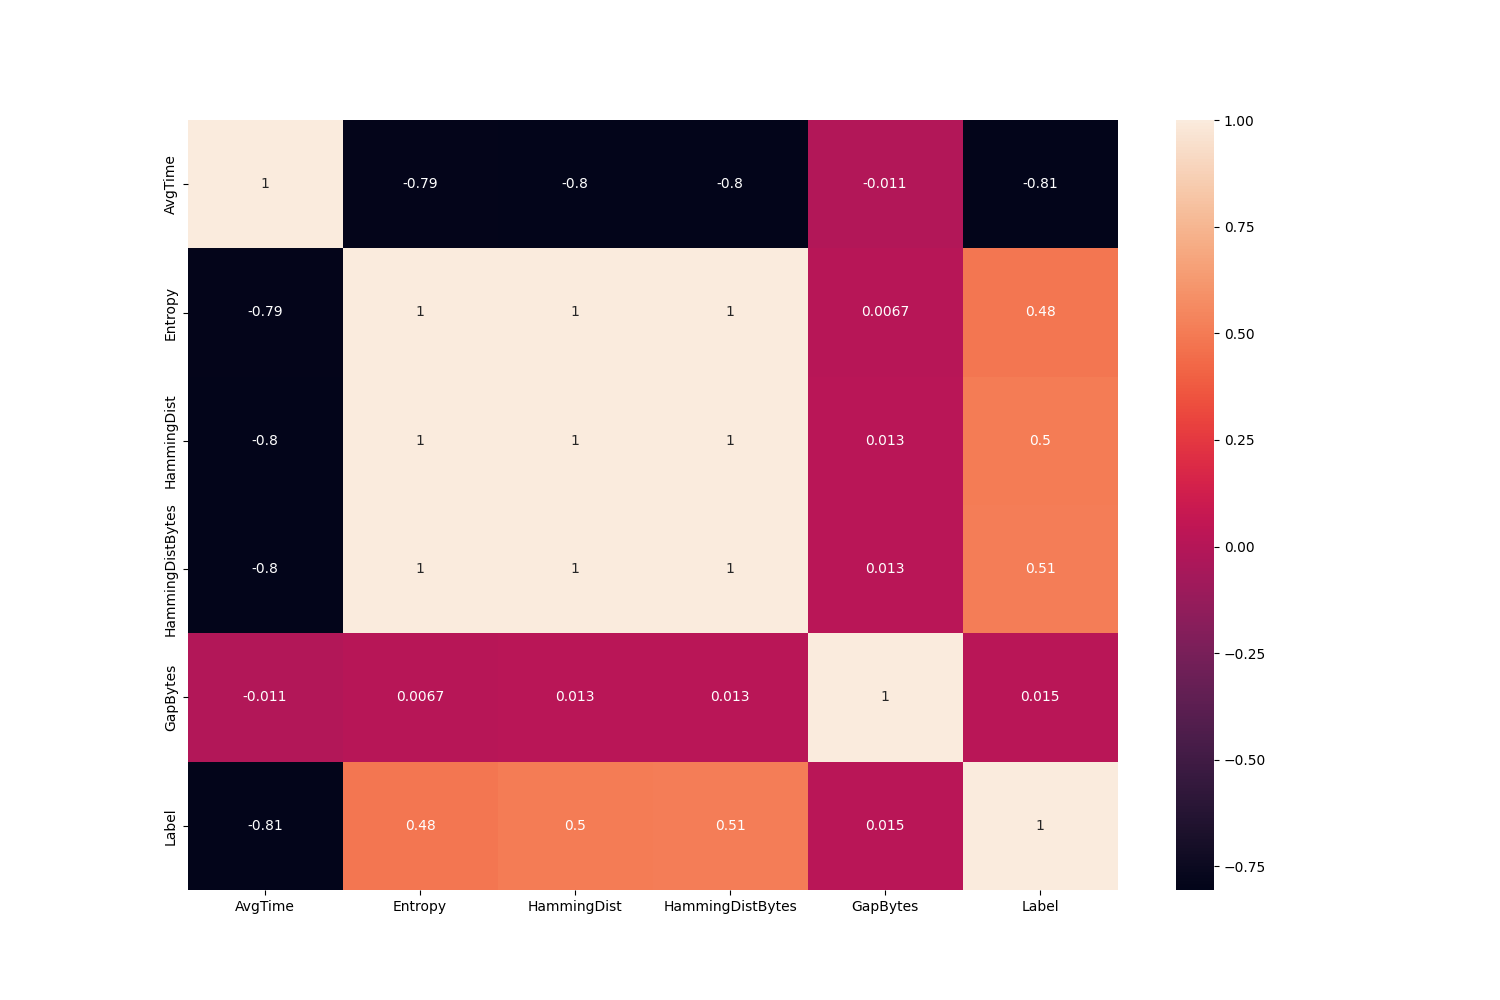
\includegraphics[width = \linewidth]{img/parts/app/feature_correlation/ieee_challenge/pre_submit_S.png}
        \caption{Attacks while stationary}
        \label{subfig:apdx_fe_ieee_s}
    \end{subfigure}
    
    \caption{Correlation between extracted features obtained from the IEEE Car Hacking: Attack \& Defense Challenge 2020 dataset}
    \label{fig:apdx_fe_ieee}
\end{figure}

\begin{figure}
    \centering
    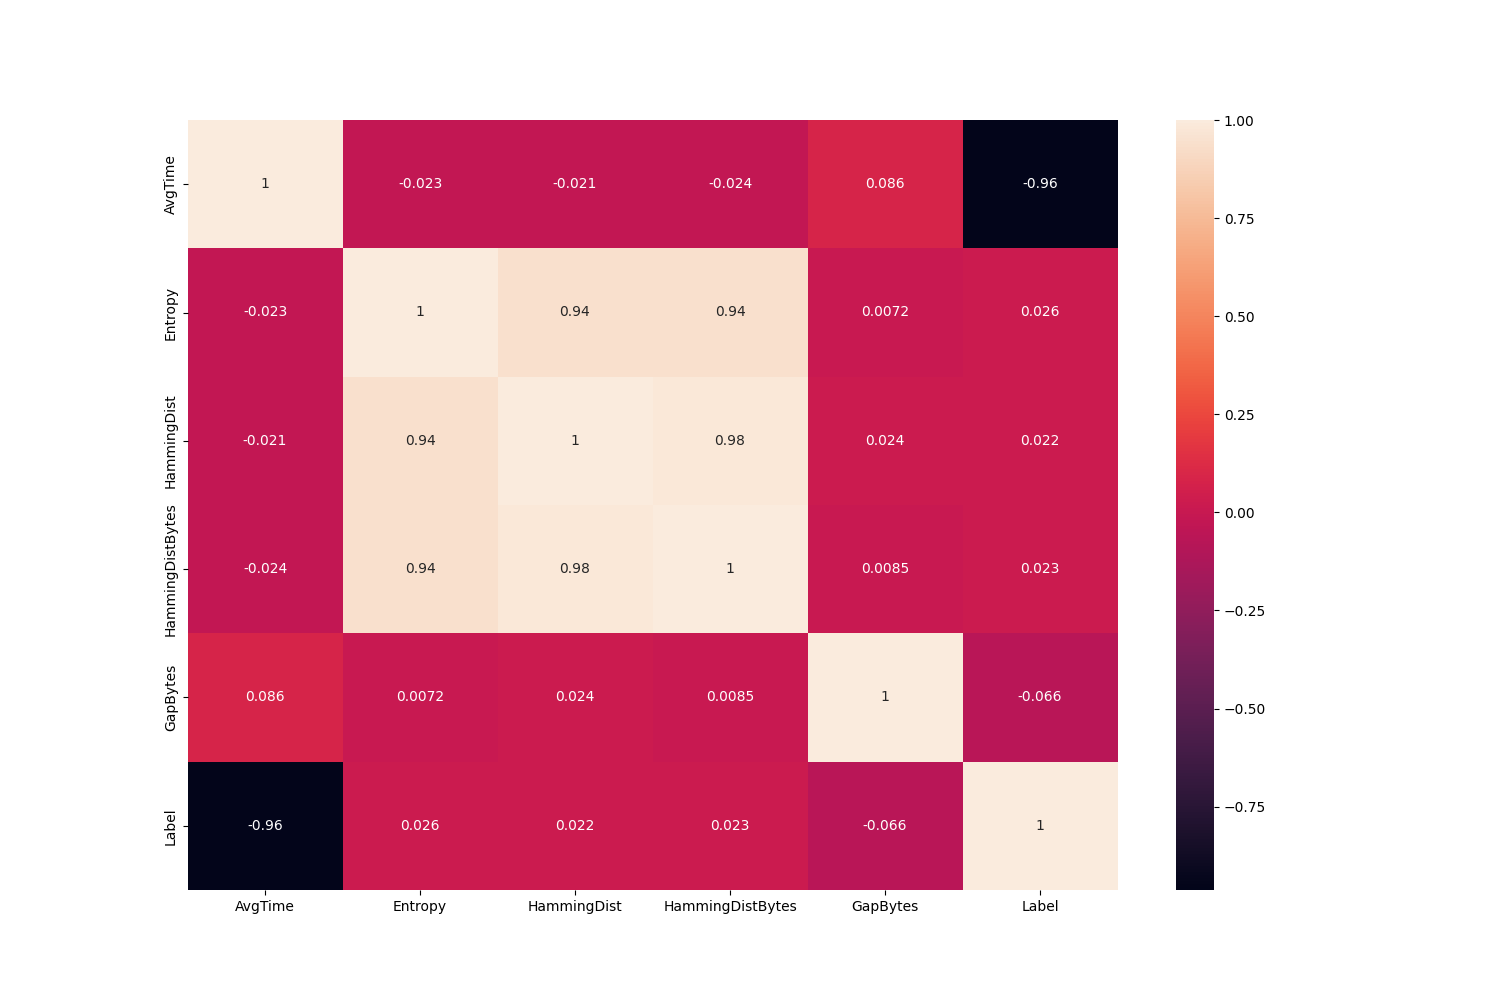
\includegraphics[width = .6\linewidth]{img/parts/app/feature_correlation/OpelAstra/replay.png}
    \caption{Correlation between extracted features obtained from the Automotive Controller Area Network (CAN) Bus Intrusion Dataset v2}
    \label{fig:apdx_fe_tue_opelastra}
\end{figure}

\chapter{Feature extraction}
\label{apdx:sec:feature_extraction}
\begin{figure}
    \centering
    \begin{subfigure}[b]{\linewidth}
        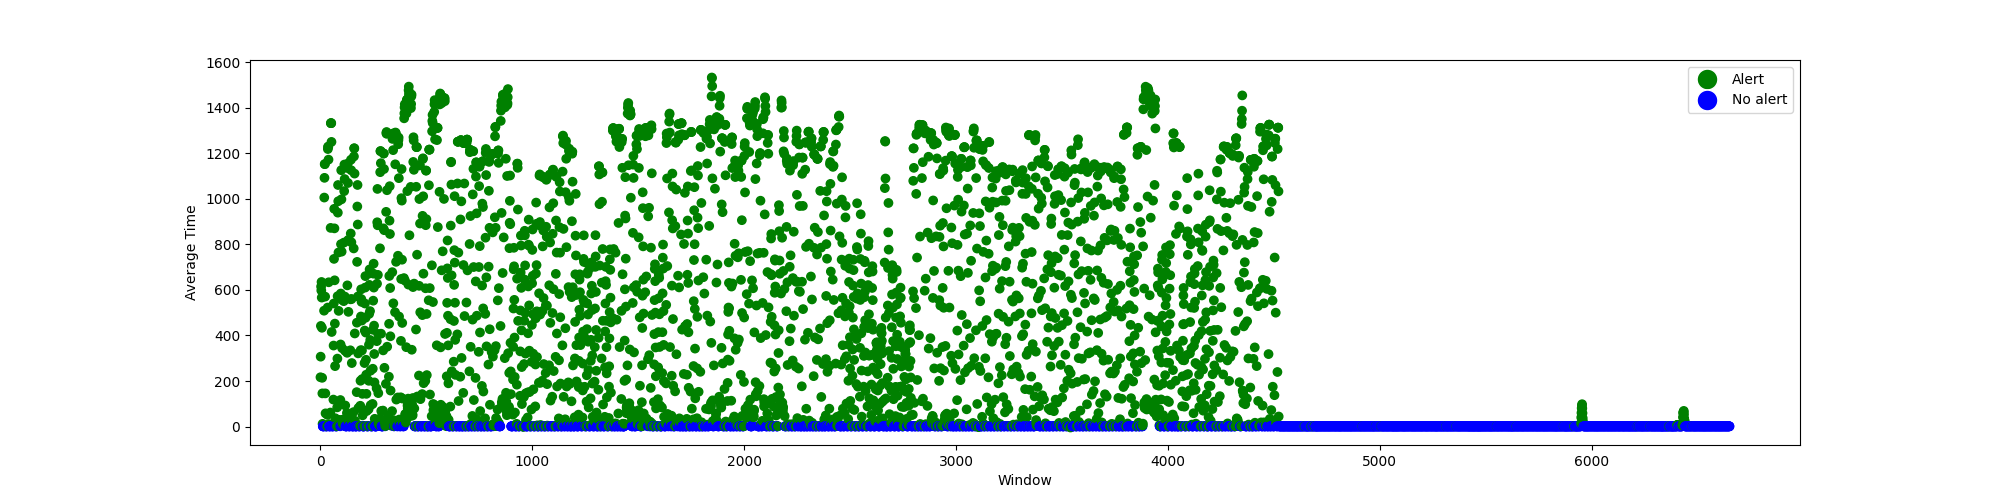
\includegraphics[width = \linewidth]{img/parts/app/tests/car_hacking/DoS/AvgTime.png}
        \caption{Average time between packets}
        \label{subfig:extract_carhacking_dos_avgtime}
    \end{subfigure}
    \begin{subfigure}[b]{\linewidth}
        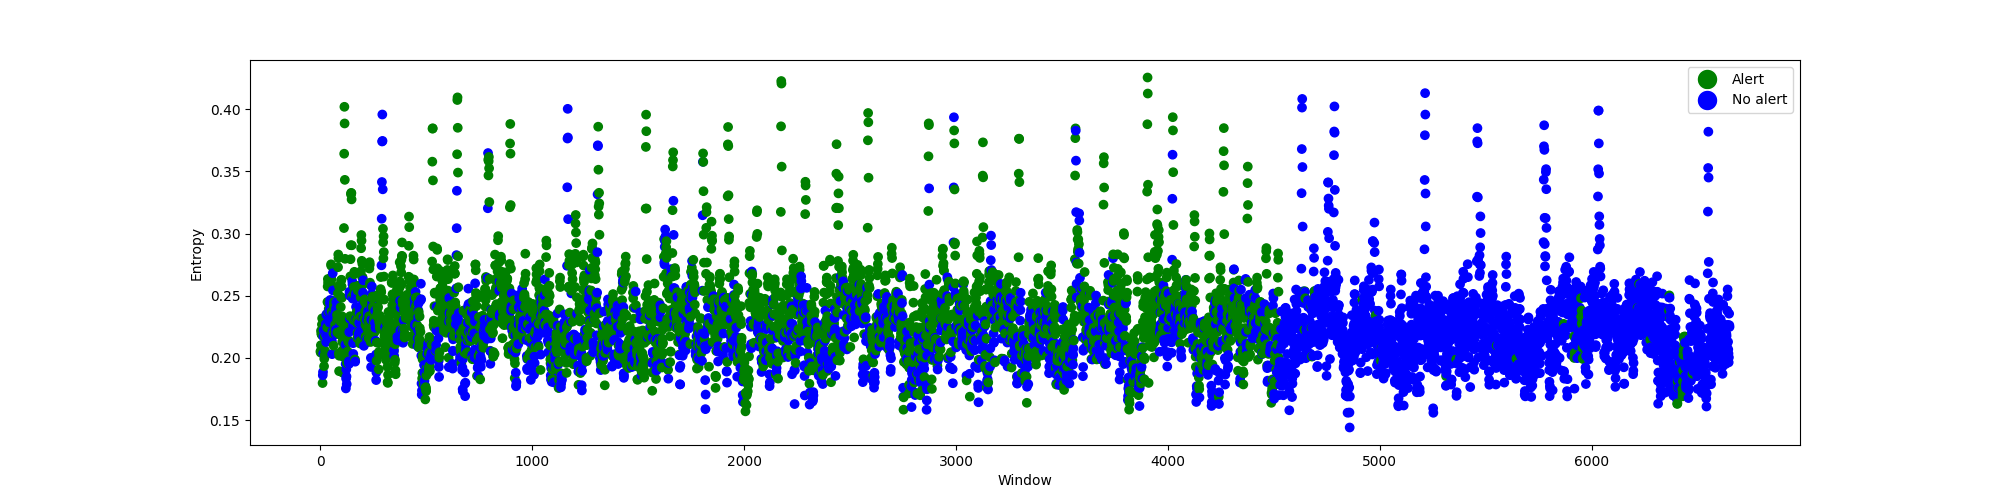
\includegraphics[width = \linewidth]{img/parts/app/tests/car_hacking/DoS/Entropy.png}
        \caption{Average entropy}
        \label{subfig:extract_carhacking_dos_entropy}
    \end{subfigure}
    \begin{subfigure}[b]{\linewidth}
        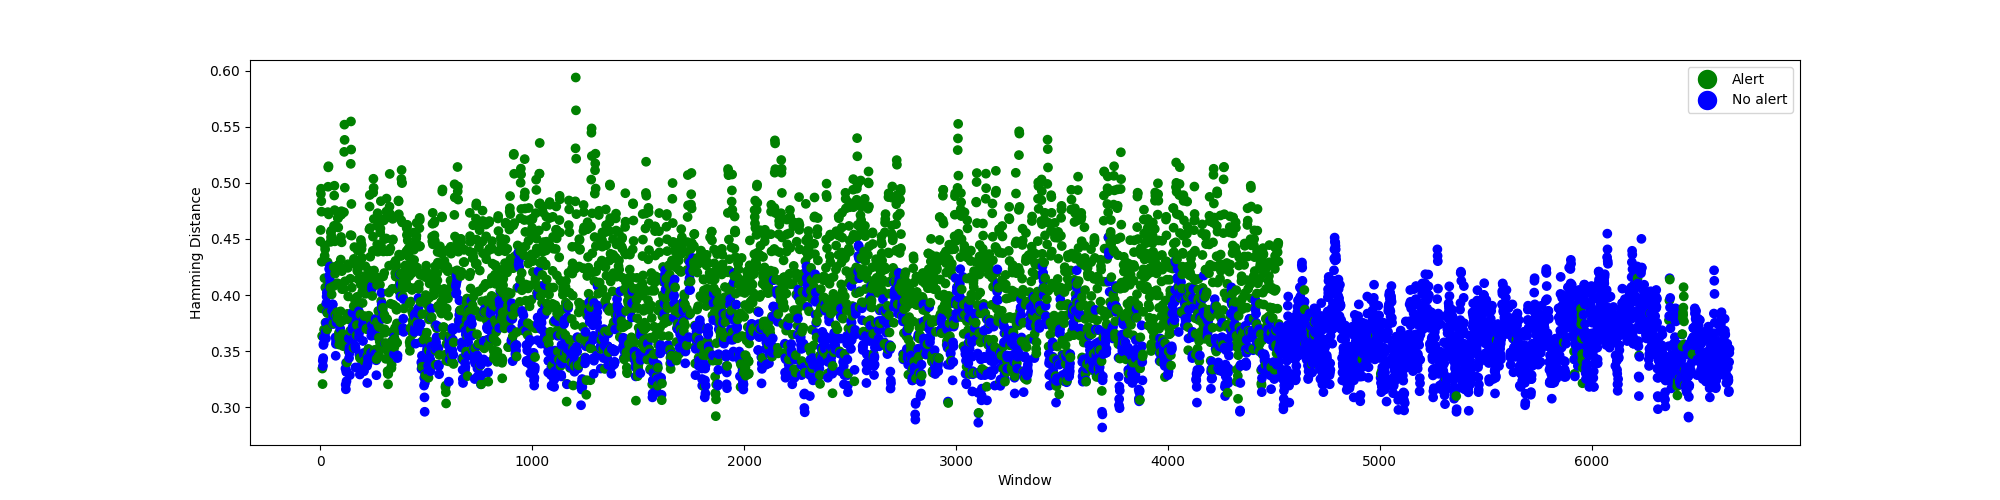
\includegraphics[width = \linewidth]{img/parts/app/tests/car_hacking/DoS/HammingDist.png}
        \caption{Average Hamming distance}
        \label{subfig:extract_carhacking_dos_hammingdist}
    \end{subfigure}
    \caption{Car Hacking - \gls{dos}}
    \label{fig:extract_carhacking_dos}
\end{figure}

\begin{figure}
    \centering
    \begin{subfigure}[b]{\linewidth}
        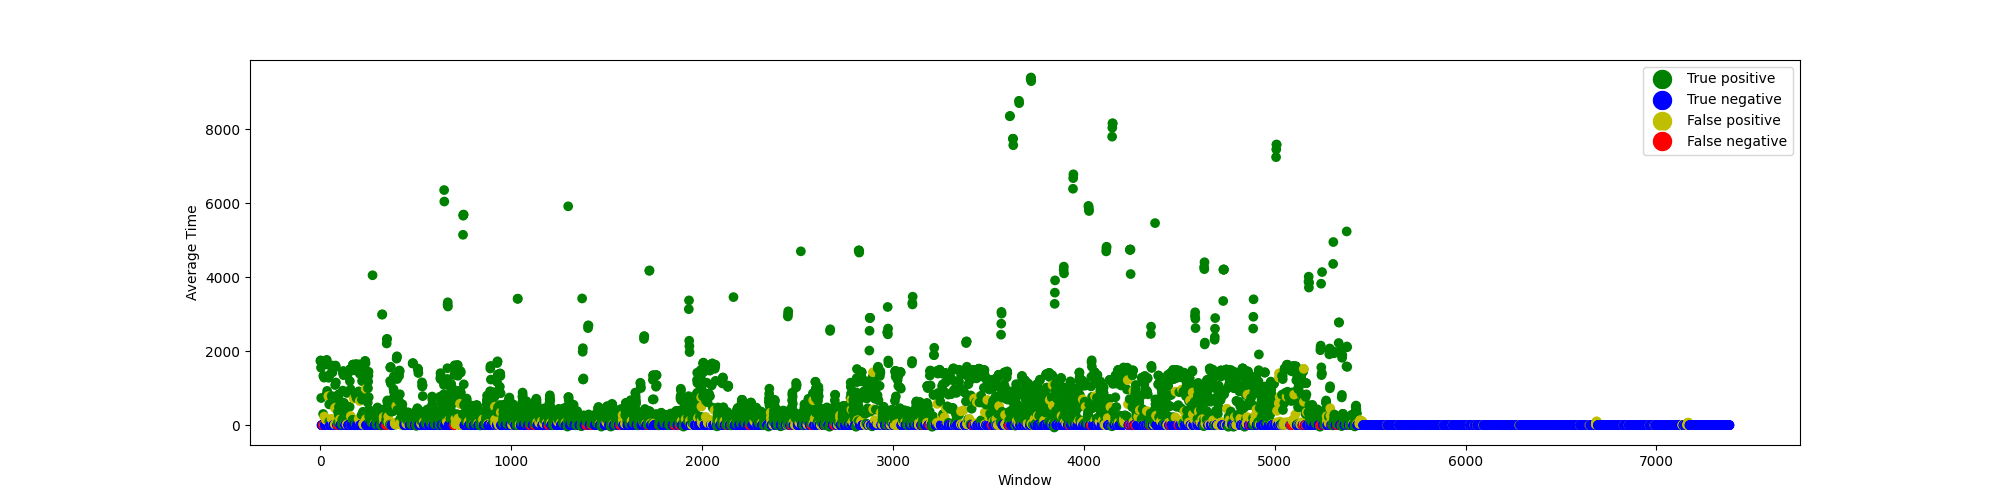
\includegraphics[width = \linewidth]{img/parts/app/tests/car_hacking/fuzzy/AvgTime.png}
        \caption{Average time between packets}
        \label{subfig:extract_carhacking_fuzzy_avgtime}
    \end{subfigure}
    \begin{subfigure}[b]{\linewidth}
        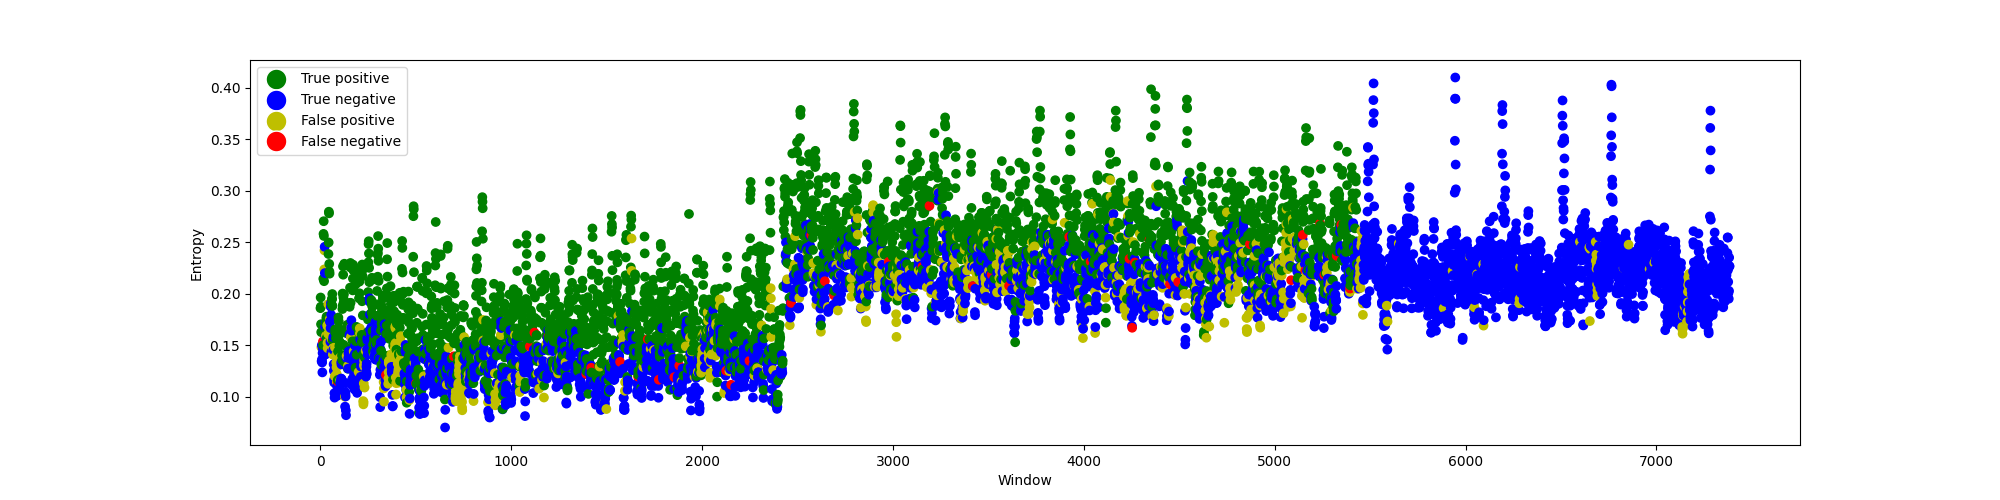
\includegraphics[width = \linewidth]{img/parts/app/tests/car_hacking/fuzzy/Entropy.png}
        \caption{Average entropy}
        \label{subfig:extract_carhacking_fuzzy_entropy}
    \end{subfigure}
    \begin{subfigure}[b]{\linewidth}
        \includegraphics[width = \linewidth]{img/parts/app/tests/car_hacking/fuzzy/HammingDist.png}
        \caption{Average Hamming distance}
        \label{subfig:extract_carhacking_fuzzy_hammingdist}
    \end{subfigure}
    \caption{Car Hacking - Fuzzing}
    \label{fig:extract_carhacking_fuzzy}
\end{figure}

\begin{figure}
    \centering
    \begin{subfigure}[b]{\linewidth}
        \includegraphics[width = \linewidth]{img/parts/app/tests/car_hacking/gear/AvgTime.png}
        \caption{Average time between packets}
        \label{subfig:extract_carhacking_gear_avgtime}
    \end{subfigure}
    \begin{subfigure}[b]{\linewidth}
        \includegraphics[width = \linewidth]{img/parts/app/tests/car_hacking/gear/Entropy.png}
        \caption{Average entropy}
        \label{subfig:extract_carhacking_gear_entropy}
    \end{subfigure}
    \begin{subfigure}[b]{\linewidth}
        \includegraphics[width = \linewidth]{img/parts/app/tests/car_hacking/gear/HammingDist.png}
        \caption{Average Hamming distance}
        \label{subfig:extract_carhacking_gear_hammingdist}
    \end{subfigure}
    \caption{Car Hacking - Gear spoofing}
    \label{fig:extract_carhacking_gear}
\end{figure}

\begin{figure}
    \centering
    \begin{subfigure}[b]{\linewidth}
        \includegraphics[width = \linewidth]{img/parts/app/tests/car_hacking/rpm/AvgTime.png}
        \caption{Average time between packets}
        \label{subfig:extract_carhacking_rpm_avgtime}
    \end{subfigure}
    \begin{subfigure}[b]{\linewidth}
        \includegraphics[width = \linewidth]{img/parts/app/tests/car_hacking/rpm/Entropy.png}
        \caption{Average entropy}
        \label{subfig:extract_carhacking_rpm_entropy}
    \end{subfigure}
    \begin{subfigure}[b]{\linewidth}
        \includegraphics[width = \linewidth]{img/parts/app/tests/car_hacking/rpm/HammingDist.png}
        \caption{Average Hamming distance}
        \label{subfig:extract_carhacking_rpm_hammingdist}
    \end{subfigure}
    \caption{Car Hacking - RPM spoofing}
    \label{fig:extract_carhacking_rpm}
\end{figure}

\begin{figure}
    \centering
    \begin{subfigure}[b]{\linewidth}
        \includegraphics[width = \linewidth]{img/parts/app/tests/ieee/driving/AvgTime.png}
        \caption{Average time between packets}
        \label{subfig:extract_ieee_d_avgtime}
    \end{subfigure}
    \begin{subfigure}[b]{\linewidth}
        \includegraphics[width = \linewidth]{img/parts/app/tests/ieee/driving/Entropy.png}
        \caption{Average entropy}
        \label{subfig:extract_ieee_d_entropy}
    \end{subfigure}
    \begin{subfigure}[b]{\linewidth}
        \includegraphics[width = \linewidth]{img/parts/app/tests/ieee/driving/HammingDist.png}
        \caption{Average Hamming distance}
        \label{subfig:extract_ieee_d_hammingdist}
    \end{subfigure}
    \caption{IEEE Car Hacking: Attack \& Defense Challenge 2020 - Driving Submission}
    \label{fig:extract_ieee_d}
\end{figure}

\begin{figure}
    \centering
    \begin{subfigure}[b]{\linewidth}
        \includegraphics[width = \linewidth]{img/parts/app/tests/ieee/stationary_submission/AvgTime.png}
        \caption{Average time between packets}
        \label{subfig:extract_ieee_s_s_avgtime}
    \end{subfigure}
    \begin{subfigure}[b]{\linewidth}
        \includegraphics[width = \linewidth]{img/parts/app/tests/ieee/stationary_submission/Entropy.png}
        \caption{Average entropy}
        \label{subfig:extract_ieee_s_s_entropy}
    \end{subfigure}
    \begin{subfigure}[b]{\linewidth}
        \includegraphics[width = \linewidth]{img/parts/app/tests/ieee/stationary_submission/HammingDist.png}
        \caption{Average Hamming distance}
        \label{subfig:extract_ieee_s_s_hammingdist}
    \end{subfigure}
    \caption{IEEE Car Hacking: Attack \& Defense Challenge 2020 - Stationary Submission}
    \label{fig:extract_ieee_s_s}
\end{figure}

\begin{figure}
    \centering
    \begin{subfigure}[b]{\linewidth}
        \includegraphics[width = \linewidth]{img/parts/app/tests/ieee/stationary_final/AvgTime.png}
        \caption{Average time between packets}
        \label{subfig:extract_ieee_s_f_avgtime}
    \end{subfigure}
    \begin{subfigure}[b]{\linewidth}
        \includegraphics[width = \linewidth]{img/parts/app/tests/ieee/stationary_final/Entropy.png}
        \caption{Average entropy}
        \label{subfig:extract_ieee_s_f_entropy}
    \end{subfigure}
    \begin{subfigure}[b]{\linewidth}
        \includegraphics[width = \linewidth]{img/parts/app/tests/ieee/stationary_final/HammingDist.png}
        \caption{Average Hamming distance}
        \label{subfig:extract_ieee_s_f_hammingdist}
    \end{subfigure}
    \caption{IEEE Car Hacking: Attack \& Defense Challenge 2020 - Stationary Final}
    \label{fig:extract_ieee_s_f}
\end{figure}

\begin{figure}
    \centering
    \begin{subfigure}[b]{\linewidth}
        \includegraphics[width = \linewidth]{img/parts/app/tests/tue/OpelAstra/fuzzing/AvgTime.png}
        \caption{Average time between packets}
        \label{subfig:extract_tue_opelastra_fuzzing_avgtime}
    \end{subfigure}
    \begin{subfigure}[b]{\linewidth}
        \includegraphics[width = \linewidth]{img/parts/app/tests/tue/OpelAstra/fuzzing/Entropy.png}
        \caption{Average entropy}
        \label{subfig:extract_tue_opelastra_fuzzing_entropy}
    \end{subfigure}
    \begin{subfigure}[b]{\linewidth}
        \includegraphics[width = \linewidth]{img/parts/app/tests/tue/OpelAstra/fuzzing/HammingDist.png}
        \caption{Average Hamming distance}
        \label{subfig:extract_tue_opelastra_fuzzing_hammingdist}
    \end{subfigure}
    \caption{Automotive Controller Area Network (CAN) Bus Intrusion Dataset v2 - Opel Astra - Fuzzing attack}
    \label{fig:extract_tue_opelastra_fuzzing}
\end{figure}

\begin{figure}
    \centering
    \begin{subfigure}[b]{\linewidth}
        \includegraphics[width = \linewidth]{img/parts/app/tests/tue/OpelAstra/deletion/AvgTime.png}
        \caption{Average time between packets}
        \label{subfig:extract_tue_opelastra_deletion_avgtime}
    \end{subfigure}
    \begin{subfigure}[b]{\linewidth}
        \includegraphics[width = \linewidth]{img/parts/app/tests/tue/OpelAstra/deletion/Entropy.png}
        \caption{Average entropy}
        \label{subfig:extract_tue_opelastra_deletion_entropy}
    \end{subfigure}
    \begin{subfigure}[b]{\linewidth}
        \includegraphics[width = \linewidth]{img/parts/app/tests/tue/OpelAstra/deletion/HammingDist.png}
        \caption{Average Hamming distance}
        \label{subfig:extract_tue_opelastra_deletion_hammingdist}
    \end{subfigure}
    \caption{Automotive Controller Area Network (CAN) Bus Intrusion Dataset v2 - Opel Astra - Message deletion attack}
    \label{fig:extract_tue_opelastra_deletion}
\end{figure}

\begin{figure}
    \centering
    \begin{subfigure}[b]{\linewidth}
        \includegraphics[width = \linewidth]{img/parts/app/tests/tue/OpelAstra/replay/AvgTime.png}
        \caption{Average time between packets}
        \label{subfig:extract_tue_opelastra_replay_avgtime}
    \end{subfigure}
    \begin{subfigure}[b]{\linewidth}
        \includegraphics[width = \linewidth]{img/parts/app/tests/tue/OpelAstra/replay/Entropy.png}
        \caption{Average entropy}
        \label{subfig:extract_tue_opelastra_replay_entropy}
    \end{subfigure}
    \begin{subfigure}[b]{\linewidth}
        \includegraphics[width = \linewidth]{img/parts/app/tests/tue/OpelAstra/replay/HammingDist.png}
        \caption{Average Hamming distance}
        \label{subfig:extract_tue_opelastra_replay_hammingdist}
    \end{subfigure}
    \caption{Automotive Controller Area Network (CAN) Bus Intrusion Dataset v2 - Opel Astra - Replay attack}
    \label{fig:extract_tue_opelastra_replay}
\end{figure}

\begin{figure}
    \centering
    \begin{subfigure}[b]{\linewidth}
        \includegraphics[width = \linewidth]{img/parts/app/tests/tue/RenaultClio/fuzzing/AvgTime.png}
        \caption{Average time between packets}
        \label{subfig:extract_tue_renaultclio_fuzzing_avgtime}
    \end{subfigure}
    \begin{subfigure}[b]{\linewidth}
        \includegraphics[width = \linewidth]{img/parts/app/tests/tue/RenaultClio/fuzzing/Entropy.png}
        \caption{Average entropy}
        \label{subfig:extract_tue_renaultclio_fuzzing_entropy}
    \end{subfigure}
    \begin{subfigure}[b]{\linewidth}
        \includegraphics[width = \linewidth]{img/parts/app/tests/tue/RenaultClio/fuzzing/HammingDist.png}
        \caption{Average Hamming distance}
        \label{subfig:extract_tue_renaultclio_fuzzing_hammingdist}
    \end{subfigure}
    \caption{Automotive Controller Area Network (CAN) Bus Intrusion Dataset v2 - Renault Clio - Fuzzing attack}
    \label{fig:extract_tue_renaultclio_fuzzing}
\end{figure}

\begin{figure}
    \centering
    \begin{subfigure}[b]{\linewidth}
        \includegraphics[width = \linewidth]{img/parts/app/tests/tue/RenaultClio/deletion/AvgTime.png}
        \caption{Average time between packets}
        \label{subfig:extract_tue_renaultclio_deletion_avgtime}
    \end{subfigure}
    \begin{subfigure}[b]{\linewidth}
        \includegraphics[width = \linewidth]{img/parts/app/tests/tue/RenaultClio/deletion/Entropy.png}
        \caption{Average entropy}
        \label{subfig:extract_tue_renaultclio_deletion_entropy}
    \end{subfigure}
    \begin{subfigure}[b]{\linewidth}
        \includegraphics[width = \linewidth]{img/parts/app/tests/tue/RenaultClio/deletion/HammingDist.png}
        \caption{Average Hamming distance}
        \label{subfig:extract_tue_renaultclio_deletion_hammingdist}
    \end{subfigure}
    \caption{Automotive Controller Area Network (CAN) Bus Intrusion Dataset v2 - Renault Clio - Message deletion attack}
    \label{fig:extract_tue_renaultclio_deletion}
\end{figure}

\begin{figure}
    \centering
    \begin{subfigure}[b]{\linewidth}
        \includegraphics[width = \linewidth]{img/parts/app/tests/tue/RenaultClio/replay/AvgTime.png}
        \caption{Average time between packets}
        \label{subfig:extract_tue_renaultclio_replay_avgtime}
    \end{subfigure}
    \begin{subfigure}[b]{\linewidth}
        \includegraphics[width = \linewidth]{img/parts/app/tests/tue/RenaultClio/replay/Entropy.png}
        \caption{Average entropy}
        \label{subfig:extract_tue_renaultclio_replay_entropy}
    \end{subfigure}
    \begin{subfigure}[b]{\linewidth}
        \includegraphics[width = \linewidth]{img/parts/app/tests/tue/RenaultClio/replay/HammingDist.png}
        \caption{Average Hamming distance}
        \label{subfig:extract_tue_renaultclio_replay_hammingdist}
    \end{subfigure}
    \caption{Automotive Controller Area Network (CAN) Bus Intrusion Dataset v2 - Renault Clio - Replay attack}
    \label{fig:extract_tue_renaultclio_replay}
\end{figure}

\begin{figure}
    \centering
    \begin{subfigure}[b]{\linewidth}
        \includegraphics[width = \linewidth]{img/parts/app/tests/crysys/add_incr/AvgTime.png}
        \caption{Average time between packets}
        \label{subfig:extract_crysys_addincr_avgtime}
    \end{subfigure}
    \begin{subfigure}[b]{\linewidth}
        \includegraphics[width = \linewidth]{img/parts/app/tests/crysys/add_incr/Entropy.png}
        \caption{Average entropy}
        \label{subfig:extract_crysys_addincr_entropy}
    \end{subfigure}
    \begin{subfigure}[b]{\linewidth}
        \includegraphics[width = \linewidth]{img/parts/app/tests/crysys/add_incr/HammingDist.png}
        \caption{Average Hamming distance}
        \label{subfig:extract_crysys_addincr_hammingdist}
    \end{subfigure}
    \caption{Modified CrySyS Lab - Adding an increasing value}
    \label{fig:extract_crysys_addincr}
\end{figure}

\begin{figure}
    \centering
    \begin{subfigure}[b]{\linewidth}
        \includegraphics[width = \linewidth]{img/parts/app/tests/crysys/const/AvgTime.png}
        \caption{Average time between packets}
        \label{subfig:extract_crysys_const_avgtime}
    \end{subfigure}
    \begin{subfigure}[b]{\linewidth}
        \includegraphics[width = \linewidth]{img/parts/app/tests/crysys/const/Entropy.png}
        \caption{Average entropy}
        \label{subfig:extract_crysys_const_entropy}
    \end{subfigure}
    \begin{subfigure}[b]{\linewidth}
        \includegraphics[width = \linewidth]{img/parts/app/tests/crysys/const/HammingDist.png}
        \caption{Average Hamming distance}
        \label{subfig:extract_crysys_const_hammingdist}
    \end{subfigure}
    \caption{Modified CrySyS Lab - Constant value}
    \label{fig:extract_crysys_const}
\end{figure}

\begin{figure}
    \centering
    \begin{subfigure}[b]{\linewidth}
        \includegraphics[width = \linewidth]{img/parts/app/tests/crysys/decr/AvgTime.png}
        \caption{Average time between packets}
        \label{subfig:extract_crysys_decr_avgtime}
    \end{subfigure}
    \begin{subfigure}[b]{\linewidth}
        \includegraphics[width = \linewidth]{img/parts/app/tests/crysys/decr/Entropy.png}
        \caption{Average entropy}
        \label{subfig:extract_crysys_decr_entropy}
    \end{subfigure}
    \begin{subfigure}[b]{\linewidth}
        \includegraphics[width = \linewidth]{img/parts/app/tests/crysys/decr/HammingDist.png}
        \caption{Average Hamming distance}
        \label{subfig:extract_crysys_decr_hammingdist}
    \end{subfigure}
    \caption{Modified CrySyS Lab - Decreasing value}
    \label{fig:extract_crysys_decr}
\end{figure}

\begin{figure}
    \centering
    \begin{subfigure}[b]{\linewidth}
        \includegraphics[width = \linewidth]{img/parts/app/tests/crysys/delta/AvgTime.png}
        \caption{Average time between packets}
        \label{subfig:extract_crysys_delta_avgtime}
    \end{subfigure}
    \begin{subfigure}[b]{\linewidth}
        \includegraphics[width = \linewidth]{img/parts/app/tests/crysys/delta/Entropy.png}
        \caption{Average entropy}
        \label{subfig:extract_crysys_delta_entropy}
    \end{subfigure}
    \begin{subfigure}[b]{\linewidth}
        \includegraphics[width = \linewidth]{img/parts/app/tests/crysys/delta/HammingDist.png}
        \caption{Average Hamming distance}
        \label{subfig:extract_crysys_delta_hammingdist}
    \end{subfigure}
    \caption{Modified CrySyS Lab - Delta of 1000}
    \label{fig:extract_crysys_delta}
\end{figure}

\begin{figure}
    \centering
    \begin{subfigure}[b]{\linewidth}
        \includegraphics[width = \linewidth]{img/parts/app/tests/crysys/rand/AvgTime.png}
        \caption{Average time between packets}
        \label{subfig:extract_crysys_rand_avgtime}
    \end{subfigure}
    \begin{subfigure}[b]{\linewidth}
        \includegraphics[width = \linewidth]{img/parts/app/tests/crysys/rand/Entropy.png}
        \caption{Average entropy}
        \label{subfig:extract_crysys_rand_entropy}
    \end{subfigure}
    \begin{subfigure}[b]{\linewidth}
        \includegraphics[width = \linewidth]{img/parts/app/tests/crysys/rand/HammingDist.png}
        \caption{Average Hamming distance}
        \label{subfig:extract_crysys_rand_hammingdist}
    \end{subfigure}
    \caption{Modified CrySyS Lab - Random value}
    \label{fig:extract_crysys_rand}
\end{figure}

\chapter{Code documentation}
\label{apdx:sec:code_documentation}
\chapter{Code documentation}
\label{apdx:sec:code_documentation}

This chapter presents the source code documentation. It aims to provide a high-level understanding of the application's funcionality as well as the API it provides.

\begin{figure}
    \centering
    \includegraphics[width = \linewidth]{img/parts/docs/crate.png}
    \caption{Crate AIHDS}
    \label{fig:doc_crate}
\end{figure}

\begin{figure}
    \centering
    \begin{subfigure}[b]{\linewidth}
        \includegraphics[width = \linewidth]{img/parts/docs/dataset/dataset.png}
        \caption{Module}
        \label{subfig:doc_dataset}
    \end{subfigure}
    \begin{subfigure}[b]{\linewidth}
        \includegraphics[width = \linewidth]{img/parts/docs/dataset/dataset_normalize.png}
        \caption{\emph{normalize} function}
        \label{subfig:doc_dataset_normalize}
    \end{subfigure}
    \begin{subfigure}[b]{\linewidth}
        \includegraphics[width = \linewidth]{img/parts/docs/dataset/dataset_packetsfromcsv.png}
        \caption{\emph{packets\_from\_csv} function}
        \label{subfig:doc_dataset_packetsfromcsv}
    \end{subfigure}
    \caption{\emph{Dataset} module}
    \label{fig:doc_dataset}
\end{figure}
\begin{figure}
    \ContinuedFloat
    \begin{subfigure}[b]{\linewidth}
        \includegraphics[width = \linewidth]{img/parts/docs/dataset/dataset_writefeatures.png}\
        \caption{\emph{write\_features} function}
        \label{subfig:doc_dataset_writefeatures}
    \end{subfigure}
    \begin{subfigure}[b]{\linewidth}
        \includegraphics[width = \linewidth]{img/parts/docs/dataset/dataset\_writefeaturesunsupervised.png}
        \caption{\emph{write\_features\_unsupervised} function}
        \label{subfig:doc_dataset_writefeaturesunsupervised}
    \end{subfigure}
    \caption{\emph{Dataset} module (cont.)}
    \label{fig:doc_dataset}
\end{figure}

\begin{figure}
    \centering
    \begin{subfigure}[b]{\linewidth}
        \includegraphics[width = \linewidth]{img/parts/docs/ids/ids.png}
        \caption{Module}
        \label{subfig:doc_ids}
    \end{subfigure}
    \begin{subfigure}[b]{\linewidth}
        \includegraphics[width = \linewidth]{img/parts/docs/ids/ids_struct.png}
        \caption{Struct}
        \label{subfig:doc_ids_struct}
    \end{subfigure}
    \caption{\emph{IDS} module}
    \label{fig:doc_ids}
\end{figure}
\begin{figure}
    \ContinuedFloat
    \begin{subfigure}[b]{\linewidth}
        \includegraphics[width = \linewidth]{img/parts/docs/ids/ids_struct_new.png}
        \caption{IDS' \emph{new} function}
        \label{subfig:doc_ids_stuct_new}
    \end{subfigure}
    \begin{subfigure}[b]{\linewidth}
        \includegraphics[width = \linewidth]{img/parts/docs/ids/ids_struct_load.png}
        \caption{\emph{load} function}
        \label{subfig:doc_ids_stuct_load}
    \end{subfigure}
    \begin{subfigure}[b]{\linewidth}
        \includegraphics[width = \linewidth]{img/parts/docs/ids/ids_struct_getmonitor.png}
        \caption{\emph{get\_monitor} function}
        \label{subfig:doc_ids_stuct_getmonitor}
    \end{subfigure}
    \caption{\emph{IDS} module (cont.)}
    \label{fig:doc_ids}
\end{figure}
\begin{figure}
    \ContinuedFloat
    \begin{subfigure}[b]{\linewidth}
        \includegraphics[width = \linewidth]{img/parts/docs/ids/ids_struct_train.png}
        \caption{\emph{train} function}
        \label{subfig:doc_ids_stuct_train}
    \end{subfigure}
    \begin{subfigure}[b]{\linewidth}
        \includegraphics[width = \linewidth]{img/parts/docs/ids/ids_struct_test.png}
        \caption{\emph{test} function}
        \label{subfig:doc_ids_stuct_test}
    \end{subfigure}
    \caption{\emph{IDS} module (cont.)}
    \label{fig:doc_ids}
\end{figure}
\begin{figure}
    \ContinuedFloat
    \begin{subfigure}[b]{\linewidth}
        \includegraphics[width = \linewidth]{img/parts/docs/ids/ids_struct_featureset.png}
        \caption{\emph{feature\_set} function}
        \label{subfig:doc_ids_stuct_featureset}
    \end{subfigure}
    \begin{subfigure}[b]{\linewidth}
        \includegraphics[width = \linewidth]{img/parts/docs/ids/ids_struct_push.png}
        \caption{\emph{push} function}
        \label{subfig:doc_ids_stuct_push}
    \end{subfigure}
    \begin{subfigure}[b]{\linewidth}
        \includegraphics[width = \linewidth]{img/parts/docs/ids/ids_struct_predict.png}
        \caption{\emph{predict} function}
        \label{subfig:doc_ids_stuct_predict}
    \end{subfigure}
    \caption{\emph{IDS} module (cont.)}
    \label{fig:doc_ids}
\end{figure}
\begin{figure}
    \ContinuedFloat
    \begin{subfigure}[b]{\linewidth}
        \includegraphics[width = \linewidth]{img/parts/docs/ids/ids_struct_extractfeatures.png}
        \caption{\emph{extract\_features} function}
        \label{subfig:doc_ids_stuct_extractfeatures}
    \end{subfigure}
    \begin{subfigure}[b]{\linewidth}
        \includegraphics[width = \linewidth]{img/parts/docs/ids/packet_struct.png}
        \caption{\emph{Packet} struct}
        \label{subfig:doc_packet_struct}
    \end{subfigure}
    \begin{subfigure}[b]{\linewidth}
        \includegraphics[width = \linewidth]{img/parts/docs/ids/packet_struct_new.png}
        \caption{Packet's \emph{new} function}
        \label{subfig:doc_packet_struct_new}
    \end{subfigure}
    \caption{\emph{IDS} module (cont.)}
    \label{fig:doc_ids}
\end{figure}
\begin{figure}
    \ContinuedFloat
    \begin{subfigure}[b]{\linewidth}
        \includegraphics[width = \linewidth]{img/parts/docs/ids/ids_type_features.png}
        \caption{\emph{Features} type}
        \label{subfig:doc_ids_type_features}
    \end{subfigure}
    \begin{subfigure}[b]{\linewidth}
        \includegraphics[width = \linewidth]{img/parts/docs/ids/ids_type_prediction.png}
        \caption{\emph{Prediction} type}
        \label{subfig:doc_ids_type_prediction}
    \end{subfigure}
    \caption{\emph{IDS} module (cont.)}
    \label{fig:doc_ids}
\end{figure}

\begin{figure}
    \centering
    \begin{subfigure}[b]{\linewidth}
        \includegraphics[width = \linewidth]{img/parts/docs/server/server.png}
        \caption{Module}
        \label{subfig:doc_server}
    \end{subfigure}
    \begin{subfigure}[b]{\linewidth}
        \includegraphics[width = \linewidth]{img/parts/docs/server/server_opensocket.png}
        \caption{\emph{open\_socket} function}
        \label{subfig:doc_server_opensocket}
    \end{subfigure}
    \begin{subfigure}[b]{\linewidth}
        \includegraphics[width = \linewidth]{img/parts/docs/server/server_post.png}
        \caption{\emph{post} function}
        \label{subfig:doc_server_post}
    \end{subfigure}
    \caption{\emph{Server} module}
    \label{fig:doc_server}
\end{figure}

\begin{backcover}
\thispagestyle{empty} \pagecolor{white} \textcolor{black} {\fontfamily{phv}\fontseries{mc}\selectfont ~\vfill
\noindent
% NB: place here information about funding, FCT project, etc in which the work is framed. Leave empty otherwise.
%
\vfill ~}
\end{backcover}

\end{document}